% paper size is in preamble.sty
\documentclass[10pt,openany,table,x11names]{book}

% Continuous footnote numbering across all chapters (don't reset at \chapter)
\makeatletter
\@removefromreset{footnote}{chapter}
\makeatother

\newenvironment{smallquote}
  {\begin{quote}\small}
  {\end{quote}}

% meta data
\newcommand{\authorname}{Kirill Eskrov}
\newcommand{\booktitle}{The Gospel of Afranius}
\newcommand{\subtitle}{A Detective Investigation into Sacred History}
\newcommand{\publisher}{Me}
\newcommand{\editionyear}{1997}
\newcommand{\isbn}{}

% Load options (and fontspec) before title so we can use \fontspec for title font
\usepackage{misc/options}

% Title font: use monospace if available (cursor-style); otherwise document default
\IfFontExistsTF{texgyrecursor-regular.otf}{%
  {\fontspec{texgyrecursor-regular.otf}\title{\booktitle}}%
}{%
  \title{\booktitle}%
}
\author{\authorname}
\begin{document}

% Front matter
\frontmatter
% Página de título (contra-capa)
\begin{titlepage}
    \centering
    \newgeometry{top=1in,bottom=1in,right=0in,left=0in}
    \thispagestyle{empty}

    % Title
    % Mess with the font size here
    \vspace{6pt}
    {\Huge\booktitle}

    % Subtitle
    {
        \vspace{25pt}
        \begin{minipage}{10cm}{
            \Large\emph{\subtitle}
        }
        \end{minipage}
	
	% \vspace{\stretch{1.25}}
    }
    

    % Editora
    \vspace{\stretch{6}}
    {
        % {\scshape\large \authorname\par}
        % \Huge\scshape\large\publisher\par
    }
\end{titlepage}

% Página de copyright
\vfill

\begin{center}
    Original Russian edition {\oldenglishfont ©} \editionyear{} Kirill Eskov \\ (afranius999@gmail.com)
\end{center}

\begin{center}
    English translation {\oldenglishfont ©} Zachary Baumgartner \\ (zachary.m.baumgartner@gmail.com)
\end{center}

\begin{center}
    Illustrations {\oldenglishfont ©} 2018 Yevgeny Melnikov \\ (barbus18@ya.ru)
\end{center}

\vfill

\begin{center}
    \emph{Translator's note:}
\end{center}

This translation was produced in close collaboration with the original
author, without whose invaluable input (and moral support) this project would never have gotten off the ground. To call me appreciative would be a massive understatement.

At times, I have found it necessary to add explanatory notes alongside
Eskov's original footnotes. To prevent confusion, each set is marked with our respective initials; citations, however, remain unmarked.

Happy reading!
\cleardoublepage
\thispagestyle{empty}
\begingroup
  \makeatletter
  \let\addcontentsline\@gobblethree % don't write "Contents" into the .toc
  \makeatother
  \renewcommand{\contentsname}{{\Huge Table of Contents}} % optional
  \tableofcontents
\endgroup
\cleardoublepage
% \input{frontmatter/preface}
% \input{frontmatter/timeline}

% Main matter
\mainmatter
\pagestyle{fancy}

% contents
% No \chapter here (the preface opens straight into the epigraph), so set the running
% head and TOC entry by hand. Without this, \leftmark keeps the stale "Table of Contents"
% mark and it leaks onto the preface pages.
\addcontentsline{toc}{chapter}{Preface}
\markboth{Preface}{}

% TODO: float me right
\vspace*{\fill}
    \noindent
    {\itshape\footnotesize 
       ``Take care what you're doing, Afranius. After all, they're temple seals!'' \\
       ``The procurator need not trouble himself about this question,'' replied Afranius, closing the packet. \\ ``You mean you have all their seals?'' asked Pilate, laughing. \\ 
       ``How could it be otherwise,'' replied Afranius dryly, with no trace of laughter. 
    }
    \vspace{2em}

    \noindent\hfill\hspace*{-1.5em}
    {{\large --- Mikhail Bulgakov} \\}
    \vspace{1em}
    \noindent\hfill\hspace*{-1.5em}
    {\textit{The Master and Margarita}\footnote{trans. Diana Burgin \& Katherine Tiernan O'Connor, pp. 275-276}}
\vspace*{\fill}

Borges once remarked that ``the generations of men, throughout recorded time, have always told and retold two stories---that of a lost ship which searches the Mediterranean seas for a dearly loved island, and that of a god who is crucified on Golgotha.''\footnote{
``The Gospel According to Mark'' from \emph{Dr. Brodie's Report}, trans. Norman Thomas di Giovanni, p. 9.}With regard to the latter, he was perhaps not entirely correct. The artistic and philosophical reinterpretation of the events surrounding the execution of Jesus Christ only became an established literary tradition in the 19\textsuperscript{th} century, when the Church lost a significant portion of its function of ideological supervision. Within a narrative, this theme typically takes the form of a subplot or a ``novel within a novel'' (as in the works of Bulgakov and Aitmatov); more rarely, it may take the form of a standalone work (such as those of France and Andreyev).\footnote{The works Yeskov is referencing are \emph{The Master and Margarita} by Mikhail Bulgakov, \emph{The Place of the
Skull} by Chingiz Aitmatov, ``The Procurator of Judea'' by Anatole France, and ``On the Day of the
Crucifixion'' by Leonid Andreyev. (Z.B.)} The texts that have been created within this tradition vary quite widely, both in their artistic level (from Bulgakov's immortal \emph{Master} to Ilya Varshavsky's comic sci-fi story ``Hysteresis Loop'') and in the degree to which they conform to Holy Scripture and historical reality (from the pinpoint precision of Yury Dombrovsky to the deliberate inaccuracy of the Strugatsky brothers).\footnote{These works are, respectively, \emph{The Faculty of Useless Knowledge and Burdened with Evil.} (Z.B.)} With regard to the latter aspect, it is worth comparing two renowned cinematic masterpieces: \emph{The Gospel According to St. Matthew} and \emph{The Last Temptation of Christ}. It goes without saying that all these authors' versions differ quite radically, to the point where the Gospel figures depicted in them are merely ``homonyms'' of each other---compare France's Pilate with Bulgakov's, Andreyev's Judas with Dombrovsky's, or Pasolini's Jesus with Scorcese's.

Nevertheless, there is still one fundamental constraint that all works produced within this tradition are subject to: supernatural forces may not directly interfere with the course of events other than to send ``a strange cloud drifting into Yershalaim.''\footnote{\emph{The Master and Margarita}, p. 255. ``Yershalaim'' is the Russian transliteration of the Hebrew word ``Yerushalayim,'' meaning ``Jerusalem.'' (Z.B.)} This is precisely why an event so crucial to the Christian worldview as the Bodily Resurrection is always omitted from these narratives---despite the fact that many of the authors who have turned to this theme were undoubtedly people of faith. And since I belong to a generation whose perceptions were shaped immeasurably more by Bulgakov's Yeshua\footnote{Similarly to his use of the word ``Yershalaim'' (see note 6), Bulgakov refers to Jesus in \emph{The Master and Margarita} by his Aramaic name, Yeshua Ha-Notsri. (Z.B.)} than by his official prototype, the problem of the Resurrection was one that did not interest me in the slightest up until very recently.
\newpage
\begin{center}
    \Huge McDowell's Argument
\end{center}

Not long ago, however, I came across a book by famed contemporary evangelist Josh McDowell,\footnote{\emph{The Resurrection Factor}. San Bernardino, CA: Here's Life Publishers, 1981} in which he sets himself a most extraordinary task: to prove the fact of Christ's Bodily Resurrection from a \emph{purely rational perspective.} McDowell's system of reasoning is as follows. Treating the Gospel as a historical document and drawing on a number of other (religiously neutral) sources, he meticulously sorts through all conceivable possibilities that might provide a materialist explanation for the extraordinary events following the execution of Jesus Christ (in particular, the disappearance of his body from a sealed tomb that was guarded by Roman soldiers). He classifies these hypotheses in the following manner:

\begin{enumerate}
    \item[I.] \emph{Christ's tomb was not actually empty.}
    \begin{enumerate}
        \item[1.] The actual location of Christ's burial was completely unknown; his body was most likely tossed into a ditch alongside those of the other executed criminals (Guignebert's hypothesis).\footnote{I.e. French Historian Charles Guignebert. (Z.B.)}
        \item[2.] Confusion with the tombs: the women who first discovered the ``Resurrection'' actually went to another person's unoccupied tomb by mistake (Lake's hypothesis).\footnote{I.e. Harvard professor Kirsopp Lake. (Z.B.)}
        \item[3.] All stories of the Resurrection are legends that sprang up many years after Christ's execution, and have no basis in reality whatsoever.
        \item[4.] The story of the Resurrection is merely an allegory; what it describes is actually a purely spiritual resurrection.
        \item[5.] All of Christ's appearances were the result of individual and collective hallucinations.
    \end{enumerate}
    \item[II.] \emph{Christ's tomb actually was empty, but was made empty by natural
    means.}
    \begin{enumerate}
        \item[1.] His body was stolen by his disciples.
        \item[2.] His body was relocated and hidden by the authorities, with the goal of preventing any possible fraud on the part of those who were awaiting his resurrection.
        \item[3.] Christ did not die on the cross; he was taken down from it in a state of shock, then later regained consciousness and recovered. 
        \item[4.] Hugh Schonfield's Passover Plot hypothesis: Jesus, believing that he was chosen by God, set out to create the appearance of fulfilling the prophecies concerning the Messiah. To this end, he organized his own crucifixion with the help of Joseph of Arimathea; to imitate death on the cross, he drank a narcotic substance instead of vinegar. According to the plan, he would then be brought into the tomb, from which he would emerge sometime later as the ``resurrected'' Christ. The plot failed when a soldier struck Christ with his spear and killed him for real. However, Mary and the disciples then went on to mistake another young man for Christ; Joseph, despite knowing the truth, never thought to inform them of their error. 
    \end{enumerate}
\end{enumerate}

After refuting all these hypotheses to varying degrees of persuasiveness, McDowell considers the range of logical possibilities to be exhausted and comes to a conclusion: it is impossible to explain the disappearance of Christ's body, as well as his subsequent appearances, from a materialist perspective. \emph{Ergo}, we are presented with a case of the direct intervention of God in earthly affairs.

It should be noted that a completely identical system of proof for Christ's resurrection had already been laid out in 1906 in Boris Gladkov's \emph{Universally Accessible Interpretation of the Gospel}, a book ``intended for intelligent readers, especially nonbelievers, doubters, and vacillators.''\footnote{\emph{Universally Accessible Interpretation of the Gospel,} annotation.} Likewise, he sequentially refutes ``three possible objections to the reality of Christ's resurrection'':

\begin{smallquote}
    1) Jesus' disciples stole His body and announced that He had been resurrected; 2) Jesus did not die on the cross, but was entombed while in a death-like state, following which He revived and appeared to His disciples; 3) Jesus was not resurrected in reality, but only in the imagination of His disciples.
\end{smallquote}
While, technically speaking, Gladkov's set of hypotheses is substantially smaller than McDowell's, it actually spans the entire range of fundamentally irreducible and mutually irreconcilable positions (as it would hardly be worth making a serious argument against, say, a theory as fantastical and riddled with inconsistencies as \emph{The Passover Plot}).

I think any person familiar with the laws of logic can plainly see the fundamental flaw in either McDowell or Gladkov's system of proof (see below); I should emphasize that I am referring to such a system as a whole, and not to any refutations in particular. My interest was piqued all the more by the quotes that McDowell had cited from a number of leading Western jurists, including English High Court members Lord Darling and Lord Caldecote and Attorney General of Great Britain Lord Lyndhurst. In short, their verdict is that the available evidence would be sufficient for the Resurrection to be recognized as fact in a hypothetical court case. Simon Greenleaf, longtime Royall Professor of Law at Harvard University and author of a classic three-volume treatise on evidence law, even published a monograph dedicated to the topic, \emph{The Testimony of the Evangelists, Examined by the Rules of Evidence Administered in Courts of Justice.}

I'm well aware, of course, that most of my foggy Soviet notions of the Western legal system are derived from Erle Stanley Gardner's detective novels. But still... Just try to imagine Attorney Perry Mason (or Prosecutor Berger, for that matter) attempting to convince the jury that some incident or other had occurred as a result of supernatural forces---on the sole grounds that he himself could not offer a convincing explanation for what had happened. Were you able to do it? I'm trying right now---and I can't. My mind just won't let me...

As far as religion goes, I, like many of my colleagues in the natural sciences, am an agnostic; I have always held it as an axiom that within the sphere of Reason, there is no proof of God's existence, nor can there be. By rejecting Tertullian's honest ``\emph{credo quia absurdum}''\footnote{A Latin phrase meaning ``I believe because it is absurd.'' (Z.B.)} and desacralizing the text of the Gospels himself, the Protestant McDowell has knowingly entered a rather risky game on the opponent's field. Unable to resist the temptation, I have accepted his challenge; as a friend of mine used to say, ``Don't try me! And if you do, don't blame me...''
\newpage
\begin{center}
    \Huge Problem Statement
\end{center}

First, let us observe that the rigor of McDowell's system of proof is merely
illusory. In terms of classical logic, it constitutes an \emph{indirect proof}, whereby ``the truth of a proposition is established by demonstrating the falsehood of the assumption to its contrary.''\footnote{\emph{A Brief Dictionary of Logic}, Aleksandr Ivin, Dmitry Gorsky, \& Aleksandr Nikiforov, p. 81.} This method is not universal in and of itself, and there are a number of fundamental restrictions on its use. However, there is a more pressing issue here. In this case, the falsehood of the contrary assumption is not proved deductively, but is inferred as an inductive generalization, suggesting that this is actually a case of incomplete induction (a so-called ``hasty generalization'').

Moving from the logical aspect of our problem to the substantive aspect: it should be emphasized that McDowell's method of sequentially examining a list of alternatives is sound if, and only if, their combined whole exhaustively spans the entire range of logical possibilities (as McDowell in fact insists). Thus, in order to refute the ``McDowell-Gladkov System,'' the following is necessary and sufficient: I must propose at least one other hypothesis (naturally, a materialist one) that would provide a more consistent explanation than the ones previously refuted for the events surrounding Christ's crucifixion and resurrection.\footnote{I would like to note that in Damiano Damiani's outstanding film \emph{The Inquiry}, the emperor Tiberius sends a ``special investigator'' out to Jerusalem who attempts to do more or less the same thing (without much success, however). (K.E.)}

Thus, our problem is identical to the one that is solved in any classical (``English'') detective story, which is essentially like assembling a jigsaw puzzle. From a fixed number of pieces of a given shape (established facts), we need to construct a figure (alternate version) in such a way that the fragments fit together without gaps and every single one of them is used, even the most ``inconvenient'' ones. Just to be safe, let me reiterate: the only thing our version needs to be is \emph{internally consistent}; the question of its \emph{truth} or \emph{falsehood} is one that lies in a different plane altogether, and is simply irrelevant in this context.

Stating the question in this way allows us to, among other things, avoid discussing the historicity of Christ, the validity of treating the canonical Gospels as historical documents, and other such issues. It would be ridiculous for an amateur to try entangling himself in the problems that all kinds of specialists---historians, archeologists, philologists, linguists---have written vast piles of literature on. Therefore, by no means should we look at the text through the lens of academic Biblical studies; the primary focus of our investigation will be on \emph{literary characters}, not their historical prototypes (assuming they existed in the first place). I myself might define it as a continuation of the same tradition that produced one of my favorite books, \emph{The Riddle of Prometheus} by Lajos Mesterházi.

For this reason, we will take the authorship and timeline of the writing of the Gospels to be in full accordance with church canon; the problem of the continuity of the four canonical texts with the Logia of Matthew, the Gospel of Thomas, and the proto-Gospel ``Q'' (from the German \emph{Quelle}, ``source'') will be of no concern to us. My outline of the events will mostly follow that of Frederic Farrar's \emph{The Life of Christ}, a classic account that consolidates all the New Testament texts into a single narrative and is written from a conventional Christian perspective.

There are a number of places, however, where the various Evangelists' accounts seem to diverge quite fundamentally; in these cases, we cannot avoid discussing the source of these discrepancies. When approaching the accounts of Saints Matthew, Peter, Paul and John\footnote{While this list may seem strange, there is a traditional belief that the Gospels of Mark and Luke were based on the testimony of Saint Peter and Saint Paul respectively. (Z.B.)} that form the basis of their respective Gospels, we can think of them as... say, the testimony of four lodgers at a snowed-in Yorkshire estate where, by the will of Agatha Christie, a mysterious crime has taken place. In cases where the interpretation of the texts, or the historical reality underlying them, is contentious or dubious, I think it would be fair to give preference to McDowell's opinion (if he has expressed one).

While we're busy setting out our starting conditions, let us introduce an important constraint. In the ``materialist'' hypotheses discussed by McDowell, Christ and his associates are presented as being, to put it bluntly, either morons or crooks. And even though I myself am indifferent to religion, and quite cold towards the official Churches, these are assumptions that I strongly dislike. At the end of the day, no matter what the Church Fathers might say, every person has their own Christ. And while, from the point of view of orthodox dogmatics, \emph{my} Christ might be utterly monstrous (given that he bears all the ``birthmarks'' of liberal theology), under no circumstances is he a \emph{liar}. In any case, both Christ and the majority of his companions would soon go on to give their lives for their beliefs, something which ought to command some basic respect for them in and of itself. Therefore, when sorting through hypotheses that might serve to explain the various ``knots'' of events, we will proceed from the following assumption: we may only assume conscious deception on the part of Christ and the Apostles after all other possible explanations have been exhausted (the ``presumption of honesty''). Looking forward, I would like to note that such cases ultimately never occur---with just one caveat.

The English writer C.S. Lewis, a Christian philosopher and commentator, is
primarily known in our country as an author of didactic children's literature. In
one of his stories, a girl accidentally discovers a portal in an antique wardrobe that
leads to a magical land. When her older brother and sister hear her stories of her
visits, they begin to fear for their younger sister's sanity and ask their host, a
professor, for advice:

\begin{smallquote}
    ``Logic!'' said the Professor half to himself. ''Why don't they teach logic at these schools? There are only three possibilities. Either your sister is telling lies, or she is mad, or she is telling the truth. You know she doesn't tell lies and it is obvious that she is not mad. For the moment then and unless any further evidence turns up, we must assume that she is telling the truth.''\footnote{\emph{The Lion, the Witch and the Wardrobe}, p. 52}
\end{smallquote}

It is odd that Lewis' professor completely overlooks at least one other possibility: the fact that an honest and sane person can become sincerely deluded. The causes of such delusions are quite diverse. They could be, for example, various natural phenomena, from optical effects in the atmosphere (``flying saucers'') to systematic hallucinations caused by oxygen deprivation in high-altitude conditions (the ``abominable snowman,'' the ``Black Mountaineer'').\footnote{The Black Mountaineer is a ghost reportedly seen by some Soviet mountain climbers; a figure dressed entirely in black, he supposedly died in a mountaineering accident and now roams the mountains for all eternity. (Z.B.)} On the other hand, however---and this is more relevant to our case---any person can be the victim of a deliberate hoax.

What is significant here is that the perpetrator of a serious hoax not only needs to ensure that the staging itself is convincing, but also that it occurs in the presence of eyewitnesses whose reputation is nothing short of impeccable (as it would be useless to rely on the testimony of a fool or a known liar). There's a reason all kinds of specialists in telepathy and psychokinesis always want famous scientists to take part in their experiments, while categorically refusing to work their ``miracles'' in the presence of professional magicians. It is for precisely these reasons that our ``presumption of honesty'' does not mean that any fact reported by the Evangelists is necessarily true.
\chapter*{Historical Background}

Before we can proceed to a direct analysis of the Gospel texts (after which point we will not go beyond them), there are still some observations we need to make regarding the real-life historical context behind the events. In the year 6 CE, after the death of King Herod the Great, Palestine lost the last remnants of its independence and was occupied by the Romans; two of the four historical provinces of Palestine, Judea and Samaria, fell under the rule of Roman procurators who were directly appointed by the imperial administration. This resulted in the sudden rise of a national liberation movement; its ideology was largely shaped by religious fundamentalists known as the Pharisees, but the best-organized force within the movement was a group of radical nationalists known as the Zealots:

\begin{smallquote}
    [The Zealots] agreed in all other things with the Pharisaicnotions; but they had an inviolable attachment to liberty... They also did not value dying any kinds of death; nor indeed did they heed the deaths of their relations and friends: nor could any such fear make them call any man lord.\footnote{\emph{Antiquities of the Jews}, Flavius Josephus, Book XVIII, Chapter 1, trans. William Whiston}
\end{smallquote}
It was the Zealots who played the decisive role in inciting the First Roman-Jewish
War of 66 CE, which ultimately brought the Jews to complete national catastrophe.

Traditionally, traveling preachers played a large role in shaping public opinion in Palestine. Historians are aware of about a dozen prophets who were preaching at around the same time as Jesus Christ and John the Baptist, and were comparable to them in popularity; almost all of them were executed by the Romans as potential leaders of a Jewish revolt. Nevertheless, the years leading up to the Jewish War saw 12 such revolts (not counting minor insurrections and acts of terrorism). The Romans reacted to these events in their usual manner: according to Flavius Josephus, they once crucified 2,000 people simultaneously in Jerusalem.

Balanced between these two irreconcilable forces was the local religio-political elite. While it initially grew out of a religious sect known as the Sadducees, it had completely dispensed with ideology by this point in time and was now a party of pragmatists. They were perfectly willing to collaborate with the Romans---or blood-sucking Martians, for that matter---to preserve the status quo; as soon as they got the chance, however, they would just as quickly paint themselves as the leaders of the national liberation movement (a trick the Communist partocracy of the former Soviet republics would later perform before our very eyes).

That actually happened, by the way. In Book II, Chapter 20 of \emph{The Jewish War}, Josephus describes the election of the new, ``revolutionary'' administration of the uprisen Jerusalem; they resulted in ``governorship of all affairs within the city'' being handed over to... the unsinkable high priest Ananus. Here is the commentary of Yakov Chertok, Russian translator and publisher of \emph{The Jewish War}, on this chapter:

\begin{smallquote}
    Accordingly, the results of the election proved quite unfavorable for the Zealots, despite the fact that they had gained decisive dominance over both the capital and the provinces following their defeat of Cestius and their expulsion of the Romans from the borders of the country. [...] Eleazar ben Simon, victor over Cestius and subsequently the main leader of the war, was completely passed over in the election; the even more powerful leader of the Zealots at that time, Eleazar ben Ananias, who gave the war its initial impetus [...], was given authority over the secondary province of Idumea, with the likely goal of sending him away from Jerusalem. \emph{The positions of greatest responsibility in Jerusalem and Galilee were granted to Roman allies who had previously gone into hiding to avoid the persecution of the Zealots} [emphasis mine---K.E.].
\end{smallquote}
Sounds familiar, don't you think?

These events came slightly later, though. In the time period we are concerned with, the Sadducee leadership found it more useful to demonstrate their loyalty to the ``imperial center.'' The unpopular regime, as is usually the case, flooded the country with secret police agents. Elsewhere in \emph{Antiquities of the Jews}, Josephus writes that from the time of Herod the Great (or rather, the Bloody), the torture, execution, and ``disappearance'' of dissidents became common practice:

\begin{smallquote}
    And many there were who were brought to the citadel Hyrcania, both openly, and secretly; and were there put to death. And there were spies set everywhere, both in the city, and in the roads: who watched those that met together.\footnote{Book XV, Chapter 10.}
\end{smallquote}

In response, a militant faction of Zealots known as the Sicarii launched a campaign of terror against the occupiers and their local collaborators, the crowning achievement of which was their assassination of the high priest Jonathan. The Zealots had extensive clandestine networks at their disposal, and their agents permeated every part of the state apparatus. In addition, they were in frequent contact with bands of robbers (or ``partisan detachments,'' if you will), which the country was quite literally swarming with. Some of these armed groups numbered up to several hundred men; the legendary field commander Eleazar, for example, terrorized the outskirts of Jerusalem for almost 20 years, outlasting several procurators and high priests.

Likewise, there is no doubt that the Parthian Empire's intelligence services were also actively operating in Syria and Palestine; during this time, the Parthians were putting up a tough and rather effective resistance to the Roman\emph{Drang nach Osten}.\footnote{ In his book \emph{The Craft of Intelligence}, longtime CIA director Allen Dulles highlights the role that Parthian intelligence played in this ``strategy of containment''; thanks in large part to the personal efforts of King Mithridates VI, it became one of the best intelligence agencies in the entire history of the ancient world. (K.E.)} To be perfectly clear: I have yet to see any concrete evidence of foreign support of the Jewish national liberation movement. That being said, it is hard to imagine that such sophisticated politicians as the Parthians would have been unaware of the basic tactical principle, ``the enemy of my enemy is my friend.''

In short, the real Palestine was, to put it in modern-day spy lingo, ``a country with a complex agent-operational situation,'' kind of like Lebanon or El Salvador in the 1980s. It lived up quite poorly to the idyllic picture painted of it by the Gospels: a land of shady olive groves where the people spend most of their time having edifying conversations and debating religion and philosophy.

I felt the need to go on this historical excursion for one reason, and one reason only. Whenever anybody (McDowell included), referring to Christ's Judea, casually writes that ``the authorities did this'' or ``the authorities wanted that,'' that is pure nonsense. There were really \emph{two} sets of authorities (as well as a clandestine, albeit quite powerful one), and their interests, while sometimes overlapping on certain issues, were completely different on the whole. To top it all off, the general instability of the situation clearly hindered these authorities' ability to maintain internal unity. In these conditions, the natural rivalry between groups, or the individuals within them, could take the form of open conflict, combined with the most unexpected and unnatural of temporary alliances (``Who are we going to be friends against today?'').\footnote{ A common Russian phrase. (Z.B.)} In this regard, let us recall the state of affairs of the political leadership and intelligence services in Nazi Germany, which was so vividly reconstructed in the dearly beloved Soviet television series \emph{Seventeen Moments of Spring}.

Anyone who thinks this is purely conjecture should find Chertok's commentary on Chapter 13 of \emph{The Jewish War} quite interesting:


\begin{smallquote}
    The high priest Jonathan facilitated the appointment of Felix as procurator, as a result of which he incurred the wrath of the Sicarii. Meanwhile, however, Felix began to grow weary of Jonathan, who frequently reproached him for his cruel and unjust acts, and he wished to be rid of him. To that end, he came to an agreement with the Sicarii, who, despite being enemies of Felix, nevertheless offered him their services to assassinate the high priest whom they equally despised.
\end{smallquote}

Biblical scholars have long highlighted a strange fact: even though Jesus spoke out just as sharply against the decadent Sadducee elite as he did against the dogmatist Pharisees, not once did he say a single word about the Zealots, whose activities were one of the most pressing issues of the day. Taking into account that the Zealots held the greatest power and authority in Jesus' native Galilee, the English biblical scholar S. G. F. Brandon argued in his monographs \emph{Jesus and the Zealots} and \emph{The Trial of Jesus of Nazareth} that Jesus, if not an outright member of the Zealot movement, was at the very least quite sympathetic to it.

In any case, at least one of the Apostles is reliably known to have been a Zealot: Simon (Lk 6:15). However, in his book \emph{The State in the New Testament}, the German biblical scholar Oscar Cullmann provides evidence that four other Apostles were members of the Zealot movement: Peter, Judas, James the Great, and John. A telling detail: during the Last Supper, when Christ makes an allegorical plea for his Apostles to ``sell their garments and buy [a sword],'' they take him literally and reply, ``Lord, look, here are two swords'' (Lk 22:38).\footnote{Scripture taken from the New King James Version®. Copyright © 1982 by Thomas Nelson. Used by permission. All rights reserved.} For what it's worth, Judea wasn't exactly Texas, and it was completely unheard of to carry weapons out in the open.

In terms of the problem before us, there is absolutely no need to dive into speculation as to what organizational ties Jesus might have had to the national liberation movement. What is important for us here is another aspect entirely. In times of social upheaval, any socially significant figure (a class to which Jesus certainly belonged---as did the other prophets of his time), regardless of what their own plans and desires may be, becomes a \emph{political} figure. And that means they become either an independent actor, or an object of manipulation by outside forces.
\chapter*{The Procurator of Judea}

I think now would be a good time to turn to the problem of Pilate. From all that we know about him, it would seem that the ``cruel procurator of Judea, the equestrian Pontius Pilate''\footnote{\emph{The Master and Margarita}, p. 335 (with slight alteration)} was not so much incredibly cruel as he was absolutely heartless. So just what was it that twice compelled him to return to the case of a poor street preacher accused of \emph{crimen læse majestatis} (insulting royalty) and, instead of having him immediately executed---just ``for simplicity's sake,'' so to speak---do almost everything in his power to save him?

In an attempt to somehow explain Pilate's strange affection for Christ, Matthew the Evangelist cites the intercession of the procurator's wife, who supposedly had a relevant vision in a dream. Hold on---what wife is \emph{he} talking about? Still, let's suppose that the procurator really was married, and that he saw his wife's opinions on state affairs as anything more than hot air. What was she doing in Jerusalem, then?

The problem is that the procurators of Judea maintained a permanent residence in the seaside city of Caesarea, and Pilate only came to Jerusalem several times a year to oversee the collection of taxes and preside over trials.\footnote{``Pilate,'' \emph{Bible Encyclopedia} of Archimandrite Nicephorus, III:122} But perhaps she could have sent a messenger to her husband from their residence in Caesarea? Alas, that doesn't work either; the trial took place in the morning, his wife said that she ``suffered many things \emph{that day} in a dream because of Him'' (Mt 27:19), and the distance from Caesarea to Jerusalem is around 120 kilometers as the crow flies. And yet, this rumor (for it can be nothing but a rumor) about the role of Pilate's wife in this affair, which Matthew faithfully reproduced in his Gospel, is actually quite important. Let's keep it in the back of our minds for now.

With regard to Bulgakov's stunning reconstruction, it suffers, in my opinion, from only one flaw: his Pilate is too human. Not in the sense of being ``too humane,'' but of being too susceptible to normal human emotions: curiosity, affinity and hostility, loneliness, and of course, cowardice (``the most terrible vice,''\footnote{\emph{The Master and Margarita}, p. 272.} as the procurator himself admits). In this sense, Dombrovsky's Pilate, a high-ranking imperial apparatchik, seems far more true to life:

\begin{smallquote}
    ``Hence Pilate's initial hesitation. He simply didn't want to execute anyone for the benefit of the Jews. But there was a second consideration. Reasons of state this time. The fact of the matter was that Christ, or someone like him, suited Pilate's book very well. Surprised? It's quite simple really. He had thoroughly assimilated two aspects of Christ's teaching. In the first place, this wandering preacher did not believe either in war or revolutionary upheaval; no, man must refashion himself from within, and then everything would happen by itself. Therefore he was against rebellion. That was the first point. Second: the only thing Jesus that sought to destroy and actually was undermining all the time, were the authorities. The authority of the sanhedrin, the Sadducees and the Pharisees, and so, perhaps unwittingly, the authority of Moses and the temple. And it was in the monolithic and unquestionable nature of these that the greatest danger to the Empire resided. Clearly Rome needed precisely the sort of subversion that Jesus represented. [...] Now imagine the state of the world at that time and ask yourself whether or not such utterances in the mouth of the Galilean did not suit Pilate? Didn't it mean a prescription to pray for and love him, the occupier? Surely Pilate, a state official who knew the East and the land he was attempting to pacify, realized that this was the very force on which he ought to rely?''\footnote{\emph{The Faculty of Useless Knowledge,}, trans. Alan Myers, pp. 290-291.}
\end{smallquote}

I included such a lengthy quote simply because these generally surface-level considerations often paradoxically go unnoticed. It seems that whenever the relationship between the Roman authorities and early Christianity comes up, people immediately think back to the tar-covered human torches of Nero's reign, as well as other equally colorful incidents. Be that as it may, what we are talking about here is another time and another place, and politics, as Churchill once famously said, sometimes makes for strange bedfellows.

You can argue all you want against early Christianity's assessment as a peace-loving doctrine by citing verses such as ``I did not come to bring peace, but a sword'' (Mt 10:34) and other, equally noteworthy passages from Holy Scripture. The fact remains, however: thirty years later, members of the first Christian communities actually refrained from taking part in the Great Revolt and the Jewish War, for which their fellow countrymen branded them as Roman collaborators and exiled them to Transjordan. So if Pilate's attempts to save Jesus really were motivated by the aforementioned considerations of state, he was certainly right on the money. As for the long-term consequences, the procurator---honest to God!---had far more important things to worry about than someone else's future headache.

% [htbp]: Instructs LaTeX to try placing the image Here, at the Top, Bottom, or on a separate Page (in that order).
\begin{figure}[htbp]
    \centering
    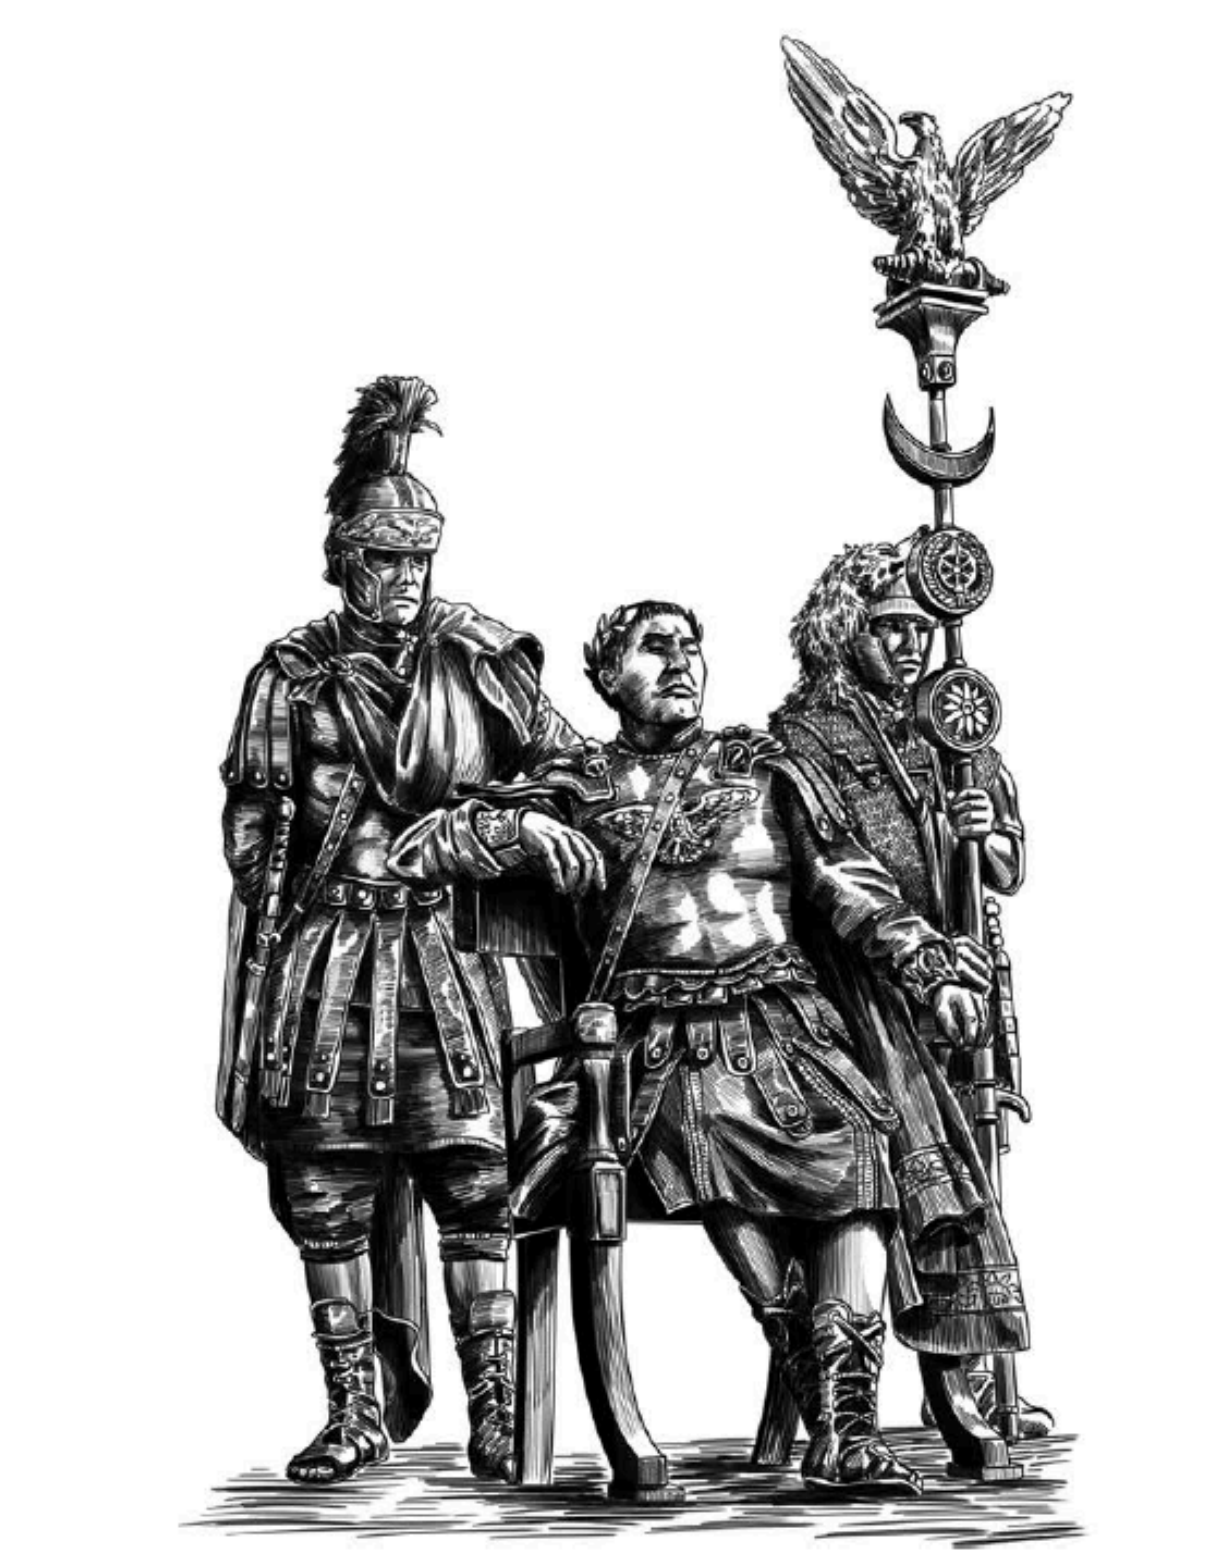
\includegraphics[width=0.5\textwidth]{assets/procurator.png}
    % \caption{The Procurator of Judea}
    \label{fig:pilate}
\end{figure}

So that's why he \emph{tried} to save Jesus. But why \emph{didn't} he? Why, after stating his premise (be it for reasons of state, to spite his enemies in the Sanhedrin, or simply on a lordly whim), did he not follow through to its conclusion and use his vast range of powers to their fullest extent? The standard version---``he chickened out because the local muckamucks threatened to snitch on him to the Dear Leader''---doesn't sound even remotely convincing. By that time, they had burned all possible bridges with the local authorities; a report here, a report there, what difference could it make?

Besides, an administrator as experienced as Pilate surely knew that such an accusation was never the actual reason for any punitive action; it could only ever be used as a formal pretext, if your fate was already sealed regardless. On the other hand, the procurator had already engaged in misconduct the moment he \emph{attempted} to exonerate a ``state criminal''; had this attempt been successful, that hardly would have mattered from the point of view of Tiberius' totalitarian regime (in the event they brought it to trial). Thus, so long as we assume that the driving force behind \emph{our} Pilate's actions were serious considerations of state, we can look at his ``about-face'' in that light as well.

Now, let us turn our attention to a rather significant detail, which for some reason, commentators on the Bible always seem to miss (or intentionally ignore). It is common knowledge that Christian tradition has done all it can to vindicate Pilate (in the Coptic and the Ethiopian Churches, he has even been canonized), laying all the blame for Christ's tragic death on the Jews. Meanwhile, in the time between Pilate's two ``not guilty'' verdicts, another was rendered: that of Herod Antipas, the Tetrarch (King) of Galilee. This detail, when considered with respect to the traditional view, is nothing short of outrageous. Let me explain.

As the representative of the semi-legitimate Idumean Dynasty, it was Herod, not the Sanhedrin, whose interests were most greatly affected by the crime Jesus was charged with---pretending to the Judean throne (``Are you the King of the Jews?''). Nevertheless, the Sanhedrin stubbornly insisted that Jesus be executed, and Herod, just like Pilate, saw absolutely nothing criminal in his actions. And this was the very same Herod who could be accused of everything except the ``idiotic disease of complacency'':\footnote{A phrase originating from one of Stalin's decrees, in which he alleged that several (mostly Jewish) doctors had conspired to assassinate government officials by way of ``negligence''; in context, it was used to lambaste the security services' purported inability to thwart the conspiracy. (Z.B.)} the platter with John the Baptist's head is more than enough evidence of that.

And in fact, no ruler, being of sound mind and body, would willingly prevent
the execution of a dubious prophet; either he is mad, or he is a rebel. As the khan
in \emph{The Enchanted Prince} tells his vizier in a similar situation:

\begin{smallquote}
    ``Once he has been seized and thrown into prison, why not cut his head off for safety's sake? We see no reasonable cause for abstaining! Revolt is much more serious than those Peshawar sorceries of yours, it is no joking matter!''\footnote{\emph{The Enchanted Prince}, Leonid Solovyov, trans. Bernard Isaacs, p. 167.}
\end{smallquote}

The explanation Christian commentators give for this usually runs along the lines of, ``Christ's innocence was so obvious that even a man as cruel and debauched as Herod could not uphold the Sanhedrin's verdict.''\footnote{ Universally Accessible Interpretation of the Gospel.} However, that is nothing more than childish prattle; in such situations, one's actual guilt or innocence means absolutely nothing. For Herod not to have subjected Jesus to the same \emph{Precautions} discussed by the aforementioned khan, he must have been under some degree of pressure, the source of which is quite obvious. Thus, Pilate's efforts to save Jesus must have been even more serious and sustained than the Gospel texts directly imply.

Herod's position (whether it was arrived at independently or by force), which is typically ignored as an insignificant detail, actually changes the picture of the balance of power quite radically. The image of an austere, honest Roman official, alone in his opposition to the Jews and their unshakeable religious fanaticism, disappears. In its place appear two supreme authorities---one Roman, one Jewish---who find themselves pestered by the ridiculous claims of one of the Judean public bodies. I should point out that the Sanhedrin functioned as not a criminal, but a purely religious tribunal, and the case they brought before Pilate was not even remotely within their jurisdiction. The Sanhedrin had full right to declare Christ a blasphemer and a heretic posing as the Son of God, and on those grounds they could sentence him to \emph{stoning} once they had submitted their---religious---verdict to the procurator for his purely formal approval.\footnote{ It was to stoning, the method of execution imposed for crimes against the Faith, that the high priest Ananus went on to sentence James, brother of Jesus several years later---without even bothering to inform the Roman procurator (Antiquities of the Jews, Book XX, 9:1). (K.E.)} Instead, with a persistence that remains completely incomprehensible, they slap the heretic Christ with trumped-up political charges and demand that Pilate \emph{crucify} him as a political criminal---a pretender to the Judean throne. As a result, the Sanhedrin, who have lacked the requisite authority from the very beginning, have moreover taken a legally indefensible position in their opposition to the secular authorities (namely, Pilate and Herod). And yet, at the very moment when it seems his opponent has no cards left to play, not even the very worst one, Pilate suddenly and inexplicably capitulates. What's the deal here?

The deal was that 23 relatively smart members of the Jewish clergy understood Christ's teachings just as well as Pilate did, and realized the threat posed by the young prophet's continued growth in popularity---both to the Temple of the Jewish faith and to them personally. And with that knowledge, they made a counterintuitive yet, as it turned out, perfectly calculated move: they arrested Jesus and came to Pilate with a blatantly illegal request---to execute him as a political criminal. This resulted in a magnificent ``fork'': either their hated rival would be liquidated at the hands of the Romans (with time, he could even be canonized asyet another hero who died at the occupiers' hands), or the procurator would let him go free, thereby acknowledging that the notorious Christ was a Roman ``agent of influence'' and rendering the prophet a political corpse.

There are serious grounds to believe that the Sanhedrin found the second option far more desirable, and more likely. Recall that if the high priests' only goal was to have Christ's head, then it would have been far simpler to go with the foolproof option of rendering a religious verdict. In any case, Pilate's approval of the execution of the ``King of the Jews'' clearly took them by surprise---kind of like someone who theatrically asks for his dismissal, then actually gets it. Only pure bewilderment could explain their panicked request for a Roman guard to patrol the burial site---this, in a city chock full of temple guards!

...The procurator realized he had lost: it was useless to keep up the fight for Jesus. Of course, he could simply pardon the Galilean, stamping a big fat X on his viability as a political figure, but that would just be pure capitulation. Nonetheless, he could still try to derive some benefit from the death of the popular prophet (as a benefit in this case meant anything to the Sanhedrin's detriment). And so, after making a show of washing his hands, Pilate---entirely of his own accord!---hands Jesus over to the soldiers for torture, then demonstrates to the crowd: it is the Sanhedrin that is guilty. From this moment on, the Sanhedrin will be guilty of everything, down to the gall and sour wine Christ is given by Roman soldiers (Mt 27:34). I've got to hand it to him---despite being down a piece, Pilate ultimately won the initiative and, to some extent, managed to equalize the game. The persistence and ingenuity of this ruthless chessmaster are certainly worthy of respect, but as for what could have possibly led anyone to canonize him, I admit I haven't the slightest idea.

But still, was there really no way for Pilate to even theoretically save Jesus, without ``outing'' him? Yes, there was---and he didn't hesitate to use it. ``At the feast the governor was accustomed to releasing to the multitude one prisoner whom they wished'' (Mt 27:15); so really, if the crowd in the square picked Jesus, the procurator could have released him without any problem, as there would be no sign of a ``Roman trail.'' But luck was not on his side; the crowd, of course, chose Barabbas---it would be strange if the high priests were careless and failed to ensure that the ``voice of the people'' was duly trained. However, this---completely natural---choice on the part of the Jews comes as a total surprise to Pilate. He repeats his request three times, entering into a pointless bickering match with the crowd that only leaves him further humiliated---in other words, he completely loses face.

So, the \emph{natural} course of events has clearly caught the procurator off guard. From this, it is logical to assume that there was some factor unknown to us (but known to the procurator) that was supposed to interfere with the natural course of events. \emph{Supposed} to, but didn't. The ``million dollar question'': what was this factor, and why didn't it work out as planned?
\chapter*[(First Warning to McDowell)]{Golgatha}

At this point, we are forced to start off with a theoretical digression---of the sort I have been trying my best to avoid. The deep, fundamental discrepancies between John's narrative on the one hand, and that of the Synoptic Evangelists on the other, are well-known (``How many gospels are there? Four? No: three and one'').\footnote{ Dmitry Merezhkovsky, \emph{Jesus the Unknown}, trans. H. Chrouschoff Matheson, p. 73. (Z.B.)} And Dmitry Merezhkovsky was probably right when he wrote that ``the dispute concerning John is the greatest enigma of Christianity... perhaps the enigma of Christ Himself.''\footnote{\emph{Jesus the Unknown}, p. 92.} To me, however---an irreligious person in general, and a complete virgin when it comes to theology---the coexistence of these two fundamentally irreducible and mutually irreconcilable versions seems perfectly normal and natural.

Strange as it may sound, it is actually my profession that has trained me to have such a perception. For us in the natural sciences, you see, knowledge is fundamentally reductive. Thus, as a rule, the continued coexistence of alternative conceptions of a natural phenomenon indicates that they are in fact complementary, and simply ``reduce'' observable reality to different aspects of its nature. As I see it, then, the opposition between John and the Synoptists is fundamentally no different from, say, the relationship between the wave and particle theories of light, which describe the same object in different ways, and only give an adequate impression of it when taken together as a pair. Again, let me quote from Merezhkovsky's apologia \emph{Jesus the Unknown} (pp. 97-98):

\begin{smallquote}
    John divines correctly---better perhaps than the synoptics---what Jesus \emph{intended}. What He \emph{did}, we learn from Mark; what He \emph{said}, from Matthew; what He \emph{felt}, from Luke. But what He \emph{intended}, we learn from John; and of course, it is what He intended that is of real, primary importance.\footnote{Emphasis Merezhkovsky's. (K.E.)}
\end{smallquote}

Now, that's all well and good on a general, conceptual level; in terms of the problem before us, though, where it is the specific details of the events that are important, the situation changes. We will frequently discover cases where John describes certain colorful incidents in detail that are completely absent from the Synoptists' narrative, and vice-versa---this is normal. In this sense, however, the scene at Golgotha is unique: here, the accounts of John and the Synoptists strike ``tit for tat,'' contradicting each other in literally every detail. And since my arguments are based on complete trust in the facts (though not necessarily their interpretations) reported by all four of the Evangelists, I find myself in a rather complex position, from which there is no clear way out.\footnote{However, one could still put forward the following hypothesis: the three Synoptic Gospels are genuine memoirs, whereas the Gospel of John was... let's say, a historical novel based on the others written many years later, in which truth and artistic license are melded into an inseparable whole. Furthermore, this second reality, owing to the genius (or Divine Inspiration, your choice) behind its creation, broke away, as one might expect, from its historical foundation and became entirely self-contained. I must admit that adopting such an assumption (which would allow me to disavow all of John's testimony) would make my life significantly easier. Alas! The starting conditions for the problem at hand (which include giving equal treatment to the four canonical texts) were defined quite strictly, and are not subject to review. (K.E.)}

% [htbp]: Instructs LaTeX to try placing the image Here, at the Top, Bottom, or on a separate Page (in that order).
\begin{figure}[htbp]
    \centering
    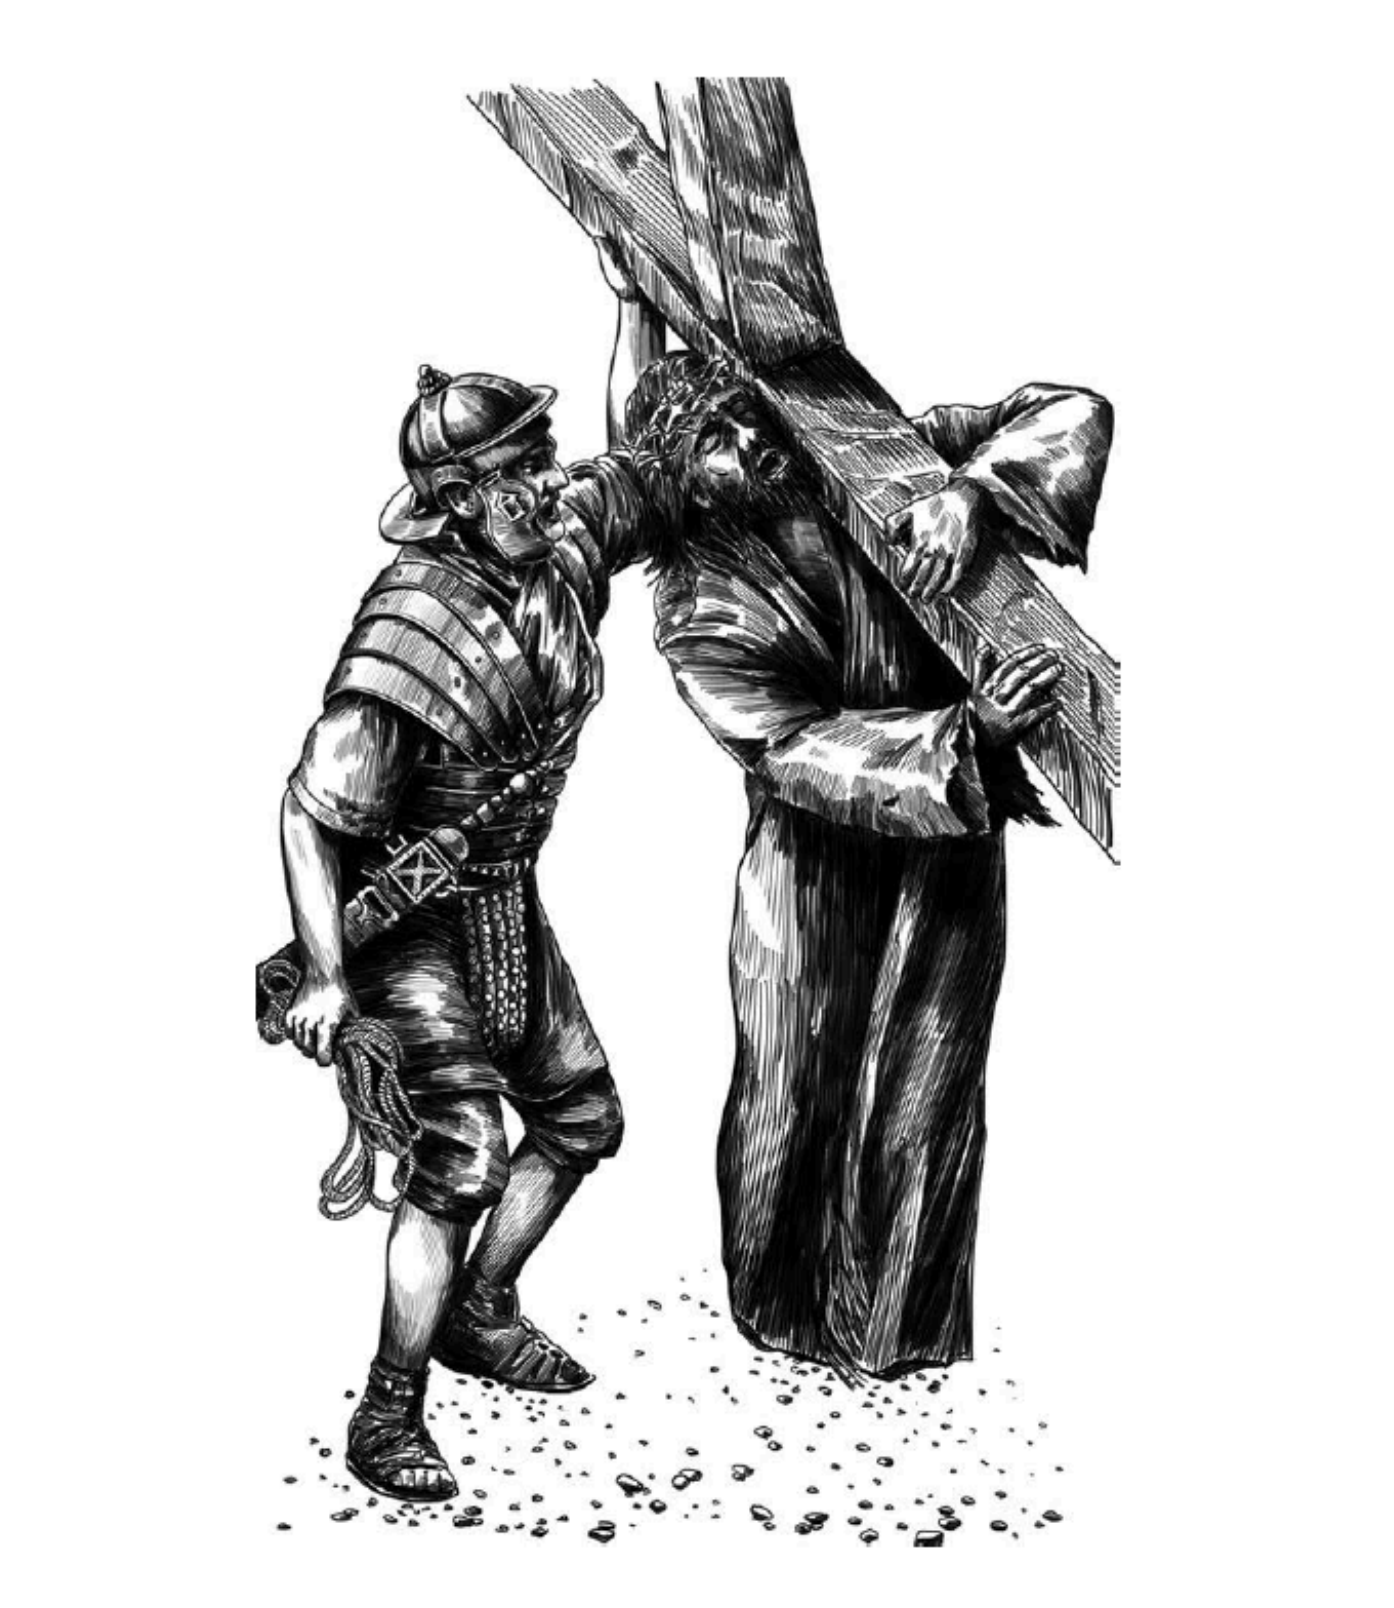
\includegraphics[width=1\textwidth]{assets/golgatha.png}
    \label{fig:golgatha}
\end{figure}

The discrepancies begin with a typical ``trifle.'' John confidently testifies that Jesus, ``bearing His cross, went out to a place called the Place of a Skull, which is called in Hebrew, Golgotha'' (Jn 19:17). Meanwhile, the Synoptists unanimously claim that the Savior's cross was carried by a certain Simon of Cyrene, and even include completely verifiable biographical details about the man, calling him ``the father of Alexander and Rufus'' (Mt 27:32, Mk 15:21, Lk 23:26). This time, you can't take lofty refuge in the nature of the Logos at hand, and you can't get out of this one with a casuistry like ``both of them are right, but each in their own way.'' You have to answer honestly: who got mixed up here?

I once heard the following, purely philological argument in support of the Gospels' authenticity as historical documents. It concerns a widely known episode:

\begin{smallquote}
    And about the ninth hour Jesus cried out with a loud voice, saying, ``Eli, Eli, lama sabachthani?'' that is, ``My God, My God, why have You forsaken Me?'' Some of those who stood there, when they heard that, said, ``This Man is calling for Elijah!'' Immediately one of them ran and took a sponge, filled it with sour wine and put it on a reed, and offered it to Him to drink. The rest said, ``Let Him alone; let us see if Elijah will come to save Him.'' (Mt 27:46-49)
\end{smallquote}

So (if I understand correctly), the use of unannotated direct speech to reveal the motivations of side characters only emerged as a literary device with the advent of the European psychological novel, in the 19\textsuperscript{th} century; therefore, what we are dealing with is the stenographically accurate record of an eyewitness. Perhaps this is because I am not a philologist, but this sounds completely convincing to me. However, I should point out that the argument refers specifically to the Synoptists' narrative---dry as a report, and therefore especially sorrowful. It is in their account that a Man dies betrayed and abandoned by all those around him---a far cry from the figures of chromium-molybdenum steel who feature in \emph{Lives of the Saints}.

In the Gospel of John, of course, these words are nowhere to be found. On the other hand, you find, for example, a quotation from Jewish scripture that Roman soldiers casually recite verbatim (Jn 19:24)---just in case the people around them fail to notice that they are not merely casting lots for a dead man's clothes, but fulfilling an ancient prophecy? There is also the sublime conversation that a dying man, suffering the most terrible of agonies, carries on with the people standing at his cross: his mother and the ``disciple whom he loved,'' that is, John (Jn
19:26-27).\footnote{McDowell provides a detailed description of the medical aspects of crucifixion. It is often believed that death results from shock, combined with dehydration and heatstroke, but that is actually somewhat inaccurate. Several hours after crucifixion, a person starts to develop pulmonary edema due to the difficulty in breathing; the immediate cause of death is asphyxiation. Hence, a person undergoing crucifixion is incapable of holding an extended, coherent conversation as a matter of principle. (K.E.)}

Wait a second! Among other things, the Synoptists have neither his mother nor his disciple there at all. The only ones there are the Galilean women who follow Christ everywhere---Mary Magdalene, Mary, mother of James, and Salome---and they are not standing anywhere near the cross, but are looking on \emph{from a distance} (Mk 15:40, Mt 27:55). How could it be that all three Synoptists failed to notice such a ``small detail'' as John and the Virgin Mary \emph{standing at the cross}? Especially since Ivan Bezdomny's vision of Bald Mountain quite inaptly springs to mind: ``and the mountain was encircled by a double cordon.''\footnote{\emph{The Master and Margarita}, p. 143.} Of course, you could hardly call that authoritative---and yet... I honestly admit that I have no idea what to do here---unless I adopt Merezhkovsky's interpretation and come to the straightforward, yet depressing conclusion that the Savior merely \emph{wanted} his mother and his beloved disciple at his cross...

Where am I going with this? Well, taking on the role of counterintelligence agent Philip Rawlings, who ``doesn't believe anything he hears, and very little of what he sees,''\footnote{Ernest Hemingway, \emph{The Fifth Column and Four Stories of the Spanish Civil War}, p. 27} I just can't help but wonder: was the man who was crucified between two robbers at noon on the fourteenth day of the spring month of Nisan\footnote{This specific phrasing for the date of Jesus' death is used several times throughout \emph{The Master and Margarita} (e.g. p. 13, p. 255). (Z.B.)} really the same man who, six days before, had entered Jerusalem to the cheers of ``Hosanna''? If the conversation with his mother and disciple really took place the way John reported it, then yes, absolutely. But if nothing took place on Golgotha other than what the Synoptists so meticulously described, then I'm sorry, but just about anybody could have been hanging on the middle cross---perhaps a robber just like the two others, or perhaps a Zealot partisan.

One need only assume that, for their own benefit, the Roman authorities wanted to strengthen the position of Jesus' sect, and that he made a deal with them (``the end justifies the means'')---and there would be practically nothing left unclear in the entire story of the Resurrection. This, incidentally, would explain the role of the episode where Jesus is dressed in a scarlet military cloak---after his trial, but before his scourging and his ascent of Golgotha (for example, Mk 15:17-20). After the scourging, they put Jesus' clothes on another man---the man who was to take his place on the middle cross.

Personally, I don't intend on defending this theory, or even seriously analyzing it, as that would force me to reject the ``presumption of honesty'' that I am obliged to uphold (in accordance with the starting conditions). But while I have the right to make such a ``withdrawal,'' McDowell does not. And considering that he took the time to craft a completely serious argument against the \emph{Passover Plot} hypothesis, where not a single fact adds up, and Christ and Joseph of Arimathea cheat side-by-side like a pair of train station cardsharps, he is simply obliged to examine a hypothesis as patently obvious as the ``Uncrucified Christ.''

At the same time, however, by no means do I wish to say that McDowell's position on that issue would be indefensible. He could most likely cite the high priests who visited the execution site (Mt 27:41) or the conversation with the remorseful robber: ``Assuredly, I say to you, today you will be with Me in Paradise'' (Lk 23:43). In turn, an ardent supporter of this hypothesis could object that the face of the man on the cross was disfigured beyond all recognition in any case; that the high priests certainly did not come up close to the cross, and a person undergoing crucifixion (assuming it takes place not in a classical painting, but in real life) is forced to keep their face lowered to the ground; that the organizers of the hoax surely would have taken care to increase the physical resemblance of the people involved; that the conversation with the robber could not have been heard by anyone apart from the legionnaires, and their ``testimony'' is clearly worthless, etc. In short, both sides would have wide room to maneuver here.

However, the problem lies not in these particularities. Even if McDowell manages to provide a sufficiently convincing rebuttal of the ``Uncrucified Christ'' hypothesis, his position will not become any less unenviable. After all, his entire \emph{system} of proof is based on the assumption that he has analyzed (and refuted) \emph{every} possible materialist theory---and suddenly, a special case pops up... It just goes to show that the range of logical possibilities is fundamentally inexhaustible, and there's nothing you can do about it.

In short, it seems that McDowell's dreadnought has already struck a sea mine on its way out of the harbor. And while the crew's efforts might keep the ship afloat, its use as a combat unit will be rather limited from here on out. However, there are even greater surprises in store for Captain McDowell on this voyage...
\chapter*{John the Baptist}

Let us return now to the very beginning of Jesus Christ's public ministry, when fate brought him face-to-face with the last of the Old Testament prophets, John the Baptist. The Forerunner of the Savior (``He who is coming after me is mightier than I''---Mt 3:11), who considered himself ``not worthy to loose His sandal strap'' (Jn 1:27), John was the first to correctly recognize the divine essence of Jesus: ``Behold! The Lamb of God who takes away the sin of the world!'' (Jn 1:29). A man who sharply rebuked both religious and secular leaders (``Brood of vipers! Who warned you to flee from the wrath to come?''---Mt 3:7), he paid with his life for his denunciation of the lawlessness and debauchery that Herod, the tetrarch of Galilee, was mired in. At first glance, this personage (whose historicity, incidentally, is without question) seems to have absolutely no mystery about him. However, let us conduct a careful and impartial analysis of John's relationships---first, with Jesus, and second, with the authorities (in particular, Herod Antipas).

The first (and last) meeting between Jesus and John took place on the banks of the River Jordan, in whose waters the prophet would baptize the crowds of people who flocked to him. Jesus, among others, asked to be baptized; John ``would have prevented him, saying, `I need to be baptized by You, and are You coming to me?''' (Mt 3:14). The moment the ritual was performed, the Holy Spirit descended upon Jesus in the form of a dove (visible only to the Baptist, however). The episode of the baptism is described practically identically by all four Evangelists, but afterwards, like usual, significant discrepancies begin to emerge between John and the Synoptists.

John the Evangelist writes that the next day, John the Baptist sent Jesus adetachment of two of his own novices---Andrew and another not mentioned by name---who became his first disciples. Later on, Jesus and his newly formed community returned to Galilee, where he performed his first miracles. Then, he went on his first Passover pilgrimage to Jerusalem; there, he expelled the money changers from the Temple for the first time, and also held a nighttime conversation with a member of the Sanhedrin named Nicodemus. After this:

\begin{smallquote}
    Jesus and his disciples came into the land of Judea, and there He remained with them and baptized. Now John also was baptizing in Aenon near Salim, [...] \emph{for John had not yet been thrown into prison}'' (Jn 3:22-24).
\end{smallquote}
Let's keep this last phrase in the back of our minds; it is very important.

Since by this point, more people were coming to Jesus to get baptized than
to John, the latter's disciples voiced their resentment at the success of their ``rival." John, however, admonished them for their jealousy, comparing Jesus to a bridegroom, and himself to the best man, who must not envy his friend, but feel happy for him (``He must increase, but I must decrease''---Jn 3:30). Following this, all references to John the Baptist in the Gospel of John disappear.

Now, let us return to the phrase ``for John had not yet been thrown into prison.'' Given that it appears in the chronologically last of the four Gospels, it comes across as a direct objection to the Synoptists' version, and an attempt to remind them of how things really were. After all, if you believe the Synoptists, Jesus retreated into the desert immediately after his baptism to pray and overcome temptation; it was there that he learned of John's arrest (Mt 4:12, Mk 1:14). Only \emph{after} he received this news did he travel to Galilee, and only \emph{there} did he gain his first disciples, Andrew and Simon---fishermen on the Sea of Galilee. The importance of this seemingly insignificant detail---when precisely the Baptist was arrested---becomes clear from the subsequent narrative of the Sypnotists

Matthew and Luke go on to recount the so-called ``Embassy from John the Baptist''; after hearing of the miracles Jesus has performed, the prophet sends two of his disciples to him to investigate:

\begin{smallquote}
    ``Are You the Coming One, or do we look for another?'' Jesus answered and said to them, ``Go and tell John the things which you hear and see: The blind see and the lame walk; the lepers are cleansed and the deaf hear; the dead are raised up and the poor have the gospel preached to them.'' (Mt 11:3-5)
\end{smallquote}
After John's disciples depart, Jesus delivers a panegyric in honor of his Forerunner:

\begin{smallquote}
    ``Assuredly, I say to you, among those born of women there has not risen one greater than John the Baptist. [...] And if you are willing to receive it, he is Elijah who is to come'' (Mt 11:11-14).
\end{smallquote}

When you really think about it, this episode contradicts the entirety of the
narrative preceding it. It's bad enough that the \emph{Forerunner} is continuing his
ministry alongside the Lamb of God, who has \emph{already come} into this world. That
aside: if you have any grounds to believe that the Messiah has arrived, then surely
your first instinct would be to go see him yourself, and not send your disciples to
check things out. However, the Synoptists already have this question covered: the
only reason John the Baptist didn't come in person was because he was in prison at
the time (Mt 11:2), having been arrested almost immediately after Jesus' baptism.

But then John snaps back: nothing of the sort---the Baptist was still a free man for quite some time afterwards, and was performing baptisms side-by-side with Jesus. It seems the Evangelist understood the true meaning of this episode far better than the Synoptists did, for which reason he deliberately excluded it from his narrative---as this episode makes it abundantly clear that even in the best case scenario, the Forerunner had his doubts as to whether Jesus really was He who would ``baptize with the Holy Spirit and fire'' (Lk 3:16). What's more, the Synoptists are completely silent as to how John reacted to his ambassadors' report. If that's the case, then what to make of everything John said upon meeting him personally (``Lamb of God,'' ``you come to be baptized by me?''), or the sign given directly to John in the form of a dove? Incidentally, I should point out that the entire scene of the baptism (as well as John's subsequent ``exhortation on Christ''---Jn 3:22-36) is what is known in legal terms as ``hearsay,'' as none of the Evangelists were personally there to witness it.

If you objectively analyze everything John said (and even more so, did), you inevitably arrive at a discouraging conclusion: at no point did the Forerunner clearly and unequivocally recognize his distant relative (according to Luke) as He who ``would come after him more powerful than he.'' Several of the Baptist's statements regarding Jesus (for example, ``and no one receives His testimony''---Jn 3:32) have forced Christian commentators to resort to plaintive explanations such as, ``The Evangelist didn't quite accurately convey the prophet's meaning...'' If we so desired, we could easily read some episodes differently from the way they are typically interpreted.

Take, for example, how Gladkov describes the scene of the baptism:
\begin{smallquote}
    Recognizing that John had been sent by God to baptize, Jesus, a Man who had heretofore fulfilled all the Lord's commandments, began His ministry by fulfilling the last Old Testament commandment, which God had just announced through John. \emph{As He was without sin, He had no need to repent, for which reason he petitioned John directly to baptize Him} [emphasis mine---K.E.]. John saw at once that this was no ordinary man standing before him, and thus replied: ``I need to be baptized by you, and do you come to me?''
\end{smallquote}

Now here's how \emph{I} imagine this scene might have played out. Before this supremely authoritative prophet, who fills the Pharisees and Sadducees with awe and regularly sermonizes to enormous crowds of people, appears a young man who no one has ever seen before. He announces that since he is without sin, the only thing he needs from him is to be baptized. John, utterly astonished at such (from his perspective) insolence, throws up his hands with feigned humility. ``Guess you're right, buddy, you've come to the wrong guy. You know what, \emph{I} shouldn't be the one baptizing \emph{you}---\emph{you} should be the one baptizing \emph{me}!'' The audience is delighted---he sure showed him!

Christian commentators often claim that John himself directed his crowds of followers to Jesus; however, this is completely unsupported by the Gospel texts. It's possible some members of John's community actually did leave him for Jesus (Christ would go on to see many of his disciples leave him as well---a common occurrence), but this migration was clearly neither organized nor widespread. John the Evangelist's account of the Baptist ``gifting'' Jesus his first disciples, as we may recall, is unanimously contradicted by the Synoptists. A rather telling detail: after John's execution, his disciples made a special trip to tell Christ the news (Mt 14:12), but not one of them ended up joining his community!

The desire of John's disciples to stick by their teacher's side, especially during the trying times of his imprisonment, deserves nothing but respect. But then came John's demise; it would seem only natural for them to start following the man who their dearly beloved teacher (as the Evangelists tell us) deemed himself the forerunner to. Yet nothing of the sort ever happened. In fact, the Johannites maintain a separate identity from Christians to this very day, existing in the form of a Jewish sect; they have a ``Sacred Scripture'' of their own where John the Baptist is recognized as the Messiah, while Jesus is taken to be a false prophet. And when you really think about it, this is all perfectly natural. How do you think John---a somber, puritanical Jew---would take to a man who miraculously turned water into wine for partygoers and rubbed shoulders with prostitutes, tax collectors, and occasionally---perish the thought!---uncircumcised gentiles?

And so, we observe a rather pronounced asymmetry in opinion: for Christians, John is their greatest prophet and a highly revered figure in general, whereas for the Johannites, Jesus is a false messiah. In addition, there are no grounds to believe that each of these sects formed their opinions \emph{in spite of} the statements of their founders. For this reason, the Evangelists were faced with an intractable problem when it came time to describe these events. On the one hand, Jesus Christ, the Son of God, whose every word is Truth incarnate, had a very high opinion of John the Baptist (something they witnessed directly); on the other hand, said John, as far as they knew, did not return his feelings and was not particularly fond of their teacher. How could they possibly resolve such a contradiction?

Here's how: by taking the many statements of John the Baptist (both authentic ones and those attributed to him by rumor) and selecting only those that could point to him recognizing the divinity of the Evangelists' teacher. The lack of written texts made this task significantly easier. More likely than not, many of the statements attributed to John probably originated among Jesus' followers themselves. After circulating among the population at large (and gathering new ``details'' along the way), these stories later returned to the Evangelists, who gladly recorded them as ``independent testimony''---a well-known effect in sociology. The ``beloved disciple''---the author of the fourth gospel, John---went further down this path than the others did. Not only did he introduce the apocryphal episodes of Christ being ``gifted'' his first disciples and the ``exhortation on Christ'' (neither of which appear in the Synoptic Gospels), he also omitted such obvious kompromat as the mention of his teacher's ``inspection'' by the Baptist's disciples (which, on the contrary, he was certainly a witness to---along with the other Apostles).

So were the Evangelists deliberately trying to bolster their teacher's reputation by invoking the opinion of an authoritative independent source---modifying the latter's actual statements in order to suit their needs? No, no, and no! Any believer knows full well that Christ's authority---in the eyes of the Apostles---needed no ``independent testimony'' whatsoever to support it. For this reason, I am absolutely convinced that the Evangelists' correction of the Baptist's statements was a genuine attempt to save \emph{his} authority---the authority of a man who, for some reason, hesitated to recognize the patently obvious fact that Jesus was the Messiah. And needless to say, the Evangelists' efforts paid off; they literally created the John the Baptist who lives in our consciousness to this very day. The actual John, as I strongly suspect, would have justly occupied a place, if not alongside the Pharisees and other ``Jewish elders,'' then in any case very far away from the Son of Man.

Moving on to an analysis of John the Baptist's relationship with the secular authorities, we need to make one caveat. The Evangelists only knew the details of the prophet's tragic death through hearsay, just like any other citizen of Palestine who wasn't one of Herod's courtiers or a member of his secret police force. For this reason, the testimony of the New Testament texts will not be given any inherent precedence over that of Josephus' \emph{Antiquities}. Let us recall that \emph {Antiquities} is the only non-Christian source that directly mentions such figures from the Gospel as John the Baptist and James, the brother of Jesus. As a result, the Church treats Josephus' testimony with a high degree of reverence; in particular, it is from this source that the Baptist's place of captivity, the fortress of Machaerus,\footnote{``John the Baptist,'' Bible Encyclopedia, II:91-92.} is taken.

Mark the Evangelist (Mk 6:17-29) describes the prophet's death as follows. John, in spite of his imprisonment, continued to maintain his influence over Herod:

\begin{smallquote}
    Herod feared John, knowing that he was a just and holy man, and he protected him. And when he heard him, he did many things, and heard him gladly.
\end{smallquote}
The prophet, among other things, kept insisting that the tetrarch break off his relationship with Herodias, whom he married after divorcing his previous wife (the daughter of the Arab king Aretas IV) and dissolving the marriage of his brother Philip:
\begin{smallquote}
    Because John had said to Herod, ``It is not lawful for you to have your brother's wife.'' Therefore Herodias held it against him and wanted to kill him, but she could not.
\end{smallquote}

The opportunity presented itself at a feast, when Herodias' daughter Salome left Herod so stunned by her dancing that he quite simply went insane:

\begin{smallquote}
    He also swore to her, ``Whatever you ask me, I will give you, up to half my kingdom.''
\end{smallquote}
Uninterested in half of his kingdom, the princess, at her demonic mother's instigation, asked the king for the head of his irksome reproacher:

\begin{smallquote}
    And the king was exceedingly sorry; yet, because of the oaths and because of those who sat with him, he did not want to refuse her.
\end{smallquote}
One of his henchmen was dispatched to the prison, and several minutes later, he presented the bloodthirsty beauties a platter with the prophet's severed head. And small wonder: woman, of course, is the root of all evil, and truly is she said to be ``the devil's gateway''\footnote{Tertullian, \emph{On the Apparel of Women}, trans. Sydney Thelwall, Book 1, Chapter 1.} (and if you have any doubts, take another look at Oscar Wilde's \emph{Salome}).

Josephus, meanwhile, tells a different, far more prosaic story:

\begin{smallquote}
    Now when [many] others came in crowds about [John]; for they were very greatly moved [or pleased] by hearing his words; Herod, who feared lest the great influence John had over the people might put it into his power and inclination to raise rebellion... thought it best, by putting him to death, to prevent any mischief he might cause; and not bring himself into difficulties by sparing a man who might make him repent of it when it would be too late. Accordingly he was sent a prisoner, out of Herod's suspicious temper, to Macherus; the castle I before mentioned; and was there put to death. Now the Jews had an opinion, that the destruction of this army [in the war with Aretas] was sent as a punishment upon Herod; and a mark of God's displeasure to him.\footnote{\emph{Antiquities of the Jews}, Book XVIII, Chapter 5.}
\end{smallquote}
So, there were no personal motivations at work here---it was politics all the way down. In comparing these two versions, let us first turn to the factual side of the matter---specifically, everything we know about the marriage of Herod Antipas and Herodias.

% [htbp]: Instructs LaTeX to try placing the image Here, at the Top, Bottom, or on a separate Page (in that order).
\begin{figure}[htbp]
    \centering
    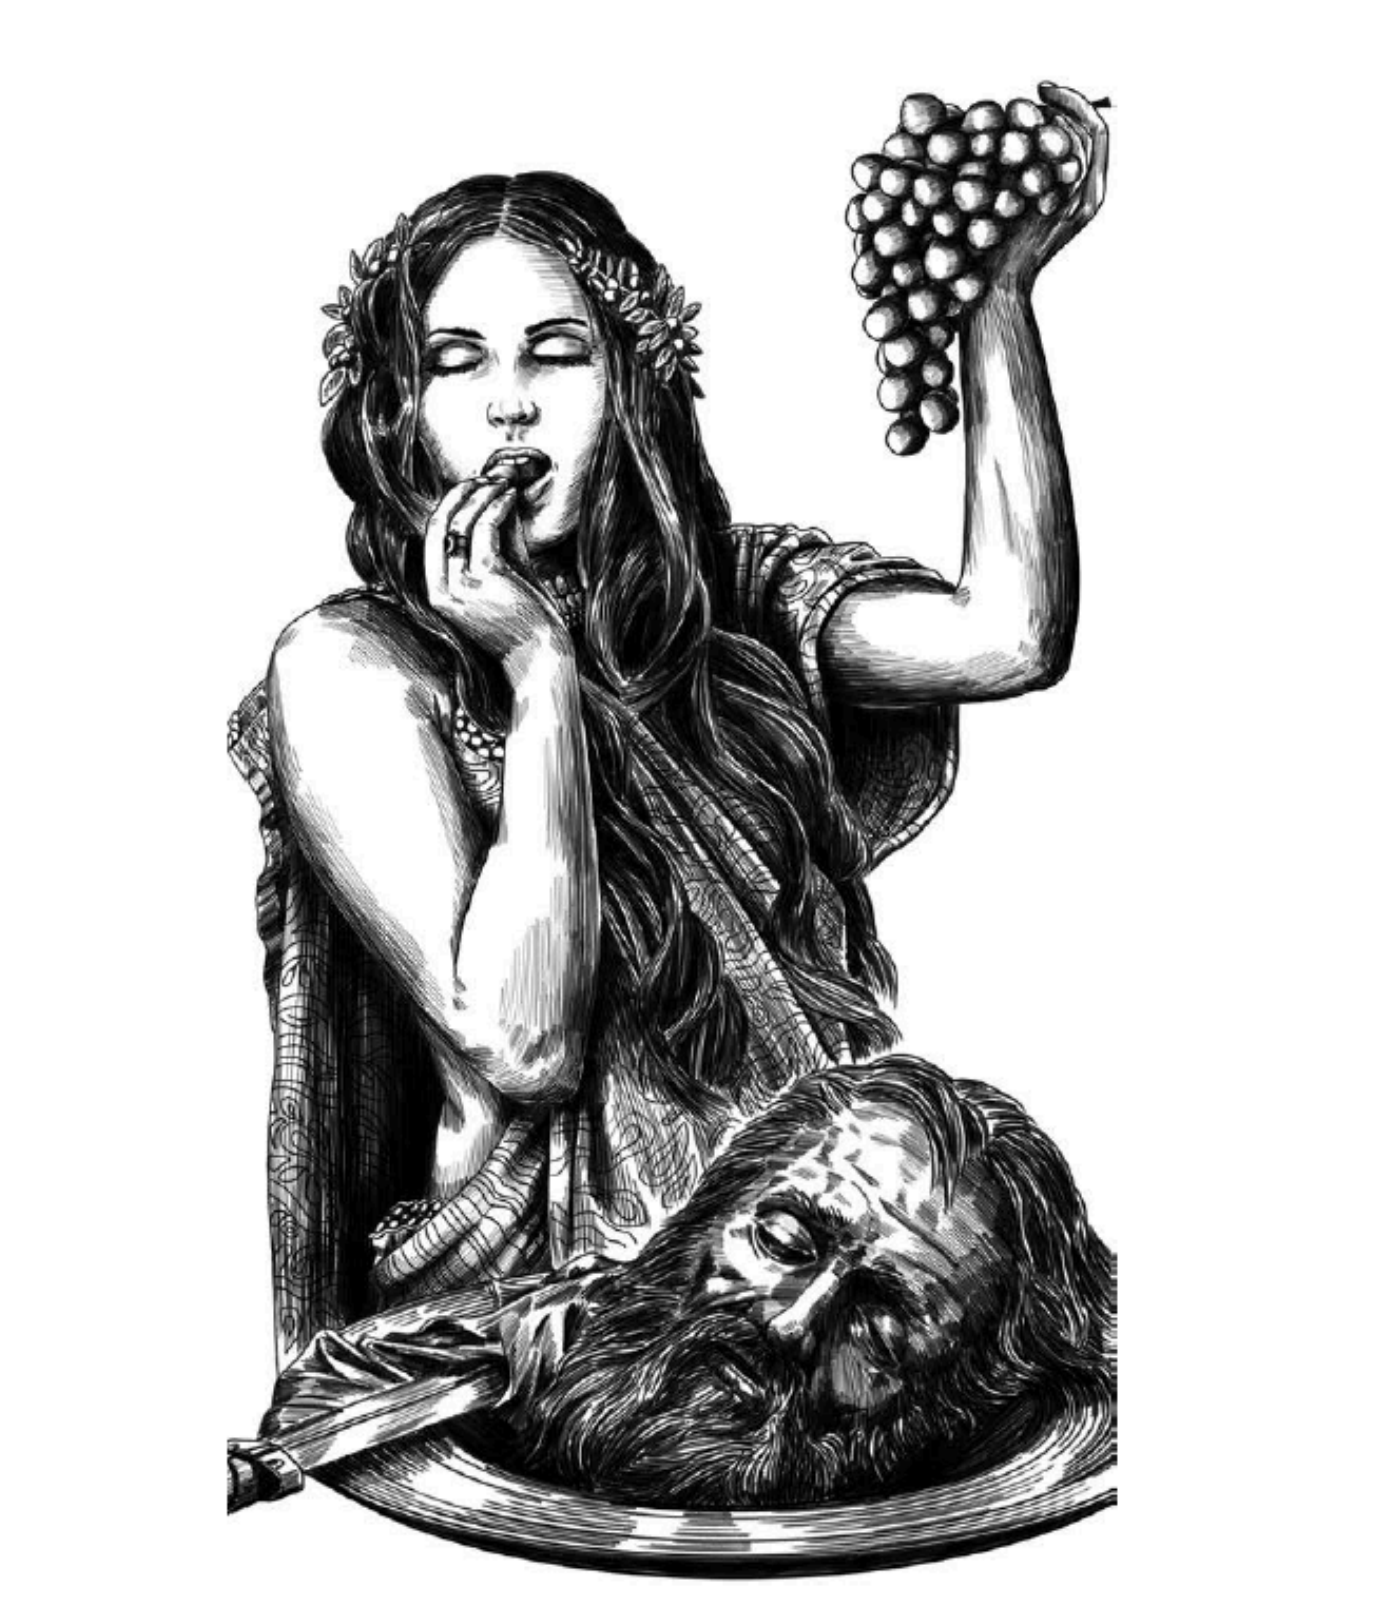
\includegraphics[width=1\textwidth]{assets/john-the-baptist.png}
    \label{fig:john-the-baptist}
\end{figure}

\newpage
First, what was the nature of Herod's previous, dissolved marriage? Let's give the floor to Metropolitan Joseph, commentator on \emph{Antiquities}:

\begin{smallquote}
    With his tetrarchy sharing a border with such longtime predators as the Arabs, Antipas greatly facilitated the security of his subjects by building new military fortifications in the outskirts of the country. And not for nothing is his very marriage to the daughter of the Arabian king Aretas suspected to have been an act of pure political calculation, which would serve to ensure peace for his country better than any fortresses or weaponry could, assuming the marriage was not imposed upon him by Augustus.\footnote{\emph{The History of the Jewish People According to Flavius Josephus' Antiquities}, book III, chapter VII.}
\end{smallquote}
The dissolution of this forced, dynastic marital union---at his wife's initiative, no less---resulted in Herod's ill-fated border war with Aretas, but that's a whole other story.

Second, Herodias was previously the wife of Herod's stepbrother, not his biological one (as is commonly thought); the aforementioned Metropolitan Joseph provides ample evidence for this fact. It's not at all surprising that Josephus' account presents this as a completely ordinary story of a second marriage; in general, the Jews saw marriage not as a sacrament, but as a civil status, so divorce was an extremely common occurrence. I should note that Josephus himself was a member of the Pharisees, who were renowned for their expert knowledge in Mosaic Law; moreover, he had no warm feelings for the hellenized Herod. You would think that he, out of all people, would waste no opportunity to take yet another dig at the worthy offspring of Herod the Bloody---assuming there was anything even remotely criminal about the affair.

Third, Herodias has always been seen as a calculating seductress, who not only broke all laws of marriage just to wrap the king of Galilee around her finger, but then, toying with an ax, kept a watchful eye on her cozy perch by the throne. And again, that doesn't track. Several years later, the emperor Caligula ordered, so to speak, the ``dismissal of Mr. Antipas, Tetrarch of Galilee and Perea, from his present position due to his inability to fulfill his duty,'' and exiled him to Spain, where he ultimately died---in poverty, obscurity, and total isolation. The only person who shared his exile with him, up until his dying day, was Herodias. It makes me wonder: would a woman like that really care what some scruffy, unwashed puritan was shouting about her ``family values''?

And now, the actual episode of John's beheading. Let's start off with a seemingly basic question: where did it take place? Well, the king is celebrating his birthday with his courtiers, military commanders, and elders; in light of the absence of any specific indications in the text, it would be logical to assume that the feast was held at its typical location---Herod's palace at Tiberias, on the Sea of Galilee. But during that time, John was held captive at the fortress of Machaerus (or Macheron), which is on the Dead Sea---and this comes from the same testimony by Josephus that the Church takes as fact! It should be noted that the Evangelists' account states that Herod did not merely give the order to execute John the Baptist (for which purpose he could have sent messengers from Tiberias to Machaerus, about 60 kilometers as the crow flies); no, right then and there, after several minutes had passed, he presented his stepdaughter the platter with the prophet's severed head.

In trying to resolve this obvious contradiction, some Christian commentators have tried---completely arbitrarily---to move the scene's location to Machaerus (if the mountain won't come to Muhammad, then Muhammad must go to the mountain). Gladkov, for example, goes so far as to tie this to political events:

\begin{smallquote}
    Insulted [due to his daughter's divorce---K.E.], Aretas started a war against Herod; as a consequence of this, Herod and his entire court moved to Machaerus, where he had imprisoned John the Baptist, and took up residency in his palace there.
\end{smallquote}
Well, let's start with the fact that Macherus was a small border outpost in the outskirts of the Arabian desert, and needless to say, there were no palaces there to speak of. Only recently, at the start of the protracted border war between Herod and Aretas, had the Jews captured the fortress from the Arabs, who had controlled it in previous years. Pretty strange idea to go to a place like that for your birthday, don't you think? Not to mention---what king brings his entire court, including his wife and children, out to an \emph{active war zone}?

Or consider this detail: after Herod's ill-advised promise, Salome ``went out and said to her mother, `What shall I ask?' And she said, `The head of John the Baptist!' Immediately she came in with haste to the king and asked, saying, `I want you to give me at once the head of John the Baptist on a platter''' (Mk 6:24-25). Well, I'll be... I guess the princess put on a striptease for her stepfather's drunken guests just for the hell of it, with no concrete goal in mind beforehand?

For these reasons, I cannot help but be extremely skeptical of the Evangelists' version of the events. From an artistic perspective, though, the story is truly magnificent. It manages to organically combine obvious folklore elements (``Even if you ask for half my kingdom!'') with a tightly structured plot---and just by itself, the semantic hieroglyph of the ``head on a platter'' provides ample fodder for pretentious art critics and psychoanalysts! Of course, to preserve the dynamism of the action (the immediate fulfillment of Herod's rash promise), it was necessary to sacrifice some degree of accuracy and move John to Tiberias (or alternatively, Herod to Machaerus), but such a sacrifice seems fully justified. It seems highly improbable that such a plot could spontaneously ``clump together'' from the various rumors circulating about the death of the popular prophet.

All of this allows me to make the following conjecture: this rumor about the circumstances of John the Baptist's demise, which the Evangelists Mark and Matthew faithfully reproduced in their respective Gospels, was the result of an ``active measures'' campaign.\footnote{A contemporary term referring to the practice of influencing public opinion through channels of official propaganda. A classical example of ``active measures'' is described in Leonid Solovyov's \emph{The Tale of Hodja Nasreddin}, where undercover guards in teahouses and caravanserais try to convince the people of Bukhara that their beloved Hodja has been a longtime servant of the emir. A more recent example is the use of KGB-controlled newspapers (mainly in third-world countries) to disseminate stories claiming that the AIDS virus was created in a Pentagon laboratory (see \emph{KGB: The Inside Story of Its Foreign Operations from Lenin to Gorbachev} by Christopher Andrew and Oleg Gordievsky, pp. 529-530). (K.E.)} Its goal seems quite obvious: to shift a significant portion of the blame away from Herod (who supposedly ``did many things when he heard John, and heard him gladly''), depicting the tetrarch as the naive victim of perennial feminine guile. Who, then, was the initiator of this (judging from its result) exceptionally competent campaign to shape the public opinion of Palestine?

The answer, as I see it, will emerge of its own accord when we can successfully answer another question, closely tied to the first: who arrested John the Baptist? Right now, the reader is probably looking at me like I'm a total idiot---after all, the Evangelists and Josephus seem to be in complete agreement on this point. So let me refine the question a little: let's suppose it really was Herod who \emph{executed} John. But who \emph{carried out the arrest}, and on what grounds? The Gospel texts lack any concrete indications in this regard; what's more, the situation here is nowhere near as simple as it first appears, and here's why.

The problem is that John was a native of Judea, and lived there his whole life. He led an ascetic existence preaching in the Judean desert and the Jordan River Valley near Bethabara and Aenon. At times, he would travel to the left bank of the Jordan in Perea, but by all accounts, he never spent any time in Galilee. Therefore, John's preaching should really have only been a headache for the Judean high priests and procurator---not Herod. Moreover, the Judean leadership was actually quite sympathetic to the prophet (at least in the beginning), and many Pharisees and Sadducees even sought to be baptized by him (Mt 3:7).

Furthermore, if the tetrarch of Galilee wanted to get his hands on the scandalous preacher, it wouldn't be too easy to do; Judea was in at least some sense a foreign country, and the relationship between the Judean and Galilean authorities left much to be desired. But perhaps John, for reasons unknown to us, left Herod so upset by his preaching that he decided to thumb his nose at both the law and common courtesy, and send an arrest team into foreign territory?\footnote{Anyone who believes that the extraterritorial ``actions'' of the NKVD, whose victims included Alexander Kutepov, Leon Trotsky, and countless other Russian emigres, were an unprecedented event in world history, is sorely mistaken. The secret services of civilized and democratic France, for example, took great pleasure in kidnapping and killing OAS agents who had fled across the border, paying no heed to the protests of their neighbors---carrying on a proud tradition that started with the abduction of the Duke of Enghien by Napoleon's gendarmes. (K.E.)}

While we can't rule out this possibility, it would render Christ's reaction to this event utterly incomprehensible, considering that he was also in Judea at the time: ``Now when Jesus heard that John had been put in prison, He departed \emph{to Galilee}'' (Mt 4:12).

So, let's try to sum up everything we've established so far. First, a rather popular and influential spiritual leader was preaching in Palestine at the same time as Jesus Christ. Second, his relationship to the Son of Man was apparently not as idyllic as is commonly believed. Third, the death of said leader took place in highly unclear circumstances, the nature of which I suggest we ought to reflect on.
\newpage
\begin{center}
    \Huge The Raising of Lazarus 
\end{center}

Now let's turn our focus to the event that immediately preceded Holy Week and, in a certain sense, served as the start of the tragedy---namely, the Raising of Lazarus. It was following this event that the high priests realized that the popularity of this new prophet and miracle worker had risen to dangerous levels, and it was time to take serious action. And it was at that moment that fate, as if on cue, sent them a priceless gift, the defector Judas; life abounds with such coincidences...

Of all the miracles performed by Christ, the Raising of Lazarus really does stand alone. Non-traditional commentators on the Gospel have quite rightly observed that almost all the people Christ healed were suffering from psychological or psychosomatic disorders. These included various types of paralysis and blindness, epilepsy, and (in the case of Jairus' daughter) lethargic sleep; in the case of the lepers, they might actually have been suffering from severe, untreated eczema. It is a well-known fact that such disorders can actually be cured by the power of suggestion. Jesus' outstanding talent for suggestion is clearly demonstrated by another set of miracles, such as feeding a crowd with five loaves of bread and two fish, turning water into wine, or walking on water, all of which can easily be interpreted as cases of mass hypnosis. For obvious reasons, however, the Raising of Lazarus---a man who had died several days earlier, had already been entombed, and was ostensibly starting to decompose---defies all possible explanation from a materialist standpoint.

Now of course, we could still ``stick to our guns'' here and come up with a pseudo-materialist hypothesis to explain this. There are many documented cases of people being ``revived'' after spending an extended amount of time in a state of ``quasi-death'' (where a person's metabolic rate falls to an imperceptible level, and they lack any visible signs of life, such as a pulse). First are Indian yogis, who are able to enter and exit such a state at will, as well as spend several hours underwater, or more than a day under a layer of earth. Second are the more interesting (from our case's perspective) zombies,\footnote{In recent years, American journalists have come to use the word ``zombie'' in a looser sense, to describe people who have intentionally been subjected to mind-altering substances, hypnosis, and so on, with the goal of manipulating their behavior. Widely-known examples of this include the experiments conducted as part of the CIA research programs ARTICHOKE and MKUltra, which became the subject of a Senate investigation. Here, however, we are using the term ``zombie'' in the original sense of the word---the same way it is used in black voodoo cults in West Africa and the Antilles. (K.E.)} who are temporarily put into such a state by a sorcerer; he then passes them off to his fellow tribesmen as corpses that have been ``revived'' by the power of his magic. In recent years, physiologists have vastly improved their understanding of the mechanisms of ``quasi-death''; it has been established, for example, that the function of a ``stopped'' heart is actually taken over by the hepatic portal system, which has its own contractile automatism.

However, all of this is besides the point; the last thing I want to do is write a screenplay for a hair-raising thriller with the working title \emph{A Zombie Named Lazarus}. First, casting the Savior in the role of a voodoo sorcerer is only possible if I dispense with my obligatory ``presumption of honesty.'' Second, let's not forget that the technique of putting someone into a ``zombie state,'' an extremely complicated process with several centuries' worth of tradition behind it, was apparently unknown to the ancient Jews. Furthermore, there is no evidence that such a technique was practiced by any of their neighbors---Chaldean mages and pagan priests from Phoenicia and Egypt---who Jesus could have conceivably learned it from. Besides, one could hardly imagine that such an awe-inspiring practice would not have been duly reflected in the vast pile of historical literature concerning that region.

As for the Raising of Lazarus, let us first note that it appears solely in the Gospel of John; all three of the Synoptic Evangelists fail to mention this event entirely. This is so unusual that Farrar, for instance, deems it necessary to specifically comment on this discrepancy, offering three possible explanations for it; let's examine them one-by-one.

\begin{enumerate}
    \item[1.] In general, the Synoptists' narrative chiefly concerns the Galilean portion of Christ's ministry, while the Judean portion (to which the events in Bethany belong) is described in far less detail; in John's case, the reverse is true. I find this explanation quite strange, since there are several (far less significant) episodes in the Synoptic Gospels that take place during Christ's stay at the house of Lazarus, Mary, and Martha.
    \item[2. ] The Synoptists might have considered this resurrection to be no more significant than any of the miracles they had previously witnessed. I mean, it's possible one of them might have thought, ``Raising a rotting corpse from the dead? Big whoop!'' But all three of them? Not a chance...
    \item[3.] Farrar calls attention to the Synoptists' ``special reticence about the family at Bethany;''\footnote{\emph{The Life of Christ}, p. 320.} they call it ``the house of Simon the Leper'' (while John doesn't mention any lepers at all), and they call Mary merely ``a woman,'' without any clarification. He conjectures that when the Synoptic Gospels (the earliest chronologically) were written, there was still some danger that the Judean authorities might liquidate Lazarus and the other witnesses to his resurrection (Jn 12:9-11). Under these circumstances, it was clearly far too risky to give the Sanhedrin's investigators any information about the family at Bethany. By the time John wrote his Gospel, however, he no longer had any reason to ``keep his mouth shut,'' and he could finally recount the miracle. Sounds logical, right? The way I see it, not really. Just as a reminder, how did this resurrection end? ``Then many of the Jews who had come and seen his signs said, `Surely this man is the Prophet!' Others said, `He is the Prophet!' But others said, `He is the Prophet!''' (Jn 12:10-11). Sounds like a pretty clear case of a conspiracy to smear the reputation of the Savior. Jews who had come to Mary, and had seen the things Jesus did, believed in Him. But some of them went away to the Pharisees and told them the things Jesus did'' (Jn 11:45-46). And rightly so; the very first thing you do in such a situation, after all, is \emph{tell the authorities}---and somewhere down the line, they'll sort things out... So I'm going to go out on a limb and assume that, even if they wanted to, there was nothing the Apostles could have told the authorities about the family at Bethany that they didn't already know. 
\end{enumerate}

So, none of Farrar's theories sound convincing to me at all. On the other hand, however, I see two other possible explanations for these discrepancies that we can choose from.

\begin{enumerate}
    \item[1.] The episode of Lazarus' resurrection, which appears in the chronologically last of the four Gospels, simply had no basis in actual events. We will refrain from adopting this explanation due to the ``presumption of honesty.''
    \item[2.] The Synoptists kept silent because, unlike John, they were convinced that something was fishy about this resurrection, and saw no reason to pay it any further mind. In this regard, it feels appropriate to cite the theory of New Testament commentator Ernest Renan. He believed that the Raising of Lazarus was ``an intrigue of the sisters at Bethany,'' Mary and Martha:

    \begin{smallquote}
        Mortified at the ill reception which their adored friend had met with in Jerusalem, his worshippers at Bethany attempted to do something which might give a new impulse to his cause in the unbelieving city. That, they thought, must be a miracle, if possible the raising of a dead man, and above all a man well known in Jerusalem. Now during Jesus' absence in Peraea, Lazarus is taken ill. The sisters, becoming alarmed, send for their absent friend. But before he arrives, the brother has become better; and now an excellent idea occurs to them. Lazarus, still pale from the effects of his illness, permits himself to be put into a winding-sheet like a dead body and shut up in the family tomb.\footnote{David Friedrich Strauss, \emph{The New Life of Jesus for the People}, v. 2, p. 234.}
    \end{smallquote}
\end{enumerate}
After Jesus was brought to the tomb, he asked to see his friend; the stone sealing the entrance was rolled aside, Lazarus walked out, and everyone came to believe in the ``miracle.''

Did Christ know about this? Renan supposes that, just like Francis of Assisi, for example, he was simply unable to control the ``thirst for miracles'' that had gripped his followers. As for the Apostles, however, this obvious piece of trickery, despite having the very best of intentions, only served to leave them outraged (recall one of the labels the Synoptists gave the family at Bethany---the ``house of the leper''); nevertheless, they found it impossible to air any dirty laundry on the part of Christ's followers.

But why didn't John see through this hoax? Without a doubt, the answer to this question lies in this Apostle's very personality. The man who wrote the Book of Revelation in his early thirties clearly had to be somewhat ``out of this world'' (and I don't mean that as a euphemism for ``out of his mind''). What was patently obvious to someone like Peter or Matthew, whose feet were planted more firmly to this sinful earth, did not at all come off that way to John. In the surreal world he created and inhabited, miracles like the Raising of Lazarus were in fact quite normal and natural.

Returning to our ``general line of inquiry,'' let us highlight two very important details regarding Christ's stay at Bethany. First, the Apostles and their teacher visited the home of Mary and Martha time and time again---both before and after the Raising of Lazarus. Second, it was from this house, after the Anointing of Jesus, that Judas went to the Sanhedrin. Let us now turn our focus to this man, perhaps the most mysterious figure of them all.
\chapter*{Judas}

So, Judas from the town of Kerioth. The only Judean among 12 Galileans. The relationship between these two Palestinian peoples was not a particularly warm one; this is often cited as an explanation for the less-than-enthusiastic reception the Galilean Jesus enjoyed in Judea and its capital, Jerusalem (``Are you also from Galilee? Search and look, for no prophet has arisen out of Galilee''---Jn 7:52). However, this state of affairs did not stop Judas, a relative latecomer to Christ's sect (if not one of his last followers), from being chosen as one of his 12 Apostles and even becoming their treasurer. This alone is a testament to the level of trust and authority that he enjoyed among Christ's community of believers. And for what it's worth, Jesus doesn't give me the impression of being a holy fool, unable to put two and two together when it comes to worldly matters; on the contrary, he seems quite discerning when it comes to people, not unlike Tsar Fyodor Ioannovich\footnote{A 16\textsuperscript{th}-century Russian tsar whose life was dramatized in Aleksey Tolstoy's play \emph{Tsar Fyodor Ioannovich}; the play depicts him as a deeply moral man who is nonetheless incapable of ruling the country, a task instead taken up by his brother-in-law, Boris Godunov. (Z.B.)} (or, for that matter, Bulgakov's Yeshua).

For good reason, many people have been left unconvinced by the canonical narrative of Judas' ``betrayal for thirty pieces of silver,'' and have sought other explanations for his actions; in this sense, he has certainly become the most popular figure from the Gospel. The alternative explanations that have been proposed vary incredibly widely: they include seething resentment at Christ the ``deceiver,'' whose kingdom, as it suddenly turned out, would not be of this world; a wish to see if the man who claimed to be the Messiah could even save himself; and a desire to hasten the establishment of the Kingdom of God on Earth (or perhaps provoke a popular uprising). Case in point: Franco Zeffirelli's spectacular film \emph{Jesus of Nazareth} consists, for the most part, of stunning ``moving illustrations'' of the Gospel text, yet even here, Judas' subplot is out of line with the canonical version.

Particularly notable in this regard is a heretical version expounded by Borges, which he attributes to the fictional Swedish theologian Nils Runeberg:

\begin{smallquote}
    ...He begins by pointing out how superfluous was the act of Judas. [...] In order to identify a master who daily preached in the synagogue and who performed miracles before gatherings of thousands, the treachery of an apostle is not necessary.\footnote{``Three Versions of Judas'' from \emph{Fictions}, trans. Anthony Kerrigan, p. 139.}
\end{smallquote}
The real motivation for Judas' actions was ``an extravagant and even limitless
asceticism'':

\begin{smallquote}
    The ascetic, for the greater glory of God, degrades and mortifies the flesh; Judas did the same with the spirit. He renounced honor, good, peace, the Kingdom of Heaven, as others, less heroically, renounced pleasure.\footnote{``Three Versions of Judas,'' pp. 140-141}
\end{smallquote}
Hmm... Well, perhaps we won't be soaring to such heavenly heights of theological thought. For now, though, let's focus on finding motivations for Judas' actions that run a little closer to ``the objective reality given us in our sensations.''\footnote{Vladimir Lenin, \emph{Materialism and Empirio-criticism}, trans. Abraham Fineberg, p. 171.}

``Thirty pieces of silver'' as a motivation for betrayal, however, fails to hold water for the most pragmatic reason possible: what would such a paltry sum mean to Judas compared to the possibilities at his disposal as the Apostles' treasurer? If the driving force behind Judas' actions was greed, then it would have suited him far better to quietly keep skimming money from the community's money box. Only a complete idiot (or a sovok\footnote{A sovok (otherwise known as \emph{Homo sovieticus}) is a person who slavishly and naively adheres to a Soviet-era mentality; in Russian, the word literally means ``dustpan.'' (Z.B.)}) would kill the goose that lays the golden egg.

But did Judas actually steal any money? John says so with total confidence (Jn 12:6); it is strange, however, that not one of the Synoptic Evangelists mention such a colorful detail, which would really bring the image of the traitor to life. One can only assume that John, as he had already done before, managed to get things completely mixed up. One could suppose that sometime before the tragedy between Jesus and Judas, there was an intense argument about finances. However, there was no proof that Judas was behind the shortfall; otherwise, Peter and the other Apostles would have found this episode far too significant to exclude from their narratives. Let's keep this in the back of our minds.

I should note that the text of the New Testament contains a direct indication that Christ foresaw Judas' betrayal long before his last trip to Jerusalem. I am talking about John's \emph{interpretation} of the statements his teacher made after giving his Bread of Life Discourse and subsequently having many of his companions desert him:

\begin{smallquote}
    Then Jesus said to the twelve, ``Do you also want to go away?'' But Simon Peter answered Him, ``Lord, to whom shall we go?'' [...] Jesus answered them, ``Did I not choose you, the twelve, and one of you is a devil?'' He spoke of Judas Iscariot, the son of Simon, for it was he who would betray Him, being one of the twelve. (Jn 6:67-71)
\end{smallquote}
However, this is not as simple and clearcut as John would have it.

Let's start with the fact that, generally speaking, it does not follow from this text that Jesus specifically had Judas in mind; while this speculation may be logical in retrospect, it is speculation nonetheless. Furthermore, if one assumes that John's interpretation was valid, a serious theological issue arises: Holy Scripture now explicitly affirms the rather pagan idea that man's actions are fatally predetermined, which seems completely incompatible with all Christian philosophy. So, let's suppose that the statement John recorded was a legitimate one, and let's also suppose that it related directly to Judas. Even then, however, there's nothing that implies that Christ is referring to his \emph{future betrayal}, as opposed to some other act of Judas'---perhaps one that he had just committed at that very moment.

While we're at it, what were the circumstances of Judas' death? The most common version is that of Matthew---he ``went and hanged himself'' (Mt 27:5). Meanwhile, Acts of the Apostles says something completely different:

\begin{smallquote}
    He burst open in the middle and all his entrails gushed out. And it became known to all those dwelling in Jerusalem. (Ac 1:18-19)
\end{smallquote}
Farrar opines, however, that this version is ``not irreconcilable with the first,''\footnote{\emph{The Life of Christ}, p. 419} and even comes up with a sort of hybrid: the rope Judas is hanging from snaps, he hits the ground from a great height, and his belly bursts open... I feel no need to comment on the plausibility of this theory.\footnote{Archpriest Alexander Men was at least honest when he wrote that ``the information contained in Mt 27:3-9 and Ac 1:16-20 is still [?!---K.E.] quite difficult to reconcile.'' (K.E.)}

And what's more: the prospect of Judas committing suicide out of regret, when considered in light of his actions during his teacher's arrest, is completely unconvincing from a psychological perspective. Such a thing has been known to happen with people who commit traitorous acts out of coercion or blackmail; Judas, however, acted on his own initiative, deliberately and in cold blood. We could, of course, accept the canonical version, that at the moment of his betrayal, he was ``possessed by a demon'' and subsequently became deluded. For now, though, let's only turn to this ``explanation'' as a very last resort.

Most puzzling of all, however, is the scene of Christ's arrest in the Garden of Gethsemane. That is, it's not that the number of inconsistencies (assuming we go by the canonical version) is merely large; it's that the entire episode consists of literally nothing but inconsistencies, down to the very last detail. Let me once again yield the floor to Dombrovsky:

\begin{smallquote}
    ``As it happens, there's a great confusion behind the whole story. After all, Christ didn't hide himself away, he spoke in public. He could have been seized perfectly easily any day even without the help of Judas. `Why these swords and staves,' he said when he was arrested. `You've seen me every day, and I preached among you. Why didn't you take me then?''' ``Logical,'' smiled Surovtsev [an NKVD officer --- K.E.]. ``I mean, logical only for Christ. People who are arrested often ask that question. They are ignorant of the operative considerations involved.''\footnote{\emph{The Faculty of Useless Knowledge}, p. 264}
\end{smallquote}

And that right there is exactly what we are going to discuss---just what kinds of ``operative considerations'' were there? Let's ask ourselves a couple of questions.
 
1. Christ's arrest could have taken place at any moment of the day on the streets of Jerusalem; he traveled with very few companions, and they certainly wouldn't have been able to put up any resistance against the temple guards. Recall that the authorities encountered practically no problems when arresting the incomparably more popular John the Baptist. Why in the world did they let the Galileans leave the city and slip into the forested outskirts of Jerusalem, where it would be hard to monitor their movements even in broad daylight? In other words: what exactly did the Judean authorities have to gain by drastically complicating the arrest and conducting it in a quiet, isolated location in the dead of night?

2. Judas' behavior during the arrest seems completely irrational. His task, which he completed successfully, was to lead the arrest team to the site (which was unknown to anyone in Jerusalem). At this point, any normal traitor would try to slip into the shadows (both figuratively and literally), and not thrust himself into the limelight to flaunt his exceptional merits. So why, pray tell, did Judas feel the need to point Christ out in such a public, theatrical fashion? During the time he spent preaching in Jerusalem, Judean secret police operatives certainly managed to get the best ``visual'' possible on him---and the arrest certainly couldn't have gone on without them. And on a related note: why did Judas need to pass himself off as the commander of the arrest team (``concerning Judas, who became a guide to those who arrested Jesus''---Ac 1:16) when in reality, he most certainly wasn't? After all, even if the high priests lost their minds and chose a defector to lead the unit (like they say: once a traitor, always a traitor, no matter who he betrayed), never in their lives would the Roman legionnaires willingly take orders from some Jewish thug who'd just betrayed his boss.

3. While we're at it, it's worth bringing our attention to the composition of the arrest team, which is bizarre from any point of view. First, as was previously mentioned, it consisted not only of Jews, but also of Roman soldiers, who the initiators of the arrest---the high priests---had no direct authority over. \footnote{``The Johannine version that Jesus was arrested by the whole or a part of a Roman cohort, commanded by its tribune, with the Jewish temple police and its commanding officer in attendance, is now being accepted as the true statement of facts by most contemporary scholars'' (Haim Cohn, \emph{The Trial and Death of Jesus}, p. 78). Cohn himself, whose book specifically analyzes the legal intricacies of the ``trial of Jesus of Nazareth,'' considers this detail extremely strange and demanding of special explanation. Small wonder---you have to think the former Attorney General of Israel would be well-informed on how to actually carry out an arrest... (K.E.)} Seeking the legionnaires' participation in the operation would have required them, at the very minimum, to inform the procurator accordingly, but that would mean wasting precious time on the inevitable negotiations---and what for? It could be justified if Caiaphas were expecting serious armed resistance; such a risk was negligible, however---compared to the very real possibility that the alarmed sect might simply vanish into the night, effectively becoming a needle in a haystack. Second, the Romans, who numbered no more than two to three dozen soldiers, were commanded by a ``thousandman'' (a military tribune). The participation in this operation of such a high-ranking officer (the equivalent of a colonel in today's military) clearly speaks to how seriously Pilate took the high priests' ``request for international aid.''\footnote{The exact phrase used by the Soviet government to justify its invasion of Afghanistan in 1979. (Z.B.)} So just why does he start playing the fool the next morning, portraying his relationship to the defendant as one of benevolent neutrality? Third, in addition to the temple guards (as well as the inevitable undercover detectives), the Judean contingent was chock full of high priests' servants carrying clubs. If I may ask: what need was there to suddenly call for such a ``total mobilization,'' and what use could this riff-raff have possibly served---other than to step on the actual professionals' toes?

4. It is unclear why the arrest team took absolutely no measures to detain the Apostles. After all, even if the authorities decided to ignore their previous complicity in spreading subversive propaganda, they still put up direct armed resistance the moment Christ was arrested. \footnote{According to the Old Russian version of \emph{The Jewish War} (IX:3), a great number of people were killed during Jesus' arrest. (K.E.)} Nevertheless, there were no consequences when Peter sliced off the ear of the high priests' servant Malchus (Jn 18:10), and the Apostles were allowed to slip away unimpeded. This is especially unclear considering the events that would occur later that night---the three attempts to arrest Peter specifically due to his membership in Christ's inner circle, completely unrelated to his part in the armed confrontation with the guards.

5. As Sherlock Holmes once said, ``the more outre and grotesque an incident is, the more carefully it deserves to be examined, and the very point which appears to complicate a case is, when duly considered and scientifically handled, the one which is most likely to elucidate it.''\footnote{Arthur Conan Doyle, \emph{The Hound of the Baskervilles}, p. 242.} In our case, that detail is... the torches; yes, the very torches the arrest team brought to the site (e.g. Jn 18:3). The issue is that these events took place during the Jewish Passover, which falls on a full moon. The torches might have been useful in total darkness, if the arrest team needed to sweep a cordoned-off section of the garden (though even then, they would do just as much harm as good) or identify detainees. But what purpose did it serve (and who did it benefit) to illuminate a garden that was already flooded with moonlight, leaving the arrest team exposed on their way to a location they were already familiar with?
\newpage
\begin{center}
    \Huge The Last Supper and Gethsemane \\ 
    \Large Who Was Working Behind the Scenes?
\end{center}

Let's not forget another detail: at the time of the Last Supper, Jesus already knew that one of his Apostles had betrayed him. While he never mentioned Judas by name, he did give some rather broad hints as to his identity, following which the traitor had no other choice but to run off, making use of the loophole his teacher left him:

\begin{smallquote}
    For some thought, because Judas had the money box, that Jesus had said to him, ``Buy those things we need for the feast,'' or that he should give something to the poor. Having received the piece of bread, he then went out immediately. And it was night. (Jn 13:29-30)
\end{smallquote}
Why Jesus never mentioned his traitor by name---whether because he wasn't totally confident in his information and his hints were a way of verifying it, or because he simply didn't want any bloodshed (some of his Apostles were real tough guys, especially Peter)---isn't all that important. A more interesting question is: how did Jesus obtain the information that someone in his inner circle had turned on him?

This question might seem completely asinine. Clearly, Christ knew about it on account of his divine omniscience; besides, how could he acquire that sort of information under the Apostles' noses when they were always by his side? Well, I'm not going to touch on the topic of his ``omniscience,'' but as for Christ's lack of stable contacts outside of his typical social circle, as described by the Evangelists---that, I'm willing to dispute.

First off: why was the Last Supper so secretive?\footnote{In the Russian Orthodox Church, the Last Supper is commonly referred to as the Secret Supper; with this in mind, a more faithful translation of this sentence would be: ``Why was the Secret Supper, well, secret?'' (Z.B.)} What do we know about the house it took place in, the starting point for Christ and the Apostles' subsequent journey to Gethsemane? No need to strain your memory or raid your bookshelf for a copy of the New Testament---it contains absolutely no information on the subject. Which is quite strange; the Evangelists always go out of their way to describe the owners of the houses their teacher stopped at for some reason or another, but as for the place where such a crucial event occurred---not a peep.\footnote{In Christian tradition, the Upper Room---the place where the Last Supper was held---is taken to be located at David's Tomb, which is on the southern slope of Mount Zion (``Jerusalem,'' \emph{Bible Encyclopedia}, vol. 2, pp. 79-82). It is this room that features in, for example, the numerous picturesque paintings depicting this episode. However, by no means can we take this point of view. That David's Tomb was only constructed in the fourth century C.E. is only half the problem; as far as our approach is concerned, it is far more relevant that the Scriptures directly state that the Last Supper took place in a residential building (see below). (K.E.)}

The description of how Christ and the Apostles found this house is worth quoting, in my opinion. On Thursday morning, the Apostles ask their teacher where he is going to have his Passover meal. Then, Christ sends Peter and John out to Jerusalem, supplying them with the following instructions:

\begin{smallquote}
    And He said to them, ``Behold, when you have entered the city, a man will meet you carrying a pitcher of water; follow him into the house which he enters. Then you shall say to the master of the house, `The Teacher says to you, ``Where is the guest room where I may eat the Passover with My disciples?''' Then he will show you a large, furnished upper room; there make ready.'' So they went and found it just as He had said to them, and they prepared the Passover. (Lk 22:10-13)
\end{smallquote}
Quite frankly, this episode doesn't sound like it's from Sacred Scripture so much as \emph{Seventeen Moments of Spring} (or rather, \emph{Aquarium}).\footnote{A memoir by former Soviet military intelligence officer Viktor Suvorov. (Z.B.)} It's pretty clear we're dealing with liaisons, physical and verbal passwords, a safehouse, and a classical technique to detect shadowing (by means of countersurveillance, as carried out by the partner of the ``man with the pitcher''). On that note, it's also clear that Peter and John were sent there specifically to check whether or not the safehouse had been compromised. The owner of the house, in full accordance with the requirements of secrecy (which evidently haven't changed over the past twenty centuries), never once met his visitors---for which reason the Gospels lack any information about him whatsoever.

The Evangelists clearly deemed these facts unworthy of their attention; for us, however, it is quite significant that Jesus clandestinely (or at least discreetly) kept in contact with at least one group of people in Jerusalem with whom the Apostles were not familiar. The members of this group, on the other hand (which included the ``man with the pitcher''), knew the Apostles by sight at the very least.

My interest now stoked by Jesus' clandestine contacts, I started to look over the text of the New Testament in that light, and immediately found a number of promising episodes. Three or four in, however, I had to tell myself, ``Wait a second!''---I felt like I was molding the facts to fit my preconceptions. Any more of that and I'd be just like one of those half-wit conspiracy theorists who can sniff out a Global Judeo-Masonic Plot in a six-point snowflake. But there's still one episode we should look at, since it might tie directly into the events of Holy Week: the Transfiguration of the Lord.

Not long after his third (and last) trip into Jerusalem, Christ, accompanied by Peter, John, and James, ascended a mountain to partake in prayer. A number of events subsequently occurred, from which, as usual, we will refrain from commenting on the outright miracles: the illumination of Jesus' face and clothing, the cloud that hung over those present, and the voice from the heavens. Here is the ``solid residue'' that remains:

\begin{smallquote}
    But Peter and those with him were heavy with sleep; and when they were fully awake, they saw His glory and the two men who stood with Him. Then it happened, as they were parting from Him, that Peter said to Jesus, ``Master, it is good for us to be here; and let us make three tabernacles: one for You, one for Moses, and one for Elijah''---not knowing what he said. (Lk 9:32-33)
\end{smallquote}
However, Jesus never said anything to confirm his disciples' speculation that the men speaking with him were really Moses and Elijah. The most interesting part is what happens afterwards:

\begin{smallquote}
    Now as they came down from the mountain, Jesus commanded them, saying, ``Tell the vision to no one until the Son of Man is risen from the dead.'' (Mt 17:9) \\
    \\
    So they kept this word to themselves, questioning what the rising from the dead meant. (Mk 9:10)
\end{smallquote}
Simply put: three of the Apostles accidentally witnessed a meeting between Jesus and two unknown men, which was clearly not meant for their eyes. Why else would their teacher have demanded that they keep their mouths shut until his dying day?

However, let's return to our general line of inquiry---the events of Holy Thursday. So, how and when could the information on Judas' betrayal have been relayed to Jesus without the Apostles knowing (the information's source being another question entirely)? There are countless ways it could have been transmitted (for example, through a practically undetectable liaison disguised as a beggar on a porch), but in our case, we can make the simplest assumption possible: Jesus found the corresponding message in a previously arranged location in the safehouse---``large, furnished, and prepared'' (Mk 14:15)---following which he accused Judas of betraying him.

Another mystery remains, however. Following the conclusion of the Last Supper, Jesus and the remaining eleven Apostles left Jerusalem and made their flight to Gethsemane---an olive grove at the foot of the Mount of Olives, which lies to the east of the city.\footnote{Some food for thought: the village of Bethany, which was the setting for a number of miraculous events (see above), is located on the same Mount of Olives as the Garden of Gethsemane, albeit the former is on its southeastern slope, while the latter is on its western slope. (K.E.)} Judging from the lengthy conversation they had on the way there, the route was not a short one. It was at Gethsemane, after the Agony in the Garden, that Christ was arrested. Nowhere in the Gospels are there any indications that the Apostles had previously been informed of their teacher's plans---namely, his intended destination after leaving Jerusalem. Judas, on the other hand, who left the Last Supper long before its conclusion, managed to lead the arrest team exactly where they needed to go---the Garden of Gethsemane.

I hope we won't try to ascribe the gift of omniscience to this man, too? Let's think this through logically, then. Now, as for how Judas managed to guess the location, that's more or less clear: apparently, Gethsemane served as a constant refuge for the Apostles over the past few days (``And in the daytime He was teaching in the temple, but at night He went out and stayed on the mountain called Olivet''---Lk 21:37). It should be noted that the Garden is actually home to a crag with a large cave, which presumably served as a place of shelter for the Apostles.\footnote{``Gethsemane,'' \emph{Bible Encyclopedia}, vol. 1, pp. 156-157.} It was ostensibly from there that they headed out to Jerusalem for the Last Supper. Another puzzle: on what grounds was Judas sure that Jesus would return that night to his obviously compromised base? Putting himself in his teacher's place, he ought to have supposed that he would try to evade detection and flee Jerusalem at once, as he had repeatedly done before (for example, Jn 10:39-40). These ``disappearances'' of Jesus are interesting in and of themselves, but they are irrelevant to the discussion at hand.

We've somehow gotten used to assuming that all of Christ's actions (or rather, lack thereof) that night were rooted in his firm intention to ``drink of this cup.'' For actual operational-search measures to succeed, however, detectives need to at least genuinely consider the motivations of those they are pursuing. Do Judas and the Sanhedrin's officers seem like they could penetrate the Savior's thoughts so precisely? The question, as I see it, is a rhetorical one. And on the other hand: suppose Jesus had already made his final arrangements with regard to his own life. However, could a man like him choose to stay alongside his disciples an consciously expose them to a deadly, not to mention completely senseless risk? At the time of his arrest, the Teacher declares, ```If you seek Me, let these go their way' (that the saying might be fulfilled which He spoke, `Of those whom You gave Me I have lost none')'' (Jn 18:8-9). But let's be honest: his own contribution to his disciples remaining alive seems minimal at best. After all, it's simply a ``criminal oversight'' that they weren't slaughtered on the spot during the incident with Malchus!

All these considerations allow us to make the following assumption. That night, Jesus had some task waiting for him at Gethsemane---something so important that, unless he completed it, he could neither leave Jerusalem (even under threat of arrest) or voluntarily give himself up to the high priests; Judas likewise knew of this task. We can assume that in the garden---the place where he had most recently taken shelter---Jesus was to either take something at a predetermined location, or, on the contrary, leave something, or---most likely of all---meet someone. And if there really was someone waiting for him in the garden (recall, for example, the nighttime visit paid to Jesus a year prior by Nicodemus, a member of the Sanhedrin), then it becomes clear why Jesus tried to reach Gethsemane before the detectives, paying no heed to the danger involved.

When was this meeting supposed to take place (whether it occurred in reality is a different question entirely)? I think it was the very moment Jesus retreated alone into the garden to pray---and here's why. Let's compare the Agony in the Garden with the Transfiguration of the Lord (see above). In both cases, Christ breaks off from the disciples so he can pray in solitude. In both cases, he is accompanied by three Apostles---the same three, no less: Peter, John, and James. In both cases, all three ``bodyguards'' strangely fall asleep. Doesn't it sound like there's a few too many coincidences going on here, and the two stories actually describe a single meeting the Teacher took part in, the true nature of which was poorly understood by his Apostles? Especially considering there's also a direct indication that Jesus was not alone in the garden (Lk 22:43); admittedly, the Evangelist believed his teacher was accompanied by an ``angel,'' but that is just pure speculation.

Let's ask ourselves a slightly different question: could the Apostles have possibly made out the person conversing with their teacher further off into the garden (assuming such a meeting actually took place)? I think not, and here's why. Let's recall another event from that night---Peter's threefold denial in Caiaphas' courtyard:

\begin{smallquote}
    Now the servants and officers who had made a fire of coals stood there, for it was cold, and they warmed themselves. And Peter stood with them and warmed himself. (Jn 18:18)
\end{smallquote}
This was in the courtyard of a mansion in the city; you can only imagine how bitterly cold it was that spring night in the Garden of Gethsemane. As a result, it's quite reasonable to suppose that the Apostles also made a fire to keep warm. And in principle, that meant they couldn't make out anything beyond the circle of light.

But of course, could the three ``attendants'' have noticed anything while they were sleeping on the job? For what it's worth, their strange slumber seems understandable and natural when taken in light of the last assumption. You have to think that a few minutes into their vigil, the disciples (side note: didn't the Teacher give these guys the task of keeping watch?) were freezing to the bone and decided---just for a second!---to warm themselves by the fire. Alas, ``seconds'' like these always end the same way---the heat gets you drowsy in a flash, and then it's lights out... So I wouldn't put too much stock in their testimony, either, but even then, they certainly noticed \emph{something}---\emph{before} and \emph{after} their stay by the fire. In any case, the information on the ``angel'' visiting Jesus definitely comes from them---there was simply no one else who could have seen it.
\chapter*{The Empty Tomb}

Shortly after the Crucifixion, another rather mysterious pair of figures came onto the scene. One of them was Joseph of Arimathea, ``a prominent council member, who was himself waiting for the kingdom of God'' (Mk 15:43); in the apocryphal Gospel of Peter, he is characterized as a ``friend of Pilate and of the Lord.'' It was this man who received the procurator's permission to collect the body of an executed criminal---the ``King of the Jews''---and bury him in his own tomb. The Evangelists depict Joseph as a ``secret disciple of Christ'' (Jn 19:38), though nowhere in the text of the New Testament are there any previous indications of him having any contact with Jesus or the Apostles---either before or, strangest of all, after the burial. Granted, there is one legend that claims he was the first to preach the Gospel in Britain, but even the official Church considers this unlikely.\footnote{``Joseph,'' \emph{Bible Encyclopedia}, vol. 2, pp. 111-115.}

Assisting him was Nicodemus, another member of the Sanhedrin. Unlike Joseph, Nicodemus had actually met Christ twice before; on the first occasion, he spent a whole night conversing with him (Jn 3:1-21), and in another episode, he openly came out in his support before other members of the Sanhedrin (Jn 7:50-52). Thus, we can assume that the initiator of the burial was not actually Joseph, but Nicodemus. The legend of Nicodemus' eventual fate seems far more modest in comparison (``he was subsequently baptized by the Apostles''\footnote{Nicodemus,'' \emph{Bible Encyclopedia}, vol. 3, p. 71.}), but for that reason, it sounds far more believable.

The fact remains, however, that two prominent members of the local political establishment rather openly defied the Judean authorities, and did so at the very moment it was clear playtime was over; meanwhile, all of Christ's ``official'' disciples were quaking in their boots and concerned solely with their own survival. So what prompted them to do this? Were they merely ``waiting for the Kingdom of God?'' Hmm... For what it's worth, Joseph and Nicodemus actually had something to lose here---unlike the disciples, who had the social status of bums.

But all of this is just a preamble. Now it's time for us to move straight to one of the key events in our story: the disappearance of Christ's body from a guarded tomb. This tomb, which (as mentioned above) belonged to Joseph of Arimathea, was a new burial vault that had just been carved out from the rock, and was located in a fairly isolated place close to Jerusalem; the latter detail made the guards' task much easier. The entrance to the tomb, which was covered by a heavy boulder (McDowell gives its weight as 1.5 tons) and secured with an imperial seal, was guarded by Roman soldiers. The fact they were specifically Roman (that is, highly disciplined, and neutral with regard to intra-Judean disputes) plays a significant role in McDowell and Gladkov's arguments, and they give detailed and convincing justifications for it.\footnote{Here we could make the following objection: in response to the high priests' request, ``Pilate says to them, `You have a guard; go your way, make it as secure as you know how''' (Mt 27:65). In principle, the procurator's words could be interpreted as a refusal (``You guys have your own temple guard---go deal with your own scandals!''). McDowell, however, makes a purely linguistic argument that in the original Gospel text (unlike many of its translations into European languages), all three verbs should be read as being in the same mood: the imperative. Therefore, what this sentence really sounds like is ``have a guard; go your way, make it as secure as you know how,'' that is: ``Take some soldiers and act as you see fit going forward.'' (K.E.)}

At dawn on the third day, the guards discover to their astonishment that the stone has been rolled aside and the tomb is now empty, and immediately inform the high priests of this:

\begin{smallquote}
    When they had assembled with the elders and consulted together, they gave a large sum of money to the soldiers, saying, ``Tell them, `His disciples came at night and stole Him away while we slept.' And if this comes to the governor's ears, we will appease him and make you secure.'' So they took the money and did as they were instructed; and this saying is commonly reported among the Jews until this day. (Mt 28:12-15)
\end{smallquote}
Pilate subsequently figured that the high priests' bribe proved the soldiers' innocence, and decided not to punish the latter.

I am perfectly willing to admit that there were some members of the Judean hierarchy who genuinely believed in the divine, messianic essence of Christ. The Romans, however, are a different story altogether; everything historical and literary sources tell us about their mentality suggests that Roman society at that time was actually quite secular in nature. It is precisely this fact that is typically used to explain ancient civilization's fundamental inability to counteract the moral expansion of Christianity several decades later. For this reason, the very thought that the pragmatic Romans, who failed to show piety even to their own gods, were seriously willing to accept the Jewish legends of a Messiah who would rise again three days after his death---the very thought of that seems absurd to me. That's point number one.

Point number two: it bears mentioning that the disciplinary code of the Roman army was quite severe. McDowell notes that soldiers who had fallen asleep at their post were subject to execution without exception (regardless of the result of their negligence). With both these points in mind, we have no choice but to admit that \emph{every} action taken by \emph{every} party involved in this incident---the guards, the high priests, and Pilate---is completely absurd (no matter the actual reason for the tomb being empty). It's like they each agreed to do the one thing that would work most effectively against their own interests. Judge for yourself.

For example, take how the guards discover the loss of the ``protected object'' in the morning. If the soldiers had really kept watch all night, they could be sure this appalling circumstance wasn't the result of any complicated games on the part of the Judean authorities. On the other hand, it was the guards themselves who discovered the loss, and not one of the officers. In such a situation, the most logical thing to do would be to change shifts at dawn as planned and brazenly report that everything was in order---maybe they'd actually buy it. If the Judean authorities go on to find the open tomb and start making a fuss, just put on a poker face and declare that when the guards changed shifts---cross my heart!---everything was A-OK, and I have no way of knowing what went on there afterwards; those Asian ragheads can go look after their own stiffs, for all I care---I've had it up to here with them, Your Honor! 

But still, let's suppose the commander of the guard isn't a savvy sergeant major of Soviet vintage, but what one might call ``an honest, yet stupid young lady.'' Why then, however, does this disciplined Roman bring his penitential report not to his commanding officers, as regulations require, but to the local authorities? Could he really be counting on the protection of Pilate's hated Sanhedrin? Well, in that case, he's just plain dumb. Then things get even stupider: the Sanhedrin offers to pay the guards a modest sum to sign their own death sentence (admitting they fell asleep at their post). The guards agree and go about earning their bribe honestly: they shout from the rooftops about an act of official misconduct they have supposedly committed---on the off chance that Roman leadership is still woefully ignorant of their exploits.

As for the high priests: if they really wanted to dispute the fact of the resurrection, they should have wasted no time in accusing the soldiers of sleeping at their post and missing the theft of the body. Without a doubt, the Judeans knew that in the eyes of Roman officers, this incident simply couldn't have any other explanation, and the soldiers' babble about ``miracles'' would only further prove their guilt. Just try to imagine a modern-day general whose underlings attempt to foist a report like this onto him: ``While we were standing watch, a flying saucer landed next to our post and paralyzed the personnel with a blue ray of light, at which point little green men entered the depot we were guarding and carried out 42 assault rifles and 12 boxes of hand grenades.'' Three guesses how the general would react? In the very act of negotiating with and bribing the guards, however, the high priests all but admitted to their belief in Christ's resurrection---as Pilate would later acknowledge himself.

And now, the procurator. First, his subordinates have fallen asleep at their post and lost track of the ``protected object,'' an act deserving of the death penalty. Even worse, they're taking bribes from the local poobah and carrying out his orders; in any army in the world, this would be considered an even worse crime than the original offense. In our case, however, two wrongs surprisingly make a right: the guards are ultimately spared any punishment whatsoever by Pilate---he is apparently satisfied by their account of the body's miraculous disappearance. I can't help but think back to another episode in this regard. Later on, the Apostle Peter just as mysteriously disappears from a guarded prison cell; however, Herod never even thinks of taking the ``miraculous'' nature of this event into account, and immediately executes the guards---in accordance with regulations (Ac 12:19).

Speaking of St. Peter's disappearance:

\begin{smallquote}
    That night Peter was sleeping, bound with two chains between two soldiers; and the guards before the door were keeping the prison. [...] An angel [...] struck Peter on the side and raised him up, saying, ``Arise quickly!'' And his chains fell off his hands. Then the angel said to him, ``Gird yourself and tie on your sandals. [...] Put on your garment and follow me.'' [...] When they were past the first and the second guard posts, they came to the iron gate that leads to the city, which opened to them of its own accord; and they went out and went down one street, and immediately the angel departed from him. (Ac 12:6-10)
\end{smallquote}
I don't know about you, but I'm personally on Herod's side here: while of course, these events can be considered \emph{mysterious}, by no means can they be considered \emph{miraculous}. And if Herod was interested in the identity of the Angel behind this caper (and you know he was!), then he certainly didn't consult his theologian on staff, but the chief of his security service. It should be noted that this wasn't the first time powerful messengers of a Higher Power pulled tricks like this to set prisoners free (for example, Ac 5:18-24). It's no surprise that the patience of the Tetrarch of Galilee \emph{und} Perea wore thin (``Am I king or am I not king?''\footnote{A quote from \emph{Tsar Fyodor Ioannovich} (see note 47).}), and he tried putting these utterly insolent Angels in their place.

In refuting the theory that Christ's body was actually stolen by his disciples, McDowell, among other things, brings up the following point. He argues that it was unthinkable for a citizen of Judea to break the Roman seal that was placed on the tomb. The penalty for this under Roman law was inverted crucifixion, and the Empire's secret services knew neither sleep nor rest until the perpetrator was captured. While this information is certainly interesting, McDowell strangely fails to observe that, like it or not, the seal was still broken, and as it happened, there was no investigation into it---not even the most perfunctory one. That being said, it would be easier to quickly crucify a couple of disciples and close the case of the broken seal that way; this was exactly how Nero would close the case of Rome's ``burning'' sometime later. In reality, as we know, nothing of the sort ever came to pass, and this fits in perfectly with the general picture of the Roman authorities' strange benevolence towards Christ and his followers.

I can only find one explanation for this strange turn of events. The testimony of the negligent guards, as well as some other details of the incident---were they to surface in the course of an official investigation---would for some reason be so uncomfortable for Pilate that he preferred to let the entire affair blow over. In this episode in general, it seems as if both the Roman and the Judean authorities are acting in accordance with a tacit agreement, simultaneously attempting to avert a scandal that might be fraught with dangerous revelations. We could assume, for example, that both of these ``frenemies'' were the object of serious blackmail on the part of a certain ``third force.''

In this regard, the apocryphal Gospel of Peter is quite remarkable. It was apparently written with the aim of dispelling all doubt as to the fact of the Resurrection; here, it occurs directly in front of a large group of people, and with the direct participation of two angels:

\begin{smallquote}
    The heavens were opened and that two males who had much radiance had come down from there and come near the sepulcher. But that stone which had been thrust against the door, having rolled by itself, went a distance off the side; and the sepulcher opened, and both the young men entered. [...] Again [the guards] see three males who have come out from the sepulcher, with the two supporting the other one, and a cross following them, and the head of the two reaching unto heaven, but that of the one being led out by a hand by them going beyond the heavens.\footnote{Raymond E. Brown, \emph{The Death of the Messiah: from Gethsemane to the Grave}, v. 2, p. 1320}
\end{smallquote}
In the end, the Evangelist overdid it a little---the number of miracles per square meter of text fails to abide by even the most lenient standards of realism. Perhaps this is why this version was considered apocryphal.

However, it contains one particularly curious detail: this is the only Gospel out of all of them where the guard is combined. It consists of Roman legionnaires led by the centurion Petronius\footnote{The Greek word \emph{kentyrion} (``centurion''), which is used in the text of this Gospel, forces us to assume that its author was a Roman, and not a resident of Palestine. The issue here is that in all the canonical Gospels, the Roman officer ranks of centurion and military tribune are rendered as, respectively, \emph{hekatontarch} (for example, Lk 7:2-9) and \emph{chiliarch} (for example, Jn 18:12). (K.E.)} as well as Jewish elders and scribes, who jointly keep watch---a stretch if there ever was one!---from inside a single tent. It's quite telling that the unknown Evangelist made sure (among other things) to include such a detail when naively composing his ``extra-convincing'' version of the Resurrection. Clearly, a combined guard (which would ensure that each faction kept the other in check) would put people's doubts to rest far more convincingly than the exclusively Roman guard in the canonical version.

Still, let's take another look at the series of events that led to the mysterious emptying of the tomb, starting from the very beginning. Let's rewind the tape a little to Friday afternoon, when Nicodemus and Joseph collect Christ's body and perform all the rituals over it that are required by Jewish custom. McDowell himself gives a detailed description of such rituals, which I read with great (purely ethnographical) interest. Jews would wrap their dead in numerous layers of fabric strips, which were soaked in aromatic substances. Moreover, the fabric could hold up to 40-50 kilograms' worth of resinous material; the corpse would eventually be enclosed in a thick shell of fabric and resin. The ``empty burial shrouds'' that Peter and John discovered in Christ's tomb were something like an empty cocoon a butterfly had fluttered out of.

Before nightfall, Nicodemus and Joseph manage to transport the body to a tomb outside the city and seal the entrance with a stone; all of this occurs in the presence of Jesus' female companions:

\begin{smallquote}
    And the women who had come with Him from Galilee followed after, and they observed the tomb and how His body was laid. (Lk 23:55)
\end{smallquote}
Speaking of the stone: you have to think that it wasn't anywhere near as heavy as people sometimes claim (Mk 16:4)---after all, it was quietly rolled into place that evening by two men who clearly weren't weightlifters. The next day (Saturday), the Judean leadership comes to a realization:

\begin{smallquote}
    The chief priests and Pharisees gathered together to Pilate, saying, ``Sir, we remember, while He was still alive, how that deceiver said, `After three days I will rise.' Therefore command that the tomb be made secure until the third day, lest His disciples come by night and steal Him away, and say to the people, `He has risen from the dead.''' (Mt 27:62-64)
\end{smallquote}
For this occasion, the Jewish high priests decide to desecrate their sacred day of
Sabbath rest; with soldiers in tow, they head out to the tomb and place a seal on the
stone at its entrance. The Roman guard stationed at the tomb...

Wait!!! Hold on, run that by me one more time!! ``The next morning, the high priests...'' There it is: that means that \emph{from early Friday evening to late Saturday morning, the unsealed tomb was left completely unsupervised}. It makes me wonder: just what did the Roman soldiers end up ``taking into safekeeping?''
\chapter*[(Yellow Card)]{Second Warning to McDowell}


Needless to say, this detail has gone completely overlooked by Christian commentators. Here's what Gladkov says, for example:

\begin{smallquote}
    Most of all, [the high priests] needed to ascertain whether Jesus' body had been stolen the previous night, from Friday into Saturday, or else they would have had no reason to set a guard [...]. And they certainly ordered the stone rolled aside, verified that the Lord's body had not been stolen, and only then rolled back the stone and placed the seal upon it...
\end{smallquote}
While it doesn't directly follow from the Gospel text (``So they went and made the tomb secure, sealing the stone and setting the guard''---Mt 27:66), I actually agree with Gladkov here: there was certainly an inspection. However, let's try to imagine how this would have played out in reality.

The soldiers roll aside the stone covering the entrance to the burial chamber. The ``delegates'' from the Sanhedrin---devout Jews---are in a rather unenviable position. It's bad enough they've already defiled themselves by breaking the Sabbath; even worse, now they need to look over a tomb (recall the Jews' shock at Jesus' desire to see the deceased Lazarus). Do you really think they'd risk adding another terrifying breach of Mosaic Law---coming in contact with a dead body---to their list of Sabbath labors, just so they can check whether the tomb's occupant is actually a corpse or... \empty{an empty cocoon of burial shrouds?} I'd bet my life that at most, they stuck the very tips of their noses into the vault, then made a mad dash for the nearest synagogue to atone for their sins, yelling over their shoulder, ``Seal it up!'' The legionnaires presumably exchanged glances, twirled their fingers by their temple, then sent one of the rookies to the next village over for some hooch and leisurely started going about their duties.

So here's the version you've all been waiting for. After waiting for the women to leave, Joseph and Nicodemus extract the body from the tomb after nightfall; in its place, they leave a dummy they've prepared in advance---a fabric ``cocoon.'' In the morning, the two of them, by way of proxy, sell their colleagues in the Sanhedrin on the idea that they need to guard the tomb; they have perfectly anticipated what circumstances might prompt them to take on such a ``rush job'' on the occasion of the Passover Sabbath. The appearance of the guards at the tomb is a crucial element of the plan, which allows them to kill two birds with one stone. First, it will preemptively invalidate the high priests' inevitable attempt to write off the body's disappearance as a scheme on the part of the disciples; second, it will give the perpetrators of the hoax a convincing alibi and divert all suspicion away from them.

On the night from Saturday into Sunday, Nicodemus and Joseph---again by way of proxy---inform the procurator that his men are guarding an ``empty shell.'' An officer is immediately sent to the site, who confirms that there really is nothing inside the tomb but rags. Pilate's first thought is a perfectly natural one: he has fallen into a trap the high priests have laid for him, with the goal of compromising the procurator the Jews so strongly hate. All he can do now is go on the offensive. On his instructions, the legionnaires appear at the Sanhedrin at dawn and make a ruckus, threatening to blow the lid off this whole Jew racket and show the rudely awakened high priests for the crooks they really are. The high priests, no less embarrassed than Pilate, vow and swear that they have nothing to do with the affair, and come to a mutually satisfactory conclusion: assume that Christ's body was stolen by his disciples. After holding out a short while for appearance's sake, the soldiers agree; the procurator's order has been fulfilled, both sides have more or less saved face, and a little money has come trickling in from the Sanhedrin, and so they return to their barracks with ``a sense of pride and accomplishment.''

Meanwhile, Joseph and Nicodemus brilliantly finish up their scheme. In the most dangerous scenario, the Romans conspire with the high priests to reseal the tomb at once and make it look like nothing has happened (an act Pilate wouldn't dare carry out himself, fearing it could be a clever provocation on the part of the Sanhedrin). In that case, of course, Joseph could open the sealed tomb in front of witnesses the next day---he owned it, after all!---and ``discover'' the disappearance of the body; the problem there, however, would be that his part in the scheme would become so obvious that it could no longer be denied. For that reason, the first person to discover the open and empty tomb needs to be someone other than him. And that's where the Myrrhbearers come in.

For almost two millennia, people have read this scene over and over and surprisingly failed to ask themselves a simple question: what goal, strictly speaking, did Mary Magdalene, Mary of Jacob, and Salome have when visiting Christ's tomb at the crack of dawn? Just what rituals were they planning to perform, if they themselves had witnessed his interment on Friday and knew that their teacher had been given a ``first-class'' burial (Jn 19:39-40)? Why did they bring spices with them (hence the title ``Myrrhbearers''), if Nicodemus had already applied ``a mixture of myrrh and aloes, about a hundred pounds'' (Jn 19:39), a fact they were more than well aware of? And just where did they get the brilliant idea to \emph{disturb the peace of a dead man}---a sin in any set of human laws, and completely unthinkable in Jewish law? But if we assume that the true goal of the Myrrhbearers' pre-dawn vigil (as well as that of Peter and John, who were soon mobilized by Mary Magdalene) was to serve as witnesses to the body's disappearance and prevent the authorities from quietly resealing the tomb, then everything immediately falls into place.

So, Joseph and Nicodemus' cunning, yet risky plan went off without a hitch. But when you really think about it, what were they actually risking? The only true weak spot in their plan was the sealing of the tomb, when the body's disappearance might have theoretically been discovered---but so what? On the night from Friday into Saturday, just about anyone could have stolen the body from the unguarded grave. Even then, for what it's worth, Joseph and Nicodemus' ``indirect alibi'' would still be of some use to them; after all, in the event of an investigation, it could be shown that they were the ones who originally came up with the idea of guarding the burial site. So even in the worst possible scenario, the guys would simply ``break even.''

But what goal did they have in mind when hatching this scheme? Well, the answer to that is pretty clear. It's plainly obvious that if a major scandal were to break out, it would be the powerful high priests---Caiaphas and his father-in-law Annas---who would bear the brunt of the outrage. In the year AD 36, Caiaphas was disgracefully ``dismissed from his present position'' and even stripped of the title of high priest, which, as a rule, lasted for life. And who's to say it wasn't the scandalous story of some Galilean pretender's body disappearing almost two years previously (or alternatively: killing the Son of God) that wound up being the last straw? Moreover, Caiaphas' fall led to the rival Sadducee faction coming into power, under the leadership of the new high priest Jonathan; it was evidently this faction to which Joseph and Nicodemus belonged as well. Jonathan's policy was more pro-Roman than his predecessor's, for which he was killed by Jewish terrorists known as the Sicarii; as for Joseph, let us recall that he was a ``\emph{friend of Pilate} and the Lord.'' Looks like everything's coming together...

A simpler and more straightforward option is also possible: the stolen body was simply used as blackmail against the ruling Judean clan. ``Give us 45 gold talents/the post of deputy chief of staff of the secret police/tax farming payments in the province of Edom (delete as appropriate, fill in as necessary) and we'll return the body. Or else youse gonna regret it...'' Clearly, the deal fell through; the outcome is apparent.

From this point on, I'll let McDowell try and sort out this version. Once again, I will invoke my ``right of veto'' and simply refuse to examine this hypothesis, as it runs counter to my ``presumption of honesty''---an option that my absentee opponent, unfortunately for him, lacks entirely. As I'm sure you remember, I set out to construct a version based entirely on the integrity of the Savior's associates, and I have no intention of backing down. Of course, this makes for a more challenging task, but accordingly a far more interesting one.

As for McDowell, his position seems unenviable indeed. I have honestly tested this version for ``fracture and tension'' and have yet to find any noticeable weak spots. And considering that last time (with the ``Uncrucified Christ'' hypothesis), McDowell's ship ran into a floating mine, now it seems the captain has failed to spot an enemy submarine, which has given him a salvo from all six torpedo tubes.
\chapter*{The Appearances of the Risen Christ}


Now let's turn to the chronologically last, but by far the most important knot of events---the appearances Christ made following his resurrection. McDowell makes the following rational arguments in favor of their reality:

1. One could hardly suppose that any hostile, or at least critically inclined witnesses (of whom there was surely a decent number) would have missed any opportunity to expose the absurd rumors of a dead man appearing to the living. As of yet, however, no traces of any such denunciations have ever been found in any archive.

2. The witnesses to these appearances numbered in the dozens, and on one occasion (on the mountain in Galilee) he appeared to ``500 brethren'' at once. Is it conceivable to suppose that 500 people were simultaneously mistaken, or that all of them, to a man, conspired to lie about it?

3. People met the risen Christ both one-on-one and in groups, in a wide variety of emotional states, and at different times of the day (Mary Magdalene at dawn, the travelers on the road to Emmaus in the afternoon, and the Apostles in the evening, after dark). The diverse set of circumstances in which the appearances took place allows us to reject the commonly cited explanation of atheists that they were the product of ``hallucinations.''

4. McDowell draws attention to the fact that Christ's first appearances were not to his disciples, but to women---namely, Mary Magdalene and the Myrrhbearers. In his opinion, this is an important (albeit indirect) argument against the possibility of fraud. The issue here is that women's testimony held no legal weight according to Jewish law, so it would have made absolutely no sense to stage a hoax for them to witness.

As you can see, the persuasiveness of these arguments varies quite widely.

1. McDowell forgive me, but his point regarding the lack of recorded denunciations of the Resurrection is a paraphrase of a popular joke from the time of the ``Anti-Cosmopolitan Campaign.'' Western scientists find a piece of copper wire in an Egyptian tomb from the third millennium BCE; on that basis, they conclude that the ancient Egyptians were already using the telegraph. In response, Soviet scientists announce that no one has ever found any copper wires in Russian tombs from the third millennium BCE; therefore, the Russians of that time were already using the \emph{wireless} telegraph.

But on a serious note, the complete uniformity of archival data on a particular issue is generally a double-edged sword: in such cases, everything hinges on the original premise. For McDowell, who was raised in a democratic society, such uniformity comes off as a decisive argument in its favor; as for me, however (a product of Soviet totalitarianism), I actually see this as evidence of a targeted purge of the archives---an everyday occurrence! As an aside: if there's anything that convinces me of the historical authenticity of the Gospel texts and the lack of revisions made to them later on, it's precisely the discrepancies and inconsistencies they contain.\footnote{While I came to this conclusion completely independently, I was even more intrigued to find out later that Dmitry Merezhkovsky had already made a similar argument in his aforementioned apologia \emph{Jesus the Unknown}. (K.E.)}

2. If we rank Christ's known appearances by the strength of their supporting evidence, then the aforementioned ``appearance to the 500 brethren'' should really be at the very bottom of the list. Any student of psychology (or carnival barker, for that matter) can confirm that a crowd of that size can be convinced of just about anything in a pinch---unlike any of its members individually. In social psychology, this is known as ``the strengthening of a suggestive effect in group conditions,'' or in layman's terms, ``mob mentality''; a prime example of this is the ever-memorable seances of Anatoly Kashpirovsky.\footnote{A popular Russian psychic known for his large-scale demonstrations of his supposed powers. (Z.B.)}

These considerations, incidentally, apply just as strongly to another event that McDowell makes no mention of (and is technically not the subject of our analysis): the Ascension of the Lord. For what it's worth, note that this episode only appears in the Gospel of Luke (Lk 24:50-52) and Acts of the Apostles (Ac 1:2-11), which is based on the testimony of St. Paul, who did not witness it directly. Neither Matthew, Mark the Evangelist (who records Peter's account), nor, strangely enough, John---in other words, none of the direct participants in the events---say a single word about the Ascension. Returning to the ``appearance on the mountain in Galilee,'' I'd like to note that factually speaking, things are nowhere near as clear-cut as McDowell would have them (see below).

Arguments 3 and 4, on the contrary, seem quite reasonable to me. So now, keeping McDowell's aforementioned considerations in mind, let's take a closer look at all the times the risen Christ appeared to people who knew him closely. It is quite obvious that the testimony of this group of witnesses holds by far the most weight. We will not touch on Christ's appearances ``one-on-one'' to Peter the Apostle and James, Brother of Jesus, as such testimony could hardly be considered convincing in a legal sense, especially since the New Testament gives absolutely no details regarding these appearances. For the purposes of our analysis, our timeline of these appearances (just like McDowell, I consider this factor quite important) will follow Farrar's.

1. At dawn on the third day after the execution, when the guards discovered the empty tomb and headed off to inform the high priests, the Myrrhbearers arrived at the burial site. Upon entering the open crypt, they saw ``a young man dressed in white clothing'':

\begin{smallquote}
    And it happened, as they were greatly perplexed about this, that behold, two men stood by them in shining garments. Then, as they were afraid and bowed their faces to the earth, they said to them, ``Why do you seek the living among the dead? He is not here, but is risen! Remember how He spoke to you when He was still in Galilee, saying, `The Son of Man must be [...] crucified, and the third day rise again.''' \emph{And they remembered His words.}'' (Lk 24:4-8) \\
    \\
    But the angel answered, [...] ``And go quickly and tell His disciples that He is risen from the dead, and indeed \emph{He is going before you into Galilee; there you will see Him.}'' (Mt 28:5-7)
\end{smallquote}
Which the women did.

Thus, the Myrrhbearers' message regarding Christ's resurrection is what would legally be termed ``hearsay''; in this case, they are merely repeating the words of the ``men in shining garments.'' Furthermore, the men also have the women pass along a rather practical set of instructions to the disciples: hightail it out of Jerusalem on the double and lay low for a while in their homeland of Galilee. A wise idea, to say the least---over the next few days, things would be quite heated in Jerusalem, as the reaction of the angered and frightened high priests could be considerably harsh. In any case, the Sanhedrin would have a hard time getting their hands on the Apostles in Galilee, a territory that was traditionally hostile to Judeans.

There's one detail that's especially worth mentioning here. The Gospel of Matthew claims that Christ himself appeared to the women after their encounter with the angels. This statement (Mt 28:9-10), however, is quite strange for several reasons. The issue here is that the entire scene at the tomb (with the exception of this episode) is a rare case where the narratives of all four Evangelists, including John, line up almost completely; in the case of the Synoptic Gospels, these similarities extend even to the text itself. Could you really imagine that all the Evangelists (except Matthew) forgot to mention an event like this, whose significance needs no elaboration? What's more: the other Gospels effectively provide a direct refutation of Jesus' appearance to the Myrrhbearers (for example, Mk 16:9 and Lk 24:23).

It seems fairly obvious that the testimony of Peter (whose account forms the basis of the Gospel of Mark) and John is more credible in this case---for the simple reason that the two of them, unlike Matthew, were direct participants in the event (see below). It's also worth noting that in the latter's account, the only thing Christ says is ``Rejoice,'' following which he repeats, almost word for word, the angels' previous command to leave for Galilee (compare Mt 28:7 and 28:10). Therefore, we can assume that the frightened women simply took one of the ``shining angels'' for their teacher; Matthew, meanwhile, who was not a direct witness to the event, did no more than faithfully record their confused account.

2. In fact, the first to discover the empty tomb with the stone cast off was Mary Magdalene, who ran off at once to inform the Apostles. By the time she returned to the burial site, now with Peter and John in tow, the Myrrhbearers had already left. The Apostles examined the crypt, but found nothing more than empty burial shrouds, whereupon they shrugged their shoulders and went back to Jerusalem:

\begin{smallquote}
    But Mary stood outside by the tomb weeping [...] and she saw two angels in white sitting. [...] Then they said to her, ``Woman, why are you weeping?'' She said to them, ``Because they have taken away my Lord, and I do not know where they have laid Him.'' Now when she had said this, she turned around and saw Jesus standing there, \emph{and did not know that it was Jesus}. Jesus said to her, ``Woman, why are you weeping? Whom are you seeking?'' She, \emph{supposing Him to be the gardener}, said to Him, ``Sir, if You have carried Him away, tell me where You have laid Him, and I will take Him away.'' (Jn 20:11-15)
\end{smallquote}
And only after he makes several attempts at suggestion does she finally realize that the man speaking to her is Jesus himself.

A little strange not to immediately recognize one of your loved ones, don't you think? Okay, fine---grief, shock, the unsteady light of the early morning sun... But here's the interesting part. The angels in the white robes, who were talking with the Myrrhbearers just a short while earlier, disappeared the very moment Mary arrived at the tomb with Peter and John; the angels only turned up again once she was alone. And even when passing on the Teacher's instructions to his Apostles---that they should head to Galilee---the angels, for some reason, opted to use the women as a go-between instead of telling John and Peter directly, even though they were standing literally right there.

3. That same day, two of Christ's disciples, neither of whom were Apostles, were walking to the town of Emmaus:

\begin{smallquote}
    So it was, while they conversed and reasoned, that Jesus Himself drew near and went with them. \emph{But their eyes were restrained, so that they did not know Him.} (Lk 24:15-16)
\end{smallquote}
After carrying on a long (and theologically quite important) conversation, the three travelers reached Emmaus, where the disciples invited the stranger to share a meal with them. There, ``their eyes were opened, and \emph{in spite of his altered appearance}, they realized that the Lord was with them.''\footnote{Aleksandr Lopukhin, \emph{Biblical History in the Light of the Latest Research and Discoveries: the New Testament}, 1895, pp. 536-537.} Well, I'll be... What kind of ``altered appearance'' could he have had for his disciples not to recognize him as their teacher---even while conversing with him at length in broad daylight? What does Mark mean when he says that Christ ``appeared in another form'' (Mk 16:12)? How, strictly speaking, does it follow that the stranger was Christ? It's no wonder that the Apostles, who the two disciples proceeded to share their discovery with, were just as skeptical of their account as they were of the women's a short while earlier.

4. That same evening, ten of the Apostles were gathered inside a locked house to hide from the Judeans. Suddenly, Jesus appeared in the room with them and said, ```Peace be with you.' When He had said this, He showed them His hands and His side. Then the disciples were glad when they saw the Lord'' (Jn 20:19-20). The Lord was present with them bodily, but in an altered form; the Apostles even believed they were seeing a ghost. To convince them they were dealing with a living person, Jesus invited them to touch him, and concluded his demonstration by eating fish and honey with them. Conveniently absent from this meeting was Thomas---a skeptic who was constantly butting in with questions and doubts. Once he heard his comrades' story of Christ's appearance to them, he declared, ``Unless I [...] put my finger into the print of the nails, and put my hand into His side, I will not believe'' (Jn 20:25).

Looking back over this scene, it's hard to shake the strange impression that Jesus, in choosing to start his first meeting with the Apostles with a demonstration of his wounds, is using them as... let's say, a proof of identity. On the other hand, Thomas' reply also seems pretty strange when you think about it. Why would a normal, non-sadistic person suddenly get the urge to dig his finger into another man's wounds? For what it's worth, it was his reply in this particular episode that earned Thomas (``Twin'') his eventual nickname of ``Doubting Thomas,'' and not because he had any uniquely maniacal tendencies towards suspicion in general.

Clearly, something in his comrades' story set off a red flag, and I think I've got a pretty good guess of what it was. I'm sure he asked them, ``How was our teacher moving?'', and once he heard their answer, ``Normally, just like everyone else,'' he knew something was off. Since Christ's Heavenly Father resurrected him in the same body he was crucified in (as confirmed by the nature of his wounds), then that body, in theory, should have behaved accordingly. This raises a rather reasonable question: how genuine could those wounds really be if a man whose ankles had been pierced by nails the size of railroad spikes was walking around like nothing had ever happened?

Hardly any believer could bring himself to throw stones at Thomas---considering that the question of the nature of Christ's body following his resurrection immediately became one of the most pressing problems of theology. In any case, from the lengthy (and frankly, quite tangled) reasoning of St. Paul (1 Cor 15:35-54), we can conclude that it wasn't his directly resurrected earthly body; but if that's the case, why did it still have wounds? It's no surprise Thomas came to a simple, rather rustic solution to this question: ``I'll believe it when I feel it.''

There's another point here I just can't wrap my head around. Passing through walls and appearing inside a locked room is, without a doubt, a privilege reserved solely for ghosts. But there's no way a spirit can eat fish and honey---which means what we have before us is a being of the material world. It just doesn't add up. I personally have nothing against ghosts (especially those like the Ghost of Hamlet's Father or, say, the murdered samurai from \emph{Rashomon}\footnote{A Japanese film where multiple characters give contradictory accounts of a samurai's murder; the samurai himself posthumously testifies at the trial by way of a psychic. (Z.B.)}), but still, let's try to stay at least minimally consistent here and resist the temptation to change the rules partway into the game. I'm willing to admit that the Evangelist truthfully described his observations, but as for \emph{his interpretations of them}, I simply can't agree---at least until the two most likely hypotheses (according to ``Occam's Razor'') are refuted:

\begin{quote}
\begin{enumerate}
    \item[1.] The apparition was a wholly material being that lacked any actual supernatural traits.
    \item[2.] The apparition did not belong to the real world in any of its manifestations, and all of its traits (including its emphatically material ones) were equally illusory.
\end{enumerate}
\end{quote}

5. Thomas' wish was granted shortly afterwards, only eight days later. The Apostles, now fully assembled, were gathered once more inside a locked room. Once more, Christ appeared from inside the house, filling the Apostles with awe; after giving them another demonstration of the wounds in his hands and his side, he invited Thomas to touch them. The most interesting part, however, is what happened next. Christian commentators always write that Thomas actually \emph{felt} the Savior's wounds, following which he became a true believer---once and for all;\footnote{For example, see ``Thomas,'' \emph{Bible Encyclopedia}, vol. 4, p. 169. (K.E.)} here is Gladkov's retelling of the Gospel text:

\begin{smallquote}
    Suddenly the Lord stood in their midst, and after telling them, ``Peace be with you!'', He addressed Thomas: ``Take your finger here and see My hands.'' Thomas obeyed and felt the wounds of the nails in His hand with his finger. Then the Lord said to him: ``Take your finger and place it in My side, and do not be unbelieving.'' The Lord uncovered His pierced side, the wound in which was so great that one could fit one's hand inside it. Thomas, already convinced that the Lord's hands had been pierced with nails, now stretched his hand out towards the wound in His side, felt it, and falling before Him, exclaimed, ``My Lord and my God!''
\end{smallquote}

Now here's how it looked in reality:

\begin{smallquote}
    Jesus came, the doors being shut, and stood in the midst, and said, ``Peace to you!'' Then He said to Thomas, ``Reach your finger here, and look at My hands; and reach your hand here, and put it into My side. Do not be unbelieving, but believing.'' And Thomas \emph{answered and said to Him}, ``My Lord and my God!'' (Jn 20:26-28)
\end{smallquote}
That is to say, no ``feeling'' ever actually took place; Thomas acted the way any normal person would in his position, and his previous promises, as should have been expected, were merely a rhetorical device. All of this could be considered an insignificant detail, of course, if not for one ``but.'' Recall that Christ appeared before the Apostles ``in an altered form''; it was specifically his ability to appear from inside a locked house, as well as the nature of his wounds, that gave the Apostles any grounds to identify the man who appeared before them as Christ. But as for how genuine his wounds really were---as it turns out, no one knew.

6. Some time later, this time in Galilee, seven of the Apostles (which makes me wonder---where did the other four go?) went on a nighttime fishing trip on the Sea of Galilee:

\begin{smallquote}
    That night they caught nothing. But when the morning had now come, Jesus stood on the shore; \emph{yet the disciples did not know that it was Jesus.} (Jn 21:3-4)
\end{smallquote}
Following his suggestion, they cast their nets a second time---and this time, it was a smashing success:

\begin{smallquote}
    Therefore that disciple whom Jesus loved said to Peter, ``It is the Lord!'' Now when Simon Peter \emph{heard that it was the Lord}, he put on his outer garment [...] and plunged into the sea. But the other disciples came in the little boat. (Jn 21:7-8)
\end{smallquote}
Waiting for them on the shore was a campfire and a warm meal---baked fish and bread:

\begin{smallquote}
    Jesus said to them, ``Come and eat breakfast.'' \emph{Yet none of the disciples dared ask Him, ``Who are You?''---knowing that it was the Lord.} (Jn 21:12)
\end{smallquote}
This was followed by his famous dialogue with Peter: ``Tend my sheep.''

Does any of this make sense to you? Well, the fact they've failed to recognize their teacher yet again is only half the problem; at this point, I think we're more than used to it. In this case, however, we're talking about someone who---irrespective of their previous travels together---they have met twice in the past few days: they have conversed with him, ``felt'' his wounds, and shared a meal with him. I spent a long time trying to figure out what all of this reminded me of. Then suddenly, it hit me: this is how they teach orphans to call their adoptive father ``papa''...

7. Finally, last on Farrar's list is the ``appearance to the 500 disciples and Apostles on the mountain in Galilee.'' We have already discussed the inherent value of such collective testimony. Meanwhile, the factual side of the matter is as follows:

\begin{smallquote}
    Then the eleven disciples went away into Galilee, to the mountain which Jesus had appointed for them. When they saw Him, they worshiped Him; \emph{but some doubted.} (Mt 28:16-17)
\end{smallquote}
In short: business as usual.

So let's sum things up. If we appeal to the legal principles that McDowell holds so dear, we are forced to accept the following statement as fact: \emph{in none of the episodes we have examined would any court recognize that the risen Christ had been successfully identified by those who knew him closely.} This conclusion has, as I see it, two rather unexpected consequences:

1. If Christ's appearances really were the result of individual and collective hallucinations (an explanation highly favored by atheist commentators), then the witnesses would only have been presented with their own impressions of their teacher. In that case, each of them would have seen exactly (and only) what they wanted to see. Take St. Paul, for example (who at that time was still that savage persecutor of Christians, the Pharisee Saul): even though he had never seen Jesus in his life, he still immediately realized who he was talking to. However, the witnesses' clear (albeit somewhat hidden) doubts as to the authenticity of the risen Christ are incontrovertible proof that they were not presented with products of their own memories, but a real person of flesh and blood. Whether or not that man was Christ is another question altogether.

2. I've already taken the opportunity to note that, as I see it, the inconsistencies contained in the Gospel texts actually testify to the latter's authenticity. As it turns out, the Evangelists' mentions of the doubts expressed by the witnesses to these appearances are the clearest case of such a ``guarantee by contradiction.'' It is widely known that the Bodily Resurrection is the most crucial moment for Christianity in the entire story of Jesus of Nazareth:

\begin{smallquote}
    And if Christ is not risen, then our preaching is empty and your faith is also empty. (1 Cor 15:14)
\end{smallquote}
With this in mind, it stands to reason that it would be precisely this group of ``slip-ups'' that would vanish from the Gospels after the first targeted ``editing'' of the text. Any employee of Orwell's Ministry of Truth who missed a slip-up of this level would surely be vaporized on the spot.

Now let us recall McDowell's observation regarding the wide variety of circumstances in which these appearances took place (varying numbers of witnesses, varying times of day, etc.). In spite of this, let's try to find at least something linking all these events together. As it turns out, there really is such a common factor: \emph{poor lighting}. Appearances 2 and 6 took place in the early morning twilight, and appearances 4 and 5 took place during the evening---in a locked room, no less. Only appearance 3 (on the road to Emmaus) and perhaps appearance 7 (on the mountain in Galilee) took place in broad daylight, but note that it was during these appearances that the issue of identification was most problematic.

In classifying these events, it's easy to see that the two appearances to the Apostles in Jerusalem clearly stand alone. First, these are the only appearances where the apparition clearly and unambiguously identifies himself. Second, these are the only appearances where he carries clear traces of crucifixion---the characteristic set of wounds. It was obviously these two factors in combination that led witnesses to recognize the risen Christ with a somewhat greater degree of certainty in these appearances than in any of the others.

Moreover---take note!---it is these two appearances that hold the least meaning out of all of them: the Savior appears solely to show his wounds twice over, eat fish and honey, and admonish his disciples for their lack of faith. Conversely, there are only two appearances where Christ makes lengthy speeches on key points of religious dogma: on the road to Emmaus and on the Sea of Galilee. In these cases, as we may recall, the wounds are not present, nor is there a sufficiently high degree of confidence in the identity of the man making these speeches. Speaking of the wounds: they paint an interesting picture. So, he doesn't have them in Emmaus (in what universe could you assume the disciples didn't notice such a ``tiny detail'' in the hours they spent talking with him?), but then they appear the moment he makes his appearances in Jerusalem---yet by the time he makes his appearances in Galilee, they've vanished without a trace...

Now let's examine the timeline of the appearances from this perspective. The first witnesses are women---grief-stricken, frightened, but nonetheless singularly loyal to their deceased teacher; moreover, most of the explanation for what has happened comes from certain ``men in white robes.'' The next appearance is to two disciples who aren't members of Jesus' inner circle. And only after information regarding these encounters reaches the Apostles, and they become duly prepared for it, does Christ appear to them. But not all of them---it turns out the skeptic Thomas has had his housing rights revoked. And only after this stubborn man's comrades spend a week psychologically conditioning him does the next appearance follow, this time to all eleven Apostles. Moreover, it's hard to shake the impression that during this second appearance, Christ isn't interested in anyone but Thomas. You have to admit that this timeline follows a rather conspicuous pattern: at one end are the people who are the most excitable and suggestible, or know Christ the least, and at the other end are the people who most closely know him and are most capable of independent thought. In addition, each previous rung of the ladder has the ability to psychologically influence the next one.

And yet, when you go over the list of people Christ appeared to, it's missing a certain something---or rather, there's a completely inexplicable gaping hole. Jesus appeared to just about everybody: a pair of disciples from Emmaus who he casually knew, the ``500 brethren,'' and his clearly unfavored brother James. But there was one person he never once graced with a visit: his own mother.

This is so outrageous that Gladkov concludes his account of the appearances with this magnificent piece of reasoning:

\begin{smallquote}
    According to legend, Christ made His first appearance to Mary, the Mother of God. While the Evangelists say nothing about this appearance, \emph{it is hard to assume} [emphasis mine --- K.E.] that He would have appeared to the Apostles several times without once gratifying His mother with an appearance, considering how worried He was for Her in His death throes on the cross.
\end{smallquote}
It really is hard to assume such a thing, but ultimately, we are forced to. As for the words ``according to legend'': in this context, they sound---well, just like the magical introduction ``As we all know'' from the ever-memorable ``Announcements from TASS.''

\newpage
\begin{center}
    \Huge Third Warning to McDowell \\
    \Large (Red Card)
\end{center}


So there you have it. We've come to the point in our narrative where Rex Stout gathers all his characters into Nero Wolfe's office so he can unmask the killer---causing an especially emotional reader to cry, ``How come \emph{I} didn't figure that out?!'' In accordance with the rules of a classical detective story, the author has no aces hidden up his sleeve; the reader has been provided with every last shred of evidence, to the point where I'm sure many of them have already pieced this puzzle together themselves.

As for the rest, their only option is to acquaint themselves with a certain manuscript, whose authenticity admittedly has yet to be confirmed by experts. For almost twenty centuries, it lay hidden in a sealed jug, which speleologists from Ben-Gurion University recently found by chance while exploring one of the karst caves near Jerusalem. The manuscript's author had actually been summoned from oblivion once before by the sheer power of Bulgakov's genius. As it now turns out, he led an independent existence altogether, surprisingly retaining all the qualities the Master once endowed him with. And so, I yield the floor to the ``man who never parted with his hood,''\footnote{\emph{The Master and Margarita}, p. 273} the chief of the secret service for the procurator of Judea, the military tribune Afranius.\footnote{In his paper ``Observations on the Motif Structure of Bulgakov's Master and Margarita'' (Daugava, No. 1, 1989, pp. 78-81), Boris Gasparov appeals to a number of textological arguments to directly identify Afranius with… Woland. In his opinion, ``chief of the secret police'' is nothing more than Satan's mask in Yershalaim, in the same way that ``professor of black magic'' serves as his mask in Moscow. However, there are a number of serious objections one can make to such an identification. I, for one, can imagine Woland---Lermontov's ``free son of the ether''---in a variety of different hypostases, but certainly not as a member of the service class; Afranius, meanwhile, speaks quite definitively on this subject: ``I have worked in Judea for fifteen years, Procurator. I began my service under Valerius Gratus'' (p. 273). From my point of view, Gasparov's version is interesting mainly as a reflection of modern man's particular tendency to demonize the secret services. Andrzej Wajda's postmodern Afranius from Pilate and Others, who has traded out his hood and sword for a pair of shades and a pistol in a shoulder holster, seems far more compelling by comparison. (K.E.)}
\newpage
\noindent logo on the top right
\begin{center}
    STRICTLY CONFIDENTIAL\\ % TODO: better font 
    \Huge IMPERIAL SECRET SERVICE \\
    \Large (JERUSALEM STATION)
\end{center}

\vspace{1em}

\noindent The Honorable Vitellius \\
\noindent Proconsul of Syria \\
\noindent Antioch \\

Proconsul!

Some time ago, I devised and, with the verbal permission of the Procurator of Judea, Pontius Pilate, carried out a secret operation given the codename of FISH. At present, this operation can be considered successfully completed; I would even say \emph{too} successfully, for if news of its progress and results were to reach Rome, both of us would surely lose our heads. Likewise, there is no doubt that the leaking of any information regarding FISH---were it to happen within the next two or three years---would have objectively catastrophic consequences for the Eastern policy of the Empire. Putting myself in the Procurator's place, I am forced to admit: the situation is so serious, the best possible outcome would entail the sudden death of the initiator and direct supervisor of the operation. As you can easily guess, however, I have a dissenting opinion on this matter, and I intend to defend it by all the means I have at my disposal.

The Procurator has already been informed of the existence of a detailed account of the operation, which, in the event of my untimely death or arrest, will immediately fall into the hands of interested parties. Your receipt of this document, Proconsul, means that the Hegemon has failed to heed my warning, and I am already dead---stabbed by ``Jewish terrorists,'' poisoned by stale oysters, or executed as a spy for the Parthians, the Indians, or the Atlanteans. If the Procurator acts wisely, however, then this document will never leave its hiding place in the outskirts of Jerusalem. The way I see it, the foregoing circumstances exempt me from the typical degrading oaths to ``tell the truth, the whole truth,'' and so on: a dead man has no reason to lie...

About three years ago, our agency carried out Operation CENTAUR---the mass infiltration of Zealot organizations in Galilee, which had utterly exploded in number over the past few years. Among those sent to Galilee was Special Agent Demiurge. A Judean by origin, his cover story called for him to act under the name Judas ben Simon, a native of the backwater village of Kerioth; this minimized the risk of him running into one of his ``fellow countrymen'' while out on a mission.

Judas (as we will call him) was initially tasked with joining the social circle of one of Galilee's wandering preachers, which is by no means difficult. Once he had built a solid relationship with some radicals (who all these sects are literally teeming with) and secured the proper credentials, he was to proceed to the next phase of the operation; this time, he would be directly infiltrating the Zealots' clandestine networks. From this point on, Judas was to cut off all contact with our Galilee Station, as the Zealots' security service was quite vigilant and rather competent.

Acting completely autonomously, he was to work to gain authority for himself among the extremists in Galilee---for a year, two years, or however long it might take. In these types of infiltrations, there is no fooling around: Judas, in particular, was authorized to commit terrorist acts against members of the local and, if absolutely necessary, the imperial military administration.

Once he had reached a sufficiently high rank in the underground hierarchy, he was to carefully and gently persuade the organization's leadership that it would be foolish not to make some use of his knowledge of the situation in Judea, or of his vast array of contacts there. Ultimately, Judas was to return to his homeland with the necessary authority to organize a permanent channel of communication between the Galilean and Judean Zealot organizations, and, in the long run, become the coordinator of their joint activities. We found this goal so important that we ordered Judas not to let himself get distracted by any other opportunities, even the most tempting ones (for example, infiltrating the Zealots' security service). For the initial infiltration, we chose---more or less at random---a sect based in Capernaum, which was led by a certain Yeshua Ha-Notsri.

As you can see, this mission was quite a difficult one, but I placed the chances of success at about two-to-one. Demiurge was the best native agent I had ever worked with---determined, cool-headed, and incredibly successful. He was exceptionally well-trained on a technical level (with skills in conducting and evading surveillance, disguise, the use of caches and communication systems, and both armed and hand-to-hand combat), but more importantly, he had the natural ability to win practically anyone over to him almost immediately. He began his service on the Parthian border, in the native auxiliary units of the Special Forces. The man was bold, diabolically cunning, but most of all, he had no fear of blood; as a result, we soon started using him as a penetrator (an agent who leads raids) in reconnaissance and sabotage operations behind enemy lines. Typically, the life of a penetrator is as short as his Syrian sword, but Demiurge caught a lucky break. One day, he had the opportunity to give me a demonstration of his artistic talent, and he did not miss his chance. From that day forward, we began using him exclusively to infiltrate radical groups in Judea; after five years, Proconsul, I can hardly even count the extremists whose lives were lost to Demiurge's wondrous charm.

That's not to say he was completely free of flaws---though on the other hand, you could hardly call it a flaw... Basically, Demiurge made no secret of the fact that he was in it solely for the money, and the day he saved up enough to start a large business (under a new name) somewhere in Cyprus or Alexandria would be the last day of our partnership. Personally, I was quite pleased with his candor regarding our relationship. Like any intelligence man, I can't stand the people who come to join our agency for ``ideological reasons'': without fail, they always end up picking the worst possible moment to throw a tantrum or give us the Vestal Virgin routine. But Demiurge was in it for the money, and I can assure you he earned every denarius of his salary, and even more. His salary, for what it's worth, was almost as much as that of a city council clerk, though it came with a slightly different workload, of course: the bodies of agents who have fallen into the hands of the Zealots' security service are typically not a sight for the faint of heart... In short, Demiurge loved money, knew his worth as a professional, and---honestly, not without good reason---believed we weren't paying him enough.

As I looked over the status updates from the first phase of Operation CENTAUR, I came across Judas/Demiurge's unremarkable report. He wrote that he'd run into an annoying snag from the very get-go. While there really were quite a few Zealots in Ha-Notsri's sect, all of them---apparently inspired by their teacher's sermons---had cut ties with their previous organizations, and were no longer of any operational interest. Given these circumstances, Judas requested permission to leave Ha-Notsri behind and look for another sect to infiltrate.

...My old friend Polycleitus of Antioch---a fantastic sculptor and inveterate drunk---once gave me a wonderful description of the state an artist finds himself in when the thing you've been racking your brain over for weeks on end finally arrives in your mind fully formed, down to the very last detail. ``Well, my Artemis is almost finished; all I have to do now is sculpt it! ...No, I'm completely serious. It's just that the gods have done their share of the work, and now it's up to me to handle the rest!'' A similar feeling washed over me as I pored over the lines of Judas' report. I realized that this was the message I'd been waiting several years for---ever since the moment my mind's eye first made out the hazy contour of a grandiose secret operation that, for the greater glory of Caesar and the Empire, could very well change the entire political landscape of Palestine. Well, it looked like the gods had done their share; now it was time for me to get to work.

I dug up all the files our agency had on Yeshua and his sect, but when it came to the information I was looking for, it soon became clear that none of these dossiers were worth the papyrus they were written on. I had no other option than to head out to Galilee myself, disguised as a Greek merchant from the Decapolis. The risk, of course, was considerable (Herod's secret police were no less itching to \emph{have a little chat} with me than the Zealots' security service), but I couldn't entrust this task to any of my subordinates for reasons of secrecy. I went so far as to bring along some operatives from the Samaria Station for protection; their superiors had no clue as to the nature of my mission. After spending five days on site studying the environment around the sect, listening to its leader's sermons, and even getting the chance to talk with him personally, I was convinced I'd made the right choice. Upon my return to Jerusalem, I submitted a top-secret report to the Procurator, following which I pulled Judas out of Operation CENTAUR, placed him under my direct authority, and granted him access to our agency's most secure lines of communication and supply in Galilee. Thus began Operation FISH.

I need not explain to you, Proconsul, how our many attempts over the years to stabilize the situation in Palestine, and incorporate that haughty, quarrelsome people into the Empire through normal means, have been purely palliative in nature. Of course, we could keep methodically catching and hanging terrorists---one-by-one, by the dozen, by the hundred if we need to---but surely you'll agree that it would be like scooping out water with a sieve. The atmosphere of nationalistic psychosis and religious fanaticism that the country's ``spiritual fathers'' have created will only continue to spawn extremists as steadily as a swamp's miasma produces fever. ``Special rights for God's chosen people'' is a brilliant cause for Sadducee ``pragmatists,'' orthodox Pharisees, and political radicals of all stripes to rally behind. The local elite consists of a small number of intellectuals who are oriented towards liberal cosmopolitan values, though their political influence is scant, and unlikely to grow in the foreseeable future. Moreover, many of them have been compromised by their active collaboration with the Hellenized (and therefore highly unpopular) Idumean dynasty.

As I shuffled back and forth through this gloomy game of solitaire, I realized that this was our one and only chance to finally break out of our defensive crouch. It called for an influential religious leader to appear on the political scene of Palestine---a leader who would preach against violence and transform the Jews' (sad to say, Proconsul) natural resistance to Caesar's authority into a solely ideological and moral conflict. By no means could he have any ties to the political establishment, whom the people believed (not entirely justly) to be deep in Rome's pocket; the most logical place to look for such a figure would be among sectarians and wandering preachers.

With time, he could become the true spiritual leader of the nation, or even---who knows?---the head of an official church; however, this outcome was unlikely, and not worth seriously counting on. But there was another very real possibility: after his preaching eventually brought him into conflict with the Jewish orthodoxy, the new prophet---assuming he was of sufficiently high popularity---would split the Jews' religiously monolithic society in two. In the future, we would have the opportunity to carefully deepen the resulting divide, as well as serve as an arbitrator in the inevitable ``interdenominational'' disputes.

It was clear that we would have to provide this leader with dedicated support; it was also clear that this support would have to be kept completely secret, for danger surrounded us on quite literally all sides. Judge for yourself, Proconsul. First, the official Jewish authorities: without a doubt, they would see any attempt at propping up a dissident sectarian as blatant perfidy on the part of Rome, and react accordingly. Second, the Zealots: the moment they heard some preacher was enjoying the special favor of the Roman authorities, they would slit his throat without even a word. Third, higher administration and the Imperial Court: you can quite easily imagine, Proconsul, how Rome and Capri would take to us offering practical assistance to ``subversive elements''---we'd be lucky if they didn't consider it out-and-out treason. Last but not least: we would have to provide this assistance in such a way that not even the religious leader himself could begin to suspect that he was just a pawn in someone's game---or else the whole operation would immediately go down in flames. In our professional jargon, this is called ``playing face-down'' ---one of the most complex types of operational schemes.

To be honest, it was the last problem that worried me the most when I placed my final bet on Yeshua---a man who was nothing but honest, yet also (a rare combination!) quite discerning. However, I managed to find a fundamental solution to this relatively quickly, and promptly gave the relevant instructions to Judas. After three months, he reported that his mission was a success: he was now the keeper of the community's money box and its \emph{de facto} financial administrator. The problem of establishing a permanent funding channel had now been solved.

As for Judas, he was now forced to take on the rather unusual role of a guardian angel. From this moment on, he was charged with resolving the community's domestic and monetary disputes, as well as protecting it from agents of the Judean secret police. Most of all, however, his life was staked on Yeshua's personal safety (with time, the Zealots or high priests might come to understand his teachings and organize an assassination attempt). However, there was another delicate task Judas was entrusted with: if, out of nowhere, Ha-Notsri were to suddenly start calling for a ``holy war against the Roman occupiers,'' he was to be immediately liquidated...

In any case, Judas gradually rose to the rank of second-in-command in the community, to the point where he controlled virtually all day-to-day aspects of its operation. He had a lot on his plate outside the sect, as well; in actively working to shape public opinion, he not only spread fantastic rumors, but also took it upon himself to stage a wide variety of ``miracles.'' For what it's worth, it was mock healings (which Judas organized in abundance) that constituted the single largest expense item in the budget for Operation FISH.

Meanwhile, the operation was coming along swimmingly. Yeshua's popularity swiftly grew, and in the span of just three years, he legitimately became one of the most influential religious leaders in all of Palestine. Moreover, the discrepancies between his teachings and classical Judaism quickly began to deepen, and I looked on in amazement as a new religious doctrine was born before my very eyes---a doctrine, Proconsul, that was everything I hoped for and more! The high priests, on the other hand, had clearly failed to see the danger he posed to them, and irrevocably missed their chance to smother their rival in his crib. Now there was little else they could do other than stage a riot every time Ha-Notsri visited the city, or simply try to arrest him. They went about this extremely clumsily, though, which naturally only served to strengthen Yeshua's popularity. Yeshua, however, was more than keen to return the favor (just imagine how much it cost us each time he scattered the money changers from the Temple!), so his pilgrimages to Jerusalem ended up being a constant headache for our agency. On one occasion, the situation was so tense that we were forced to organize an emergency evacuation---thank Jupiter he never realized how he escaped the city.

Yeshua's growing popularity had another consequence I had failed to foresee: he had now made the acquaintance of several members of the liberal wing of the Sanhedrin. I was not at all excited to learn of this development. The problem was that these liberals were a separate concern of mine altogether (weak as they were, they nonetheless served as a counterweight to the ``hawks'' in the Judean leadership); now that they were in touch with Ha-Notsri, however, I started to fear I had put all my eggs in one basket. But after weighing the pros and cons, I decided to take a calculated risk and make no attempt to prevent these spontaneous contacts; Yeshua and Nicodemus were political figures, after all, not secret agents. For starters, these connections could yield rather interesting effects somewhere down the road. Furthermore, in case of emergency, I now had the ability to offer assistance to Ha-Notsri on the supposed behalf of a powerful group of Judeans, which would allow us to avoid unwanted questions; this, for example, was exactly how we presented the aforementioned evacuation to him.

Unfortunately, we ran into another serious complication. At that time, there was another prophet preaching in Judea---a man named John, nicknamed ``the Baptist.'' A fundamentalist whose piety eclipsed even that of the Pharisees, he was enormously popular among the common people, while the Judean authorities regarded him with a wary respect. And so for some time, we looked on as an unprecedented experiment, staged by life itself, unfolded on the banks of the River Jordan---the parallel preaching of two powerful religious leaders. Alas! It became clear almost immediately that we were completely outmatched; the Judeans were far more attracted to the fierce, accusatory manner of their fellow countryman.

As you can imagine, a rivalry immediately broke out between the two sects. And while Yeshua and John still found it necessary to maintain a sense of decorum, their disciples merely sought any opportunity they could to duke it out in their Rabbis' honor, influencing the rest of their flock accordingly. It was clear as day that these events would only intensify in the immediate future, and their competition would escalate into an open confrontation---a confrontation that Yeshua stood no chance of winning. We had no other option than to interfere with the natural course of events and \emph{isolate} John; he'd been a thorn in our side for quite some time now, actually, but it was extremely hard to get our hands on him.

As for arresting the Baptist in the name of Caesar and swiftly executing him for anti-Roman propaganda, that was out of the question: such ``international aid'' would leave Yeshua marked with a stain that would last him the rest of his life. Getting the Sanhedrin to convict John was practically impossible: the Pharisees were openly sympathetic to him, while the Sadducees were afraid to get involved---and any attempt to exert pressure on them through the Procurator would simply bring us back to square one. Furthermore, the Procurator himself had categorically refused to let us even temporarily detain the prophet on his territory, fearing quite justifiably that it would cause mass unrest. We could organize an assassination attempt with little problem, but, as I knew all too well, the Baptist had quite a few secret admirers in Judea's police and intelligence services, who were more than capable of conducting an independent investigation. 

The situation on the Jordan was evolving literally by the day, but then, as luck would have it, I received an order from the Procurator to travel to Galilee on a diplomatic mission. Right then was when it dawned on me; as the saying goes, every cloud has a silver lining. After leaving the necessary instructions with my assistant, I set out that very same day for Tiberias. During the course of the negotiations, I declared to Herod that we were well and truly fed up with the Galilean leadership's promises (``Right after dinner!'')\footnote{\emph{The Master and Margarita}, p. 249.} to suppress the terrorist activities of the local Zealot factions: ``We fully understand that all of Galilee's armed forces are currently occupied in the border conflict with King Aretas of Arabia. As such, I am authorized to announce that Rome is willing to make concessions to the local authorities and provide them with emergency `international aid' to help rid the territory of armed gangs; two cohorts of Special Forces have already been prepared for redeployment, and can enter service as soon as today.''

Herod quite reasonably objected that the Roman authorities would do well to put their own house in order first---in Judea. Never in his life, for example, would he tolerate having Eleazar's army of bandits on his territory, or for that matter, subversive propaganda, which the Sanhedrin and the Roman procurator allowed the notorious John the Baptist to spread with total impunity. Following this, the Tetrarch, as expected, began to profess a litany of desires regarding the Baptist's fate, both in this life and the next (as that brilliant orator had long made Herod the main target of his denunciations).

...After sending an emergency dispatch to Jerusalem, I spent the next three days in a state of forced idleness. Every so often, I held pointless ``consultations'' with local police officials (none of whom had even heard the word ``Zealot'' in their lives), but for the most part, I took my fill of the local wine and Herod's court dancers. The wine was too tart for my plebeian palate; the girls, on the other hand, were nothing short of delightful, and their caresses exquisite---if only they didn't keep trying to start \emph{those} conversations... It seemed like I had gotten what I wanted, and my colleagues in Galilee had really taken me for a sap. On the third night, I received the coded message I was waiting for and went to see Herod again in the morning.

Beaming from ear to ear, I informed him that the Roman leadership had duly noted the desire expressed by the Tetrarch of Galilee and Perea in our previous talk, and had undertaken a gesture of goodwill. Last night, the notorious John the Baptist had been captured and transported to the territory of Perea, to the remote frontline fortress of Machaerus. Thus, the man who had insulted Herod for so long had been delivered straight to him, wrapped up in a bow, and the Tetrarch was free to do with him as he pleased. Would His Highness see it fit to return to the question of whether Roman Special Forces might immediately begin carrying out counterinsurgency operations on Galilean territory?

I diplomatically neglected to mention that the arrest team had been dressed in Galilean police uniforms, a tactic that had quite frankly served to mislead the garrison at Machaerus, which consisted mainly of Greeks from the Decapolis. But Herod had already heard enough. After taking a moment to pick up his jaw from the floor, he shouted, ``So you've decided to pin this on me?! Each and every one of you can go fuck yourselves!'' All I could do was throw up my hands in bemusement (``Aw, fiddlesticks, you tried your best...'') and wait till he came to his sense.

But like it or not, the Tetrarch's hands were tied. In cases like this, the horse has already left the barn: it's no trouble at all to put a man in prison, but letting him out again is damn near impossible. Either you admit you made a mistake, or you leave behind a record of your impotence; it's best to be rid of him altogether, for as they say, no man---no problem! (And even if Herod lost his senses and freed John anyway, we would make damn well sure he didn't get far past the gates of Machaerus.) Eventually, the Tetrarch pulled himself together and firmly stated, ``A clever trick---two birds with one stone! But mark my words, tribune: a little stunt like that isn't going to work on me. If it's a \emph{bargain} you want, name your real price.'' The negotiations that followed proved rather constructive.

Some time later, after the Judean public's initial furor at the Baptist's arrest had died down, he was quietly beheaded, and little by little, we began working to shape public opinion, spreading two stories about the affair. In the first, we tried to vindicate Herod as much as possible and placed the lion's share of the blame on Herodias, whose reputation was so poor it was impossible to harm any further. In the second (the more important of the two), we convinced everyone that John the Baptist had actually recognized Yeshua as the Messiah, and generally considered himself ``unworthy to untie the straps of his sandals.'' This was the first of several active measures campaigns carried out during the course of Operation FISH; all of them were quite successful.

Thus, we had full reason to expect that in five to six years, our efforts would bear fruit, and we would finally have the ``third force'' in Palestine that we so desperately needed to rely on. Everything was going so smoothly that I brushed aside the first alarm bell, which had gone off about half a year prior. One day, one of the disciples absent-mindedly stuck his hand inside the money box and---as luck would have it---stumbled upon a pile of silver that Judas had secreted there just the day before. The community demanded an explanation and naturally, they got one---\emph{quantum satis}. Judas, like any seasoned business owner, had no trouble pulling the wool over the eyes of his financially illiterate ``brothers in faith,'' especially since the issue at hand wasn't a deficit, but a surplus. Yeshua, however, was clearly left unsatisfied by his explanations. He seemed to suspect that his ``minister of finance'' had been running a side business in the community's name---perhaps he'd started charging money for cures or something. Judas made a titanic effort to regain his teacher's trust, but by all appearances, he was never able to restore the status quo.

And then came a catastrophe, the seed for which, as it later turned out, I had actually laid with my own two hands. That spring, Yeshua went on his customary Passover pilgrimage to Jerusalem. I still have no clue what led me to come up with such a strange idea: slipping in two genuine, honest-to-God paralytics for him to heal. Say what you will, Proconsul, but they stood up and walked. I'd often heard stories of Eastern mages performing such tricks, but to be honest, I'd never believed a word of it (for our agency works even greater ``miracles'' from time to time). Here, however, I had no leg to stand on---I'd picked those paralytics out myself. Of course, the Pharisees had always claimed that Ha-Notsri was healing people for real, albeit with ``the power of Beelzebub.'' So what if he was? I'm a detective, not a priest, and I could hardly give a damn where his cures were coming from; all I cared about was whether or not I was being had. The problem was this: on Judas' expense report, both my paralytics were listed on the same line as all the other mock healings... My mind went back to all the money we'd sunk into staging the miracles in Galilee; what if the cures Yeshua performed there (or at least part of them) were also completely genuine?

I called Judas over to the safehouse and politely asked for his thoughts on the story of my paralytics. He immediately realized where I was going with this; at first, he tried playing the fool (just like that, you see, he'd forgotten who the accounts were paid out to), then changed tactics and started trying to sell me on a riveting story that he'd clearly made up on the spot. Supposedly, he had put all the missing money into a spectacular ``miracle'' that would take place just a few days from now in the outskirts of Jerusalem. All in all, the diagnosis was clear: a guy being paid chicken feed had gone mad contemplating the stream of silver flowing through his hands. I needed to take him out of the operation at once and put him before a tribunal for embezzling state funds. Had I done so, Proconsul, the operation could have proceeded more or less of its own accord, and Judas, for what it's worth, would still be alive. But alas! Ignoring my gut and thinking back to the man's impeccable service record, I decided---on my own responsibility---to give him a chance to redeem himself. Judas wound up using this chance quite brilliantly: after getting too mixed up for his own good and completely tanking the operation, he saw nothing better to do than to betray everyone around him. He killed Ha-Notsri, got himself killed, and, presumably for want of company, killed me along with him. So it goes.

A week or so later, however, the bazaars of Jerusalem were abuzz with rumors that a great miracle had taken place in the village of Bethany (which is on the Mount of Olives). Yeshua Ha-Notsri, in the presence of dozens of witnesses, had returned to life a well-known and well-respected man by the name of Lazarus, who had died some four days earlier. I breathed a sigh of relief, but, as it later turned out, it was entirely in vain, for it was at this very moment that the entire operation began its slow plunge into the abyss.

Later on, of course, I conducted a thorough investigation and discovered that Judas, as I should have expected, let greed get the better of him. Everything would have gone just fine had he hired an appropriate number of crooks to witness his ``miracle'' and honestly paid them for their work (which was how I personally thought he went about it). Judas, however, found it vitally necessary to cover for the money he had embezzled; as a result, he decided to economize and bring in honest people as witnesses, reckoning quite rightly that they would do the work for free. All of Lazarus' immediate family were ardent supporters of Yeshua; I don't think Judas had a hard time trying to convince them to take part in the deception---for the noblest of causes, of course---especially since he had a simply marvelous way of \emph{working} with women. Unfortunately, things played out almost like an Aesop's fable, and Judas' greed came back to bite him: he somehow failed to realize that honest people are the ones most likely to stab you in the back.

% TODO: img 
Which is exactly what happened. The disciples realized almost immediately that they had been conned, and shunned Lazarus' family entirely. His sisters took it quite hard, and eventually asked Judas to stand up for them before their fellow believers and take his share of the blame. Judas realized he was at imminent risk for expulsion from the community, which would be utterly catastrophic for him. To the \emph{victor} go the spoils, but a failed agent could hardly count on any leniency during the inevitable financial audit. For a while, he managed to wriggle his way out of it and put off the decisive conversation, but on the ``Night of the Spilled Myrrh,'' the sisters gave Judas an ultimatum: either he would inform the community of his role in Lazarus' resurrection, or they would do it for him. Judas knew it was all over, and it was time to call it quits; he left the meal and headed
straight for the high priest Caiaphas.

Yes, it was him, Judas of Kerioth, longtime associate of the notorious Yeshua Ha-Notsri. Now, however, the scales had fallen from his eyes; he had come to realize that this Galilean rabble-rouser, knowing not what he was doing, would lead the Jewish people to rebellion and spill its blood upon the Romans' swords. Oh, yes, ``it is expedient for us that one man should die for the people, and not that the whole nation should perish''---wonderfully said, Your Holiness, was that one of the ancient prophets? All you?! Truly happy is the people that has such men for shepherds! ...Well, of course, you'd have to be completely insane to arrange a public trial---you'd be up to your ears in shit no matter what the outcome. Though between the arrest and the trial, a man can run into all sorts of surprises; and even the arrest itself... how should I put this... opens up a sea of possibilities---like an ``escape attempt,'' for instance. In Jerusalem, right there on the street, no, of course you can't---why, you ask? I mean, he and his associates have a habit of spending the night outside the city, in quiet and solitude. ...``Where do they stay?'' Oh, come on, do you think I'm just going to give you everything on a silver platter? All you have to do, Your Holiness, is put a bunch of your guys on guard duty every night, and I'll take care of the rest; yes, a few days, I think, we'll get it done by Passover. Just be on the lookout---even in the Sanhedrin you've got some active... yep, that's exactly it. No, I don't need any money. Nope, wrong again: I'm not trying to play hide and seek here---on the contrary, I would like to have the official recognition of the Sanhedrin; oh, and also some protection---purely nominal, just for the week...

Of course, that wasn't necessarily how it went verbatim, but I'm positive that was the gist of it. And honestly, I have to hand it to him: the scoundrel managed to find the only loophole that---in the best-case scenario---would have allowed him to get off scot-free. Judge for yourself, Proconsul.

So just what options did Judas have? He could give up completely (``Whatever happens, happens'') and hopelessly await his trial and imprisonment for embezzlement, but of course, we can rule that out immediately: that just wasn't the type of man he was. A more obvious choice would be to quietly take his leave, scrounge up all the money he'd saved, and vanish into the bustling metropoles of the Near East. Unfortunately, that also didn't work: our agency hates such jokes with a passion. Spending the rest of his life on the Empire's Most Wanted, forever moving from cheap hotel to cheap hotel, jumping at the sight of his own shadow---how, in essence, was this any better than going with the first option and spending a few years in prison? In theory, he had another, more exotic option: he could disappear into the Zealot underground and start a career as a religious fanatic and ``noble terrorist.'' In that case, as you can easily guess, we would find a way of providing the Zealots' security service with our ample records of Judas' previous exploits in the field of counterterrorism.

Of course, Judas could flee to territory in the Parthians' sphere of influence, but there he would have his own share of problems. The entirety of the Euphrates border region is monitored extremely closely by Parthian counterintelligence; try to live there illegally, and before you know it, you'll be getting impaled as an active Roman agent, which is just a stupid way to go. He could still turn himself in preemptively; in that case, the defector would be subjected to a lengthy, grueling process of verification. I would be quite pessimistic as to Judas' chances of passing it: unfortunately for him, his actual backstory sounded exactly like a typical cover story for an infiltration.

Still, let's suppose the defector managed to convince the investigators of his sincerity and was spared execution. Do you really think that would be the end of his troubles (in other words, ``the truth would set him free'')? Not on your life! They'd just send him back to Palestine with the next group of spies, on an incredibly dangerous or bloody mission to boot (for example, as a so-called ``expendable agent''\footnote{A term borrowed from Sun Tzu's \emph{The Art of War}. (Z.B.)} spreading disinformation). The stuff of dreams, isn't it? However, all these ``Parthian'' scenarios are pure speculation. I say this due to the nature of the operations Judas took part in on the Parthian border, back at the start of his career as the Special Forces officer Demiurge. Some of them left such a \emph{vivid} impression that, if I were in Judas' shoes, I would only risk going back there had I failed to find shelter in any other corner of the Ecumene, including the mouth of Vesuvius...

And so, Proconsul, we've narrowed it down to the only party in this situation that---contingent on several conditions---could possibly guarantee Judas' safety, namely: the official Judean authorities. What bargaining chip did Judas have to offer them, though? While the high priests loathed Yeshua with every fiber of their being, they were clearly afraid to put him on trial---otherwise, they would have arrested him on the streets of Jerusalem ages ago. Judas, on the other hand, was setting out to organize his teacher's \emph{liquidation}, and his membership in Yeshua's community gave him certain opportunities he could use to his advantage---mainly, his knowledge of where Ha-Notsri spent the night outside the city. This was information that the Sanhedrin genuinely couldn't get anywhere else, for which reason they were forced to meet Judas on his own terms.

His terms were as follows: Judas would present himself to the high priests as one of Yeshua's associates, taking great pains to hide his second identity as a Roman agent; once the deed was done, however, it was absolutely vital that Judas appear before the Roman authorities as an official representative of the Sanhedrin. Of course, with Judas' skills and experience, he could quite easily liquidate his teacher by himself, but who would have any use for him then? Without a doubt, the Sanhedrin would immediately distance themselves from the whole sordid affair, writing it off as the bloody infighting of some thuggish Galilean sect. As a result, Judas needed to make sure that both ``high contracting parties'' had blood on their hands.

If he succeeded, then Judas would bring our game to a stalemate that would ultimately end up saving him. We couldn't arrest Judas for embezzlement without revealing his role in Operation FISH to the Judean authorities; you can easily imagine the kind of scandal that would cause. Of course, we could liquidate the traitor some time later, but what for? It was in his best interest, even more so than for us, to keep his work for us (especially on FISH) a secret till his dying day. It wouldn't bring back Yeshua, and it wouldn't restart the operation; it would be nothing more than revenge, which, contrary to popular belief, is not in the tradition of the intelligence services. What's more: even if Judas suddenly got it into his head to blurt out the truth about FISH, we would publicly recommend that he see a psychiatrist, and that would be that. Killing him, on the other hand, would be marking his claim with a reference number and stamping it with an imperial seal. And as for revenge: from that moment on, of course, Judas would have the Zealots to worry about, but like they say, better the devil you know... In short, Proconsul, had things turned out the way Judas planned them, we really would have had to leave him alone.

However, he could only consider himself safe once he had carried out his scheme in full. If at any point before then, our agency learned of his contact with the Sanhedrin, his life wouldn't be worth a rotten olive. At the same time, Judas knew full well that the truth would come out eventually (in an organization like the Sanhedrin, information leaks almost instantaneously), and since it was only a matter of days until it did, he decided to give himself a running start. In a situation like this, the optimal strategy is to lead one's opponents on a false trail that will waste them precious time.

Immediately after his meeting with the high priests, he called an emergency meeting with me (which also gave him a cover story for his presence in the city) and informed me that one of the members of the sect, namely John, had been acting quite strange over the past few days. He, Judas, suspected that he was looking to get in contact with the Sanhedrin, and requested that our agency immediately start making inquiries into the matter. Judas based his calculations on the fact that he bore a significant physical resemblance to John; moreover, while leaving Lazarus' house, he ``accidentally'' put on John's cloak instead of his own. This, as he rightly believed, would be enough to prevent our informants in the Sanhedrin, none of whom had ever met them \emph{both}, from being able to state with certainty that Caiaphas' visitor was \emph{not} John.

Thus, as soon as we received any information from the Sanhedrin (``One of Ha-Notsri's followers did stop by, actually... just over three cubits... blue cloak...''), which was inevitable regardless, all the details would line up with Judas' preemptive report. This would provide the perfect cover for Judas---at least for the first few days, but that was all he needed... As a final flourish (might as well be hanged for a sheep as for a lamb), Judas requested another hefty sum of money---in case he needed to evacuate the disciples, pay off some guards, or take any other measures to mitigate the consequences of a potential betrayal; I saw no reason not to give it to him.

There's no debating that this was a brilliant move on Judas' part. And yet, I hardly would have fallen for it had I been in normal working order. Unfortunately, at some stage of the operation, everything had started to turn against us. While Judas was giving his report, my mind was occupied with another thing entirely: a catastrophic, bloody failure at the Galilee Station. I had spent the previous week working on site to contain the damage, evacuating those who could still be saved and liquidating those who couldn't. But it was all in vain---our spy ring in Galilee only continued to crumble, like a sandcastle baking in the hot sun. The whole time, I only managed to get in a few hours of sleep, so the gears of my mind were turning with a deafening crunch. As soon as our informants in the Sanhedrin gave me the first ``confirmation'' of Judas' warning, I swallowed the bait and went about organizing the liquidation of the traitor---that is, John.

However, we had to proceed with the utmost caution. As a rule, the members of the sect walked the streets of Jerusalem in a single group, closely monitored---for their own protection---by Judean surveillance agents; thus, it was impossible to approach John undetected. If absolutely necessary, of course, we could move in regardless: perhaps we could organize a minor street riot and use the commotion to quietly jab an awl under the traitor's shoulder blades, or perhaps we could have some snipers from the Special Forces shoot him with a poisoned arrow from 200 cubits away. If the hit was carried out too professionally, though, Judean detectives would quite easily be able to sniff out the ``Roman trail,'' which would inevitably lead them to the correct (and extremely undesirable) conclusion; besides that, it would cause a panic in the sect itself. Ultimately, however, we still had no particular cause for concern: Yeshua's preaching, and his activity in general, were anything but private, and this wannabe stool pigeon was simply no match for an agent of Judas' caliber. The most sensible course of action here was to widen our web and wait patiently; we would keep a close eye on the sect itself and monitor the places where the turncoat was most likely to appear---namely, the approaches to the Sanhedrin, Caiaphas' house, and the Temple Guards' headquarters. We would have no trouble trailing an amateur like John; sooner or later, he would have to leave his comrades behind and travel alone to a secret rendezvous---and that would be the moment he'd get stabbed by ``robbers.''

I do not know how mighty is John's God, Proconsul, but at the very least, he was able to save the life of his follower---at no point over the next few days did he let him break away from his fellow believers. It was only in the early hours of Thursday, 13 Nisan, that one of our surveillance units finally recorded John's appearance in the city; once again, however, he was not alone, but came accompanied by another disciple, Peter. After entering one of the houses in the Lower City and staying there for about half an hour, they left Jerusalem through the Sheep Gate in the Eastern Wall and began heading toward the Mount of Olives. At that hour, the Jericho Road was completely empty, so it was impossible to conduct any further surveillance. Back in Jerusalem, however, our operatives spotted a man coming out of the house that John and Peter had left just minutes before; they proceeded to follow him until he reached his final destination, the house of... Nicodemus, one of the leaders of the liberal faction of the Sanhedrin.

At this point, I was well and truly alarmed. At least now I had an idea of what Caiaphas was aiming for---namely, why the hell he needed to plant an informant in a sect that was operating completely out in the open. It seemed the High Priest was using John as an \emph{agent provocateur}; with his help, he had finally realized his dream of a ``Yeshua-Nicodemus Conspiracy,'' which would leave Caiaphas and Annas free to wring the necks of their opposition in the Sanhedrin. The role of Peter in all of this still remained to be seen, but I had a bigger mystery on my hands. It was now six days since I'd last heard from Judas---why the hell hadn't he told me about any of these contacts? All of that could wait till later, though. Right now, I needed to save Yeshua and Nicodemus, and fast---the time had long since passed for any complex, multistep schemes.

ater that morning, Nicodemus spent some time talking with his old friend Gaius Fabricius, who now marked his twelfth straight year in the useless position of Cultural Advisor to the Administration of the Procurators of Judea. A refined, sardonic intellectual forever poisoned by the East's insidious charms, the advisor rooted himself into this rocky soil like the Calabrian pines Phoenician colonists once brought over to our native Italy. He had first made Nicodemus' acquaintanc about ten years ago, when he enlisted his help in interpreting some mystical Babylonian texts. Their acquaintance later grew into a friendship (to the degree that such is possible between a devout Jew and a ``pagan'') that opened Fabricius' eyes to the somber beauty of the Jewish faith---especially its captivating picture of a Universe organized as a unified whole by a fearsome, immaterial Godhead. A few years ago---at the instigation of the very same Nicodemus---he developed a serious interest in the teachings of a certain Galilean prophet, and, if I recall correctly, even managed to have a brief conversation with him. In short, the advisor gained a reputation among his fellow officials as an out-and-out Judeophile; naturally, he was the target of a full half of the denunciations our agency received from his colleagues.

In my interactions with him over the years, a terrifying thought would sometimes cross my mind: just who (or what) was the Undeclared Station Chief for the Central Intelligence Directorate, General Staff Centurion Gaius Fabricius, really serving? And then it hit me: this cynical, sarcastic man, whose head would have rolled ages ago for \emph{lèse majesté} were he living in Rome, was serving---at his own peril and risk---the idea of a vast, worldwide Empire. An Empire that would merge the crystalline logic of the West with the vague, unerring intuition of the East; the glory of victorious legions with the wisdom of millennia-old papyruses; the chiseled-out formulas of Roman law with the hazy, unquestionable revelations of an impersonal, incorporeal God. An Empire that would forge the copper of Europe and the tin of Asia to form a black bronze that neither the elements nor the ages could weather.

Of course, it would be ridiculous to think a man like him could seriously buy into empty propaganda like ``the historical mission of Rome.'' Fabricius was merely bored, and had a constant need for harder and harder problems to solve, like a junkie to his fix. And in this grandiose game of chess he devised, where he was to play white against the entire world order as it currently existed, the centurion clearly stood to gain pleasures far more intense and refined than sex with the priestesses of Astarte, or a game of Hyperborean roulette.

Some people might get the impression that the centurion was no more than a pampered aesthete, who belonged not at the Jerusalem Station, but the Library of Alexandria; for many seasoned agents, however, this altogether forgivable misconception would turn out to be their last. Hell, for the longest time Fabricius even managed to lead on yours truly; as far as I was concerned, he was just another drop in the sea of young aristocrats who had recently flooded the upper ranks of the intelligence service. The tradition in Fabricius' family was to take up a cushy job in the Ministry of Foreign Affairs (as he had a famous ancestor known for his brilliant negotiations with Pyrrhus);\footnote{A real historical figure named Gaius Fabricius Luscinus, who famously refused Pyrrhus' bribes when negotiating the release of Roman prisoners of war. (Z.B.)} by all accounts, he should have been sitting on his ass in an embassy somewhere. So what the hell was he doing out here as a field handler?

I might have remained forever ignorant had the Center, concerned by the unrelenting wave of Palestinian terrorism, not undertaken yet another reorganization six years ago. This time around, they created the office of Regional Coordinator of the Activities of the Empire's Special Services in the Near East, gave the affected spymasters a dual reporting line, and assigned the position to me.

\emph{Nota bene}: the idea, in theory, was a sound one, but as usual, it was carried out completely ass-backwards. The eggheads in the Central Apparatus (the same ones who had spent their lives obsessed with maintaining secrecy between departments) suddenly put all their enthusiasm into merging everything they could---and everything they couldn't. Well, as for giving our agency authority over the CID's stations in the buffer ``states'' around the Euphrates, that actually made some kind of sense: while all reports of Jewish nationalists' ties to Parthian State Security have proven false up to now, you can never really be sure... But then those geniuses decided to saddle me with all the Army's special services, which led to some extremely unfortunate consequences. For more than a year (at which point Rome finally came to its senses and ended this nonsense), I was for some reason forced to oversee the joint intelligence of the Syrian Command (along with all its spy rings and special forces cohorts) and the territorial counterintelligence of the Border Guards, up to and including the military police of all six Asian legions. Military intelligence, who by this point we had managed to forge a surprisingly decent working relationship with, understandably considered this an outrageous encroachment on their turf, and from that moment on, I became something of a \emph{persona non grata} at Headquarters. Even worse: it was right around that time that we suffered a completely inexplicable failure, which claimed the lives of two of our most valuable secret agents. While I wasn't able to gather any concrete evidence at the time (the investigation was closed by personal order of Sejanus), everything pointed to a completely intentional leak of information from Antioch. But like they say, even a mangy sheep's good for a little wool: that year, I managed to recruit some top men from the Army Special Forces to work for me as operatives. One of them, incidentally, was Demiurge.

But I digress. Anyway, back to Fabricius... I vividly recall the acute sensation of envy that gripped me when I realized just what his seemingly small spy ring was capable of---to think the frivolous advisor had spent all this time building it right under my nosе! Hardly any of his work concerned extremists (which fell outside of his purview anyway), but even so, the sheer number of informants and agents of influence he had in the upper ranks of Judean leadership simply boggled the mind. Only then did I come to appreciate the titanic effort that lay behind each flap of this spring butterfly's pearly wings.

Admittedly, there were times when Fabricius left me incredibly annoyed with his extravagance; no matter what, however, the intricate schemes he devised would \emph{always} turn out successful. And since I am firmly convinced that a man's luck (or lack thereof) is as much of an inborn trait as the color of his eyes or his ear for music, I got into the habit of seeing the centurion's antics as a kind of tax on luxury; as the saying goes, better to lose with a wise man than to win with a fool. Still, strange as it may seem, I trusted him as much as you can possibly trust anyone in as peculiar a profession as ours. It was for this last reason that Fabricius was one of only two people I ever told about FISH, and the only one I let in on its operational details.

And so, sometime around noon on Thursday, 13 Nisan, the Cultural Advisor to the Administration of the Procurator of Judea, Gaius Fabricius, had dropped in on his dear friend Nicodemus to wish him a happy Passover, and was now engaging him in polite conversation. As usual, they began by discussing some recent news from the city. For example, the public was quietly rejoicing at the incredible luck of the famous rebel Eleazar, a living legend, who had once again managed to slip through the fingers of the Roman forces chasing after him---despite losing many of his own men in the process. The advisor wryly observed that a man with such persistent luck clearly must be under the protection of a Higher Power; in the opinion of a highly learned member of the Sanhedrin, could the Messiah---purely hypothetically!---come down to Earth in the form of a highwayman? (It was actually Fabricius who convinced me to use Eleazar as a sort of ``cannibal rat.'' Without trying to brag, we made a really good job of it: in just three years, we managed to turn a second-rate criminal into the sole leader of the partisan movement, whose rise to the top saw him methodically gobble up all the other field commanders in central Judea. As for Eleazar's gang itself, intelligence is managed by the equally legendary One-Eyed Simon, agent name ``Moray''---communications on alternating Tuesdays and Wednesdays via the blind beggar to the right of the entrance to the leather market...)

Then, after confirming the confidentiality of their conversation, the advisor got down to brass tacks. On the one hand, he and Nicodemus were bound by their many years of friendship; on the other, he had enormous respect and sympathy for Yeshua Ha-Notsri and his preaching. Both these considerations now compelled him, Fabricius, to commit an act of malfeasance: disclosing an official secret. The previous day, the Secret Service sent the Procurator's office a memorandum, the contents of which---purely by chance---he had also become aware of. It claimed that there was a traitor in Ha-Notsri's inner circle, with whose help the High Priest Caiaphas was apparently planning a provocation. By the looks of it, he was trying to make it seem as if a nefarious plot was afoot in Jerusalem, the main organizers of which were Yeshua and Nicodemus. In his hate for Nicodemus, which was no secret to anyone in the city, Caiaphas was certainly capable of no end of heinous acts. For this reason, the advisor strongly urged his friend to refrain from communicating with Ha-Notsri for the time being; if at all possible, however, he should send him a warning about the betrayal and a request for him to leave Jerusalem, if only for a short while. It went without saying that this conversation was completely confidential, so Nicodemus should mention in his warning that the information had leaked from inside the Sanhedrin.

Nicodemus was surprised, upset, enraged---every emotion under the sun, but not afraid. Yes, he really had been in contact with Yeshua Ha-Notsri, and had never made a secret of it (although he never advertised it openly, either). Moreover, he was already planning to meet with Yeshua that very night in the Garden of Gethsemane. The prophet himself had arranged it several days before, clearly wanting to tell Nicodemus something important, and he would arrive that night at the appointed place, no matter who tried to stop him---whether it be Caiaphas or Beelzebub himself. Nicodemus deeply appreciated the advisor's selflessness (disclosing an official secret was no laughing matter) and thanked him for the warning. Now that he mentioned it, there really \emph{was} something strange going on at the Sanhedrin---for the past couple of nights, a band of armed cutthroats was keeping watch in the courtyard. In the advisor's opinion, could Caiaphas have made himself so paranoid, he was genuinely expecting the ``conspirators'' to knock back a few glasses of anisette and come storm the Sanhedrin any minute now?

But luckily, he could pass on the warning to Yeshua that very day. During their meeting several days ago (goddamn it, why doesn't Judas tell me about any of this? Is he sleeping on the job or something?), Yeshua asked him to find a place in Jerusalem where he and his disciples could have their Passover dinner in peace. Why Jerusalem, and not Bethany, Nicodemus didn't know. Naturally, he offered up his own house, but Yeshua graciously refused; in his opinion, it would be dangerous for the host. And since, in Yeshua's words, the surveillance units in Jerusalem were really stepping on his toes, they would enter the city without any fanfare and proceed as quickly and discreetly as possible to the room prepared for their meal.

That morning, Yeshua, as promised, sent two of his disciples into the city... Which two? He honestly didn't know; what difference did it make, though? Anyway, the disciples were met by the gate and shown the house in question; yes, it was the house of an honorable man, although he wasn't in Jerusalem at the moment. By this point, the disciples were most certainly outside the city, somewhere in Gethsemane (a shame we just missed them---we could have passed on the message to them directly), though later this evening, they would lead Yeshua and the others here to celebrate Passover. He and Yeshua had even agreed on where to leave a message inside the house if an emergency arose---and now it had; they must have had a crystal ball... Following this, the advisor bid Nicodemus adieu, noting to himself that from a professional point of view, the guys were doing a surprisingly good job. And while he was at it, he really ought to check---what was up with those nighttime patrols in the Sanhedrin's courtyard?

So in one sense, the situation had cleared up, but in another, it had grown even more confusing. Ultimately, in assuming that Caiaphas was trying to nail Yeshua and Nicodemus in one blow for ``political conspiracy,'' we had started from the premise that he was using John as a liaison. If, on the other hand, this contact had actually occurred on Yeshua's initiative, and John's involvement in it was nothing more than a coincidence, then that brought us right back to square one: what task could the high priest have actually entrusted the defector with? At least we were giving the warning to Ha-Notsri today; we couldn't have given it any earlier, through Judas---there was no possible source he could have cited. Likewise, for obvious reasons, we couldn't disclose the traitor's name to Ha-Notsri; now, however, that no longer mattered.

By six o'clock that evening, our operatives had closed off all the approaches to Nicodemus' friend's house; I had made the firm decision to liquidate John that very night, while the sect was conveniently out of police protection. In the worst case scenario, we had a back-up plan: paying the traitor a nighttime visit in the middle of Gethsemane, where, as we now knew full well, the sect would be spending the night. Out of nowhere, however, Fabricius decided he wanted to lead this routine operation himself: ``Allow me, chief!'' After a moment's hesitation, he added: ``For some reason, I have a terrible feeling about this, and it's hardly ever let me down before. Maybe I'll notice something when I get there.'' Somewhat alarmed (I was more than aware of the centurion's fantastic intuition), I did what I could: I reinforced our surveillance units in the Lower City and placed Decurion Petronius' platoon of special forces on five-minute alert. Now all we could do was wait.

Sometime closer to midnight, I was greeted by the sight of an extremely rattled Fabricius. After casually reporting that he had indefinitely postponed John's liquidation, he asked me if anyone had been in contact with Judas in the past few days. I replied quite bluntly that the centurion would do well to explain himself on the subject of John before anything else. All he could do was throw up his hands---yes, of course he would, but first, I needed to immediately send for the head of the surveillance unit monitoring the approaches to the Sanhedrin; I would understand why in a moment.

``Excuse me, chief, but on precisely what grounds were we certain that the traitor was specifically John?''

``What do you mean, `what grounds?' From Judas' report and the dispatches from our informants in the Sanhedrin.''

``That's exactly it. It's just that if you look at these pieces of information \emph{separately}, it becomes clear that they don't support each other in any way. That Yeshua was betrayed is a fact; but as for the traitor being John, or a person that looks like John, that was something we discovered, if you recall, by means of \emph{leading} questions. And that's a slippery slope, chief...''

``Goddamn it, centurion, where are you going with this?''

``Well you see, a few hours ago, we actually saw a disciple slip out of the house where they were having their meal, except it wasn't John, as we were expecting, but Judas. Anyway, when he left (keep in mind, it was already dark outside), we took him for John and almost wound up stabbing him. That was when I realized just how much they look like each other, especially in poor light; in fact, the only reason we knew it was Judas was because of the money box. Naturally, we took him on a little \emph{detour}, but it was dark enough out that he managed to shake us. So now I wonder: has he turned up at your office or, say, any emergency safehouses?''

``Not as yet,'' I said, feeling a lump of ice form inside my stomach.

``In theory, of course, he could have mistaken us for Judean surveillance...''

``Oh, come on, centurion, let's not stick our heads in the sand. Thank you for your concern regarding the head of the surveillance unit at the Sanhedrin---I'm sure he's already on his way here. How was Judas dressed tonight, by the way?''

...Is there anything you could compare the waiting to? Maybe a toothache: you just can't take it any longer, and yet you still keep trying to delay the inevitable---for an hour, for a minute, for a moment... Aha! Here was our tooth-puller now.

``At your command, Your Honor!''

``Have a seat, decurion. Is it true your unit closed off all the approaches to the Sanhedrin during the first guard shift tonight?''

``Yes sir! We had just changed shifts when your order came in.''

``Try to strain your memory a little, decurion. A few hours ago, or a short time later, did you see a tall man in the Sanhedrin's courtyard wearing a dark blue chiton and a brown headband, with a box slung over his shoulder? Keep in mind that he might have wrapped the box in his headband and carried it by hand.''

``No straining necessary, Your Honor. Yes I did, about half an hour before the shift change---and he was holding a dark-brown bundle in his hands, just like you said.''

``And why do you remember him so clearly?''

``He was practically the spitting image of the guy we've been looking out for this whole time; at first, we even thought it was him... Wait! You don't think... Your Honor!''

``Oh, don't you worry, decurion, it wasn't him. Unfortunately... Well, off to bed now. Thank you for your service.'' 

``My pleasure, Your Honor!''

As I listened to his footsteps fade off into the distance, the timid thought came over me: ``Ugh, to be in the decurion's shoes right now...'' But it wasn't my own fate I was worried about, or my dishonorable discharge---the hell with all that. It was the operation I was really devastated for: the Empire would never get a chance like this ever again, if at all. Fabricius, meanwhile, was leaning back comfortably in his chair, cracking his knuckles.

``Well, there you have it, chief. The whole mosaic's come together: first his little moonlight stroll, then the six days' silence, and finally his slander of John. Speaking of John: I'd bet half a year's salary the guy'll live to 100 at this point, and not a day less.\footnote{Fabricius' bet turned out to be a safe one; according to legend, John actually \emph{did} live to 100, and was
the only Apostle to escape martyrdom. (Z.B.)} But now it's time for us to get to work. Most likely our friend's already given his report to the high priest and received new instructions, so now he should be racing out to Gethsemane, straight into the arms of his beloved Rabbi. I'll take along a pair of special ops in civilian clothes and head out for the Sheep Gate---we'll get some fresh air in the bushes by the roadside. Of course, Judas was also in the Special Forces, but I don't think we'll have any problem capturing him---after all, if I remember correctly, you need him alive, but not safe and sound. If memory serves, there's an abandoned quarry just 300 cubits south of the road. That's where we'll ask him a couple questions about the High Priest's plans; it's a nice, quiet place, not to mention you won't have any trouble with the body afterwards: just dump a bunch of pebbles on him and that'll be that. Oh no, chief, surely you must agree---compared to how this mess could have ended, we've basically gotten off with a slap on the wrist.''

``Unfortunately, centurion, you are quite mistaken: this mess has most certainly not ended, and your hunch from earlier, it seems, has not let you down. There are two more pieces missing from your wonderful mosaic: first, the fact that our `friend' here just showed up at the Sanhedrin in the dead of night, and second, the strange night watch that Caiaphas' men have been keeping.''

A few seconds passed before the serene expression dropped from his face.

``Oh gods! So you think---''

``I don't think, I know: it's not an arrest they're preparing, but a liquidation. And if we know about Gethsemane, then Caiaphas knows all the more; he couldn't have asked for a better outcome. Well, centurion, it looks like this is the endgame. And black has a passed pawn I was too slow to see...''

``We were too slow, chief.''

``Thank you, Fabricius. All right, no more sackcloth and ashes. Hep-two! Up and at `em! We still might have some time left. First, get your horse right this second and ride out to Gethsemane---thank Jupiter there's a full moon out tonight. Do you have any idea what to tell Ha-Notsri?''

``Not yet, but I will when I get there.''

``Excellent. Just remember that you should focus on saving Nicodemus above all else, and as for Ha-Notsri---we'll see.''

``Anyone with half a brain could see that...''

``I must have even less, then---it's not so obvious to me. All right, now about signals...''

And so, while the Cultural Advisor to the Administration of the Procurator of Judea, Gaius Fabricius, wrapped up in his gray camouflage cloak for nighttime operations (the preferred dress of contract killers and special forces), is flying at full speed through the molten silver of the Jericho Road... While Judas and the commander of the temple guard squadron, having lost all hope of convincing that ass Caiaphas that numbers play absolutely no role in these kinds of operations, are wasting precious time by augmenting their platoon of elite cutthroat commandos with a loose column of high priests' servants, armed with whatever they could get their hands on (goddamn them all!)... While I am tying on my formal armor bearing the insignia of a military tribune (it must have been years since I last put it on!), and right beside me, the decurion Petronius is barking out orders at his lightly sleeping servicemen: ``Plato-o-on! To arms! Red alert!''... While, in short, there is a slight pause in the action, you, Proconsul, have the opportunity to acquaint yourself with the events that transpired at the last meal Yeshua shared with his disciples---as we were able to reconstruct them several days later.

From what we could gather, Yeshua had actually cottoned on to most of what was going on---and perhaps all of it. In any case, he reacted to Nicodemus' message with complete indifference; all he let on was that it seemed all of Jerusalem knew he was getting betrayed tonight---except, of course, for his own disciples. After dryly announcing that someone in his community had betrayed him, he let a few seconds pass, then looked straight at Judas and told him, ``What you do, do quickly.'' Judas got the hint and immediately peeled out, making sure to take the money box with him (which, as it turned out, ended up saving his life when he went outside). From all of Yeshua's statements that night in general, it was clear: the man had closed the book on his life and was calmly issuing his final instructions, trying not to leave a single stone unturned. He wasn't just giving up the fight and going with the flow, no---he was firmly convinced that his earthly path had come to an end, and was conducting himself accordingly.

Later on, when we managed to arrive at a sufficiently thorough reconstruction of the events, Fabricius admitted that he found this to be the most mysterious incident in the whole affair.

``I just don't understand it, chief. Now that the dust has settled, it's clear that we managed to get literally everything wrong. The only reason we sent Yeshua the warning that day was because we thought Caiaphas was using him to go after Nicodemus, when that wasn't what was happening at all. We thought the traitor was John, when really, he was as pure as an angel. Besides that, we had to keep the text of the message vague for security reasons---no names, just the fact that one of his disciples had betrayed him. In short, chief, our `warning' turned out to be nothing but disinformation, and was of no help at all to Yeshua, nor could it be.''

``Some disinformation, then! It's true all our premises were faulty, but the conclusion was correct regardless---two wrongs really did make a right. Paradoxically, the final message wound up containing `the whole truth, and nothing but the truth': there was a traitor in the community, and that was that. And it arrived just in time---in the last sliver of time when we could still possibly change things. Of course, Yeshua chose not to use it to his advantage, but that, as I'm sure you'll agree, was completely out of our hands.''

``I don't know... I still don't see how that information could have helped Yeshua single out Judas. On the contrary, I'm willing to admit that some kind of divine inspiration was at work here, fantastic in its scope and precision...''

``Oh come on, Fabricius! In our profession, it's just as dangerous to underestimate intuition and inspiration, whatever the source, as it is to give them undue importance. Among other things, you're forgetting about Yeshua's basic skills of observation, which, as far as I can tell, were no less advanced than your own; you have to think he'd gathered up more than enough material over the years to make his deductions. His disciples forgot about the silver in the money box the very next day, but surely he didn't; I'm positive there were other little details that quietly coalesced into a larger picture. In general, there's no doubt Yeshua had recently started to suspect Judas of playing foul. And when a trusted source sent him the message `There is a traitor in the community,' he simply put two and two together---and published the result.''

``But then Judas lost his nerve and took off running---he probably thought the message had his name in it...''

``Not quite. I think he'd already chosen that day in advance to carry out his scheme. Of course, not specifically `Thursday, the 13\textsuperscript{th} of Nisan,' but the next time the disciples came to the city with their teacher, and he could break away from them without raising unwanted questions. It would be far more suspicious if he left Gethsemane during the night; on the other hand, though, he couldn't just keep waiting forever---the danger that we would discover his trick with John was growing by the day. Most likely the only thing on Judas' mind that evening was how to get out of the house, so Yeshua actually ended up giving him a priceless gift.''

``All right, you've convinced me. But why did Yeshua not only make no attempt to stop the traitor, but refrained from calling him by name?''

``Well, take a minute to imagine how that would actually play out. His disciples---mere children, mind you!---always carried two swords around with them (as if that would be of any use). But there was also a third sword---worth not just those two, but many others as well---tucked away under Judas' chiton. The moment his teacher pointed his finger, Peter would jump in to sort things out---and without a doubt, it'd be the last showdown of his life. So if Yeshua really valued the lives of his disciples, he did the only thing he could: he opted not to back the rat into a corner, but let him slip away in peace. Judas would have left either way, but this way, at least, he didn't leave any bodies behind him. But as for why Yeshua decided to get himself killed---that, you see, is a question not for a detective, but a philosopher.''

``Hmm... All of this paints an interesting picture, chief. It seems as if the final result that day was \emph{wholly predetermined}, and not one gesture on our part---be it the product of inspiration or a chain of gross blunders---could have possibly made any difference. As if we were at the mercy of another force entirely, of another order altogether... Say, chief, do you ever get the feeling that maybe \emph{we're} the ones getting `played face-down'?''

``I don't know what to tell you, centurion...''

But on the night of 13-14 Nisan, where we temporarily broke off our narrative, Fabricius and I were still unaware of these circumstances; in this sense, Proconsul, you have a head start over us. Had we known all of this, of course, we would have acted somewhat differently... Now, however, I know it for certain: it wouldn't have changed a thing.

...We intercepted them at the very edge of Gethsemane, at the point where the Jericho Road makes a small loop and intersects the Kidron Valley. The column broke formation, someone in the back let out the panicked cry of ``Zealots!'', and a few high priests' servants made a run for it down the moonlit slope. The temple guards, however, regrouped themselves surprisingly quickly into a somewhat loose square, and the edges of that thundercloud sparkled at once with the bright blue glints of sword blades.

After letting silence reign for a moment, I gave the order, ``Fire `em up!'', and the light of several torches began to dance atop our helmets and armor. Only after this did I approach the line of Judeans bristling with their swords; I took a moment to look them over, then proclaimed in astonishment, ``Goodness gracious! I say, these aren't robbers at all, but His Holiness' temple guards! All clear, men, sheathe your swords!'' Then, in Aramaic: ``Squad leader, come over here at once!'' A ripple ran through the rows of Judeans as he pushed his way through, and I was greeted by the sight of a tall man who, for some reason, was wearing civilian clothes---a blue chiton and a brown headband; as soon as I saw him, I froze.

That Judas was the squad commander could only mean one thing. Standing before me was not some puny little turncoat, but a career employee of one of Judea's special services---perhaps the secret police, or perhaps the intelligence department of the Temple Guard Corps---who had successfully completed his mission and returned to join his comrades. At this point, dishonorable discharge was the least of my problems; now, this was guaranteed to have a lethal outcome.

Judas, however, wasn't any happier to see me, and understandably so---his plan had also gone awry. Running into Roman special forces a stone's throw away from their intended target was certainly not something these guys were planning on, and the gears in the squad commander's mind must have been turning with breathtaking speed---just what could this mean? A coincidence or a leak? Just by itself, that gave me some breathing room---if not enough for a sensible maneuver, then at least for a bluff. Suddenly, I heard a familiar voice somewhere behind me, calling to me in Greek: ``My God, if it isn't the honorable Afranius! What are you doing here at such a strange hour, my esteemed colleague?''

I turned around. There he was: standing before me, his arms slightly akimbo, was a handsome man with a black beard, wearing a cloak thrown over a set of light Parthian chainmail. Nathaniel ben Ananus had been a notorious terrorist in his youth; now, however, he was the chief of the Temple Guard Corps' Special Operations Department, and had become a longtime acquaintance of mine through our joint actions against Galilean rebels. But what was he doing in Jerusalem? According to our data, he and his men should have been \emph{working} somewhere beyond Machaerus, in the operational rear of the Arabs... As I pondered all of this, the supreme saboteur of Judea took me cordially by the arm and made his way towards the edge of the torchlight. In doing so, he brushed Judas aside with such remarkable nonchalance that I realized: no, boys, all is not lost. So it was really Nathaniel who was in charge of the operation; that made sense---an officer of his rank would hardly be serving in any other capacity here. That meant Judas was either a defector or, in the worst-case scenario, Nathaniel's rival, an agent of the secret police. Well, my position was beyond terrible, but it sure wasn't hopeless; the fight was still on.

``Oho! Congratulations on the new look, honorable Nathaniel,'' I replied, eyeing the fresh scar on my colleague's cheekbone with friendly impudence. ``The best decoration for any man---except an operative... Where'd you get that little number, Al-Jeghazi?\footnote{A location from a video game in Victor Pelevin's novella \emph{Prince of Gosplan}. (Z.B.)} They say you barely got out of there alive---all your tail feathers were in the Arabs' teeth by the end of it. The Bedouins don't take kindly to those who poison their wells, and well, they kind of have a point there, wouldn't you say...? And by the way, just between friends, would you mind telling me: just why did your Corps feel the need to start meddling in Herod and Aretas' little spat?''

``You know, Afranius, sometimes I get the feeling that no more than a quarter of your agents are working against the Empire's enemies---and the other three are spying on its allies.''

``Well, there's some allies I'd trade for three enemies in a heartbeat. That doesn't mean you, of course...''

``Then why the hell are you hanging around here? And don't give me any crap about `searching for Eleazar's fighters' or something!''

``You've offended me, honorable Nathaniel; at what point did I `give you any crap?' Speaking of Eleazar, though---it's like you read my mind: yesterday we received some extremely interesting information and, as usual, we are prepared to share it with you. But as for right now, I am carrying out the Procurator's order to arrest and detain a certain wandering preacher who has been charged with making subversive statements.''

``Oh, really? Surely you don't mean Yeshua Ha-Notsri, do you?''

``Hmm... The breadth of your knowledge astounds me, my colleague; my compliments to you. I guess our internal counterintelligence started resting on its laurels and stopped chasing after mice...''

``Are you trying to play dumb, Afranius? I'm sure you know perfectly well that the order to arrest Ha-Notsri has already been issued by the Sanhedrin---that's the whole reason we're heading out to Gethsemane. Why are you trying to make this into a race---don't you have better things to be doing right now? Like, say, working on Eleazar... At the end of the day, this is an internal matter of ours---not political, but purely religious---and you and your gang of cutthroats have absolutely nothing to do with it. So you can tell the Procurator: all necessary measures have already been taken by the Temple Guards.''

``Why not the other way round---why don't you tell the Sanhedrin that Ha-Notsri has already been arrested by the Procurator's Secret Service?''

``Be-\emph{cause}, I'm the one who's actually going to be carrying out this arrest!''

``Well, easier said than done...''

``Surely you're not trying to prevent me---the legal representative of the Judean authorities---from carrying out my official duty?''

``Yes, I am. And if necessary, by armed force.''

``You are completely out of your mind! What's the meaning of all this, tribune?''

``All right, that's enough! My good man, you couldn't act your way out of a papyrus sack. So let me explain in the clearest possible terms: if a widely popular prophet were to be killed tonight along with his associates, and some evidence were to be found at the scene of the crime that tied this monstrous deed back to Rome, then that wouldn't be to anyone's benefit, would it? Not to ours, and for that matter, not to yours---unless you had enough brains to plan this scheme out at least two steps ahead. So for Yeshua's safety, how's about we just let him sit under lock and key for the time being? As the saying goes: the better you hide it, the quicker you find it. Have I expressed myself clearly enough?''

``Oh, come on, tribune, you and I both know that's just plain nonsense!'' 

``And maybe it is. But we received a \emph{signal}\footnote{A Soviet-era euphemism for a denunciation. (Z.B.)} to that effect, and in a situation as tense as this, you know, you can't be too careful. The Procurator stated that he had no desire to risk his ass on this one, and so here I am---with the corresponding order.''

``You've taken a great weight off my chest, honorable Afranius. So it's not you who's lost your mind, but your informants.''

``Except it wasn't our informants. Several hours ago, our agency's headquarters received a letter that described this operation in full detail, claiming that it was planned for this very night. I myself didn't believe a word of this story, but we have no right not to act on this sort of information. And for my part, Nathaniel: I have a feeling someone's been trying to play us against each other, though I'm not sure who.''

``D-damn, it sure feels like it... So, you say the report came a few hours ago... Now tell me, Afranius, just what did this whistleblower of yours ask for in return?''

``All the letter said was how and where to send the money---a rather modest sum, only 30 pieces of silver---if the information turned out to be true; oh, and also his (or perhaps her) conditions for working with us in the future. In the end, we really had nothing to lose...''

A somewhat crude approach, of course. And to be honest, downright sloppy work. But this was no time to dot my I's and cross my T's---just like Judas six days prior, I was pushing forward and giving myself a head start. Ultimately, what Nathaniel made of the information we had been so suspiciously ``gifted'' was his own business. All that mattered was that he would be forced to report the operation's failure a few hours later. And when their internal counterintelligence started putting their nose to the grindstone searching for the source of the leak, there would only be one way for the Chief of the Special Operations Department to divert suspicion from himself: pointing the finger at everyone else who knew about the operation the previous afternoon. And since there was only one such person, Judas---even if he really was on the payroll of Judean intelligence---would have a very hard time refuting the accusation of being a double agent.

We started back to where our units stood silently by. Halfway there, however, Nathaniel suddenly let it drop: ``Do you think we could finally put out these torches, tribune? The ones they were meant for have certainly seen them by now, and I'm sure they've made their conclusions...'' I could only chuckle to myself. Well, of \emph{course} they'd seen them---my colleague could be damn well sure of that. Now, if everything went as planned, we wouldn't find anyone in Gethsemane besides the disciples, who they'd have to release in the morning anyway---due to lack of evidence and total uselessness.

After proceeding another 300 cubits, we arrived at the cave, where they were already waiting for us. A fire was burning by the entrance, highlighting the disciples' tense and rigid poses. Standing a short way off was Yeshua; unlike the rest of them, he was completely calm, and looked as if he were deep in thought. Meanwhile, the light grew even brighter: for some reason, the high priests' servants had also lit a number of torches, joining in on my holiday illumination. As all of this went on, my men managed to ``break up'' Nathaniel's commandos without any resistance, to the point where almost all of them were standing in pairs---just like toddlers at a holiday recital.

The moment I saw Yeshua, I felt nothing but a profound sense of exhaustion. It had all been a waste; at the very least, however, Nicodemus was nowhere to be found. Had Fabricius really not been able to pass on the warning---despite having at least a 15-minute head start? Ridiculous as it was, it looked like I would actually have to arrest Ha-Notsri, and put the lid on FISH with my own two hands.

However, all of that was the Empire's problem now; the only thing I needed to focus on for the time being was saving my own skin. This was my only chance to compromise Judas as a double-dealer before the Sanhedrin, thereby disavowing any statements he might make about FISH. To do that, though, I needed at the very minimum to foil Nathaniel's plan to liquidate Ha-Notsri---only then would my esteemed colleague be forced to not only act on my disinformation, but lend it due credibility. So now I was shackled to Yeshua, a man who had already lost any real value to me; until the next morning, I would have to protect his life as if it were my own. But hardly did I have time to puzzle out this surprising state of affairs when I was overcome by a distinct premonition of danger---the sort that sends a biting chill into your heart and makes the hairs on the back of your neck stand on end.

I first learned to recognize this feeling, and obey it without a second thought, back when I was a fresh young operative in the portside slums of Tyre, hunting after Phoenician gangsters---and naturally, they were hunting after me; I can hardly count the times it has saved my life since. For some reason---maybe it was the cypresses frosted over with flakes of moonlit jelly?---my mind went back to an equally cold spring night in Edessa, a toy kingdom on the Parthian border, where I was preparing a completely genuine coup d'etat. Everything was going smoothly when Fortuna suddenly decided to laugh in our face: literally just two days before ``H-Hour,'' the operation's supervisor, a staff member of the Antioch Directorate, defected to the East, and Artabanus' counterintelligence, who no longer had any time to formulate a proper counter-strategy, were forced to simply \emph{neutralize} our station, which was operating under the guise of a trade mission. I was the only one they had any trouble with: they were determined to take me alive at all costs, but in the end, they missed me completely.

Well, it looked like that was it for the warm-up, and now I would have to face off against a cornered Nathaniel, who, even in a good mood, was as dangerous as a heated-up Levantine viper guarding its brood. I even knew exactly what was putting me off: my esteemed colleague had handed over the initiative to me far too easily. After figuring out my trick with the torches, he made no demand for me to put them out, and even lit his own. His commandos were making no attempt whatsoever to approach Ha-Notsri; on the contrary, they had spread themselves out along the outer edge of the clearing, leaving only the crowd of high priests' servants in the center. Maybe he was scared of the order I'd shouted to my men when we reached the cave: ``If anyone touches the arrestee, cut him down on the spot!'' But still---Nathaniel, \emph{scared}? Don't make me laugh. The man was a hardened terrorist who hardly gave a damn about his own life, let alone anyone else's. He was obviously just waiting for something, and that meant that his plan (or at least one of them), in spite of all the surprises that had cropped up, was still proceeding normally. And if I couldn't figure out my esteemed colleague's ``home preparation'' in the next few minutes, then it was curtains for Ha-Notsri, and me along with him; that was plain as day.

The first move, however, was made by Judas, who had somehow slipped my mind. Outpacing everyone else, he dashed over to Yeshua and, as if clinging on to him, started to whisper something into his ear. All I could do was crack a smirk; the traitor was almost certainly offering to help his beloved Rabbi make an ``escape attempt''---a decent M.O., had Ha-Notsri not clearly seen right through it. I wasn't too happy with this maneuver, but I wasn't too worried, either: Judas was unlikely to pull any funny business (like a dagger strike) as he was being relentlessly shadowed by Petronius, whose hands were firmly glued to the hilt of his sword. In the meantime, Judas just as quickly stepped about ten paces off to the side, but strangely enough, this did nothing to put me at ease; on the contrary, the buccinas in my head were now blaring out a warning signal at full blast. No sooner did I turn around than I noticed Nathaniel's commandos starting to make strange, haphazard movements at the far edge of the clearing; at that moment, it dawned on me that I had only seconds left to work things out. \emph{Think! Think faster!!}

So... What if Judas was really just \emph{pointing out} Ha-Notsri? To whom? Well, obviously the guy about to knife him, to avoid any slip-ups. But why take that precaution? There was no way Nathaniel hadn't taken time in advance to describe Ha-Notsri to the hitman, and by this point the light from the torches was more than enough to... I-di-ot!!! Of course it was enough for us---since we were standing \emph{inside} the lighted area, we could see Yeshua's face by the fire and the line of torches. The signal, however, was intended for someone who was still hiding in the darkness, \emph{outside} of the circle of light! He was completely invisible to all of us, of course, but (here's the catch!) all he had to work with were our \emph{silhouettes} amid the flames, and there was no way of telling which one of them was Yeshua. But now he knew...

I was already on the go when I thought all of this through. In Aramaic, I shouted, ``Nobody move!'', then made a mad dash for Yeshua, who, as luck would have it, was standing stockstill at the very edge of the light. Naturally, I wound up running straight into Judas, who was in just the right place to block my path; he hung onto me quite skillfully, stopping me from pulling out my weapon and letting out an ear-piercing scream: ``Trying to get rid of witnesses, asshole?!'' Naturally, Petronius started to scamper in our direction, and for a moment he took his eyes off Yeshua. Right then and there, my brain neatly returned its final calculation---``That's it, you're too late!''---for just a dozen paces behind Ha-Notsri, the very dead of night seemed to thicken, and out stepped a figure in a gray camouflage cloak. From every movement of this giant bat, it was clear he was a specialist of the highest class; the only reason I was able to spot him was because I had foreseen exactly where I needed to look. As for Petronius, now stopped in a half-jerk---``Someone cover Ha-Notsri!''---he had no clue, and moreover, with his face towards the fire, there was absolutely nothing he could have seen in the darkness those first few moments. There it was---the viper's lunge! My colleague Nathaniel had bested me after all...

To this day, I have no clue where that disciple with the sword came from behind Ha-Notsri (though at the time, I made a mental note of the name ``Peter''---for future reference). Perhaps he'd actually slept through everything, or perhaps he'd cleverly hidden in the darkness at the first sign of danger---whatever the case may be, now he was right where they needed him. Of course, that was little obstacle for a professional---a sword in the hands of a fisherman. ``Mr. Gray'' immediately dodged his clumsy jab (``thrust'' was too good a word for it), and hardly a moment later, he had literally passed straight through Peter, leaving him a formless heap on the ground. But that gave enough time for another professional---Special Forces Decurion Petronius---to push Yeshua off to the side and meet ``Mr. Gray'' face-to-face. In this regard, I could now breathe a sigh of relief, but it was still too early to catch my breath, for when I finally managed to free myself from Judas' grip, I was surrounded on all sides by the High Priest's servants---all of them armed with clubs. My men were still rushing in from the edges of the clearing, racing Nathaniel's commandos to reach us first, while the disciples, needless to say, were as useless as a snowball with handles. But even though I had more than my share of problems at the moment, I still managed to get a good look at ``Mr. Gray'' from the corner of my eye---camouflage cloak, short ironbound cudgel, and a long, gaunt face with one cheek covered in blood (ah, so the fisherman had landed his catch after all!).

``Everyone freeze!!'' I shouted again, turning my long Spanish sword so a solid beam of moonlight hung between Ha-Notsri and the Judeans. ``Stay put, you sons of bitches, or I'll cut you down on the spot!'' Not a single one moved... And rightly so---why risk your neck when your commander has already rehearsed the line, ``not my circus, not my monkeys''? Now the honorable Nathaniel was standing at the farthest corner of the clearing, apparently studying the positions of the heavenly bodies. So that's what the bastard had in mind: ``In the process of arresting Ha-Notsri, with the subsequent aim of deporting him to Galilee, a fight broke out among his sectarians and the High Priest's servants (a typical Judeo-Galilean squabble), during the course of which the sect's leader received a blow to the head from a stake, from which he unfortunately passed away on the spot.'' Well, his plan certainly wasn't lacking in elegance, but as a wise man once said: it's never too late to make a mis-stake...

With everyone's attention on the circle of light, where my men had now made a ring around Yeshua, I quietly slipped into the shadows. Leaning over the unconscious Peter, I felt for his sword on the grass and tossed it off into the darkness; the last thing I needed was for Nathaniel to arrest the disciples for armed resistance. It wasn't so much that I'd need them in the future; right now, the only thing I cared about was denying my esteemed colleague even the consolation prize of their arrest---the more pitiful this turned out for him, the more actively he'd try to sink Judas. And the funny part? From what I can tell, none of these guys ever managed to figure out what was happening literally right in front of them; hopefully, they never will...

``Well, Nathaniel, looks like our `provocateur' was telling the truth in that letter of theirs; I hope you realize your attempt to liquidate Ha-Notsri will receive due attention in both my report and my audience with the Procurator.''

``My attempt? What are you talking about, my dear Afranius?''

``I'm talking about the man with the cudgel who the decurion stopped.''

``Hmm... And can you point out this man to me?''

Fair enough. By this point, of course, ``Mr. Gray'' had long since vanished into the depths of the garden, and I had never ordered my men to go after him---it would have been completely useless. But when life gives you lemons...

``I'm afraid you've tired yourself out, my dear Afranius, and you've started to hallucinate. You really do work too much...''

``There's a good chance you're right, honorable Nathaniel, and the decurion and I were visited by a collective hallucination; these things do happen, you know. So if I understand correctly, we're going to set these ragamuffins free now?''

``What do you mean, set them free? After engaging in direct armed resistance against the authorities?''

``Hold on there just a second, Nathaniel. What are you going to charge them with, exactly? Chopping the ear off a ghost?''

``A ghost?!''

``Well, of course. I thought we agreed that the hitman with the cudgel was just a figment of my imagination, no?'' 

It finally dawned on my cunning saboteur that he'd talked himself into a corner.

``Goddamn you, tribune! But still, there's one teensy-tiny detail you're forgetting about here: unlawful possession of a weapon...''

``Weapon? My dear Nathaniel, it seems to me you've also tired yourself out, and now you're also having hallucinations. I think we both need some time off. You know, there's a nice little place in the mountains I've had my eye on---plenty of fishing and hunting to be had; how's about we go together, eh?'' 

The eyes of the Chief of the Special Operations Department reflected a rich spectrum of emotions, the most prominent of which was impotent rage.

``I'm not bluffing, Nathaniel, especially since I'm sure your guys have already gone over this place with a fine-tooth comb. So let's get one thing out of the way: the sword's in the same place your hitman went off to.''

I just don't get it, tribune, why do you want to let these bandits go free?''

``Well, then it's clear you don't have a single clue what's going on; why the hell don't you just mind your own business? All right, Nathaniel, I'll lay my cards on the table. I want to get my hands on the hitman in the gray cloak, but unfortunately, these `bandits' are the only bargaining chip I have with you. Either `Mr. Gray' existed---in which case, we can start our official search for him right this moment, and you'll get to charge the sectarians with armed resistance---or the two of us just hallucinated this entire incident. Take your pick. And keep in mind that, generally speaking, you have absolutely no reason to cover for that gray... \emph{hallucination} with the severed ear.''

``What do you mean, tribune?''

``What I mean is, I managed to get a decent look at him, and I'm willing to bet I don't remember seeing him among your commandos. On the contrary, I'm pretty sure I know his face from somewhere else: the High Priest's security detail.'' This was a complete stab in the dark, but from the subtle shadow fluttering out from the depths of my esteemed colleague's pupils, the result was clear: bull's eye! ``Oh, no, Nathaniel---hallucinations are one thing, but if you're trying to say I'm having lapses in memory now, then let's not even bother. The choice is yours; time's a-ticking.''

And when Nathaniel chose ``hallucination'' (and really, what choice did he have?), it looked as if my entire countenance was steeped in extreme displeasure; on the inside, however, I heaved a sigh of relief.

``So no deal; all right, then, suit yourself. Decurion, see to it that the detainees are released.''

Well, now everything was in its proper place. The disciples were free, and Nathaniel could take pride in standing his ground at the edge of the abyss and saving the High Priest from a massive scandal. However, it was all too clear that a feat like this, or even having kept Yeshua alive and well, was no more than a minor tactical victory on a losing campaign---in other words, a short spin in the Chariot on the way to the Tower. The whole time Nathaniel's and my combined unit was trudging out of Gethsemane, I found myself unable to come up with any scheme that could actually save Ha-Notsri, except maybe the tired old cliche of a ``prison break.'' But then, just as the moon-bleached walls of Jerusalem began to tower over us, I heard a voice softly calling to me from over my shoulder: ``Here I am, chief.'' We slowly broke off from the column and proceeded to the side of the road.

``Where did you come from, centurion?''

``I came back from the city, waited for your column to arrive, and slipped into it quietly---no one even batted an eye. There are certain considerations you ought to be aware of before the arrestee enters the city.''

``You knew Yeshua was arrested?''

``I foresaw it.''

``Foresaw it... Some fucking oracle you are... All right, let's hear your report.''

``Nicodemus is already at the Sanhedrin. I took him up to the city limits and personally escorted him through the Roman guardpost at the gate; the commanding officer was immediately ordered to forget what he saw. All our agents in the Sanhedrin have been placed on full alert...''

``That's all well and good, but that's not what I'm asking! Why didn't you evacuate Ha-Notsri, centurion? Were you too late?''

All in all, things had gone even worse than I'd imagined; that is to say, everything that could go wrong did go wrong. Fabricius had managed to approach Yeshua undetected in the depths of the garden, where he was talking to Nicodemus; the disciples, meanwhile, who had been tasked with keeping watch, were busy sleeping like logs (I broke into a sweat imagining what might have happened had ``Mr. Gray'' or one of Nathaniel's men come instead of Fabricius). As it transpired, Ha-Notsri felt compelled by certain religious reasons to die the death of a martyr---and not just anytime, but within the day. Moreover, he was totally convinced that he would rise from the dead in three days' time; that would be the moment his divine essence would become clear to all, and his teachings would conquer the world. He had called Nicodemus there for decidedly more practical reasons: he needed someone with a good amount of influence to take care of the orphaned disciples over the next few days, as well as shield them from the rather likely persecution of the Sanhedrin. Fabricius began to go on some lofty tangent about ``atoning for the sins of mankind,'' but I couldn't have cared less.

``Why didn't you evacuate him by force, centurion?''

``It would have been useless, chief. Right now, he's like a moth to a flame; swat him away, and he just flies back towards it from the other side. The fact that all of this happened around the time of Judas' betrayal is purely a coincidence---that's clear for certain now.''

``Well, that's just great---our main man's lost his mind, gone completely rogue, and to top things off, it turns out he's also a masochist. Do I have that right?''

``No, chief. The catch is that Yeshua doesn't want to die at all, and in any case, he's not taking any pleasure in what's in store for him; in that sense, he's completely normal. When I finally came out of the shadows and went up to him with the warning, Yeshua ordered both of us to leave the garden immediately, and again told Nicodemus: `take care of my disciples.' When I tried convincing him to leave with us---after all, once Caiaphas' men killed him, they were simply \emph{obligated} to liquidate the disciples, if only to eliminate witnesses---he clearly hesitated for a moment, then said something quite strange: `Lord! Will you not take this cup away from me?' Then suddenly: `Get away from me, Satan!' And then he literally started to push us away---so we would get out and leave him alone. I saw his face in that moment... In short, he's not crazy, and he's not some dumb religious fanatic who thinks he can take on the world.''

``So what's the point then? Why the hell are you wasting my time with this schmaltz, centurion?''

``For the simple reason that it is anything but schmaltz, but extremely important operational considerations.''

``Seriously? Well, you go act on them, then---maybe something will come of it. Now if you'll excuse me, I have other things to worry about---for example, I need to get things ready for my presentation in the morning. Keep in mind that at best, I'm getting fired tomorrow, but most likely I'm getting arrested. First the Galilee Station, and now FISH: two failures in a month would be too much for anyone, but for me, that's an instant tribunal. Not to mention we need to see what comes up with Judas in the morning; and if he really wasn't a turncoat, but a \emph{mole} I missed somehow... Well, in that case, then, there's no point in waiting for the tribunal. So it goes.''

``Well, \emph{if} FISH is a failure, then of course...''

``Surely you're joking, centurion.''

``On the contrary, chief, I'm as serious as ever. In this position, white has only one move that leads to victory, and I think I've found it...''


``Victory'' was a strong word, of course. But as Fabricius laid out his plan, I could feel the fight start coming back into me: the solid wall before us had grown a crack that, in principle, would allow us to gain a foothold, though as for what might come of it---``we would see.'' Of course, the centurion's scheme was incredibly technically complicated, and the risk was simply outrageous, but in a position like mine, I couldn't be too picky. All our hopes rested on the fact that the high priests would also be left reeling; soon, Nathaniel would tell them that instead of the body they so eagerly desired, they'd have a fully living Yeshua on their hands, who would bring them no end of trouble. In spite of all their maneuvering, the Sanhedrin would end up getting the very thing they had tried so hard to avoid: a public trial. Not only that, but since it was already Passover, they would be forced to act under extreme time pressure.

``...And now, chief, the riskiest part of this whole scheme: we'll have to hand the arrestee over to the Sanhedrin. There's no getting around it---it's the only way to convince them of our neutrality and total disinterest in Ha-Notsri's case. By showing them we have absolutely no dog in this fight, we'll get them to let their guard down, and that's the only chance we have at saving both ourselves and Yeshua. Now, it's possible they'll start panicking, and instead of giving Ha-Notsri a death sentence, they'll just liquidate him tonight for `making an escape attempt;' in that case, there's nothing we can do to stop them. That being said, I've already activated our agents in the Sanhedrin and brought Nicodemus up to speed, though it's clear their abilities are limited. But if they give Ha-Notsri the death sentence and turn him over to the Procurator tomorrow morning, then half our work---no, three-quarters of it!---is essentially done for us. So before we even enter the city, we need to hand Ha-Notsri over to the Temple Guards, and then---pray to all the gods we can think of.''

``On that last point, Fabricius, we've surprisingly lucked out.'' I briefly told the centurion about the botched attempt on Ha-Notsri's life in Gethsemane. ``I doubt they'd give it a second try after such a miserable failure.'' 

Things played out exactly as I predicted. In any case, it was clear that my colleague Nathaniel, who I immediately handed the arrestee over to (on receipt, of course), no longer had any clue of what was happening; this was precisely what we wanted. But suddenly, while watching Nathaniel's squadron march off into the distance, Fabricius casually put it out there:

``Now that I think about it, this plan is actually extremely risky. Tell you what, chief: why don't you make me the official leader of this phase of the operation? With all the ensuing consequences...''

``Official leader of an officially non-existent operation---not a bad idea! Here's a question, centurion: am I right in thinking that the real reason you came up with this whole scheme was so you could save Yeshua's life and take him out of the operation?''

``It is my opinion that the scheme in question is rather expedient with respect to the long-term interests of the Empire.'' From how unusually carefully Fabricius weighed his words, I knew I'd hit the mark.

``Mm-hmm... You'd be screwed working under any other secret service chief, centurion.''

``That's why I'm trying to save your ass,'' he barked. ``Permission to proceed?''

The night was truly a memorable one, with hardly a dull moment to be found. Not even an hour later, in the courtyard of Caiaphas' house (where Yeshua was currently being held prisoner), some watchful servants caught hold of an infiltrator, who turned out to be one of Yeshua's disciples. Thank Jupiter there was a Roman patrol nearby (``Come on, step aside! Back off, I said! Hurry up, get moving, stop crawling like a louse on a corpse! Disciple or not, it makes no difference---the authorities will sort it out!''), or else they definitely would have lynched the guy on the spot. The moment the report came in, I thought the detainee simply had to be Peter---and I was right. Once in detention, he took the best possible course of action---denying anything and everything---and finally, just before daybreak, at the third crow of the cock, this gave us the completely legal option of releasing him from custody, ostensibly due to ``lack of evidence.'' Without a doubt, it was worth keeping a close eye on the guy.

Then half an hour later, Fabricius' agents sent him the message I'd been waiting so long to hear---my only hope of salvation. Judas had left the Sanhedrin (completely unaccompanied, according to our surveillance service) after a short talk with the High Priest and his internal counterintelligence, who had just presented him with a small sum of money, namely---\emph{thirty pieces of silver}... So I really had managed to get Nathaniel to push my \emph{disinfo}, and now Judas was burnt to a crisp. This time, he managed to give us the slip and vanish into the alleyways of the Lower City, but even that didn't upset me too much. To hell with him; he no longer posed any immediate threat, so his search and liquidation could wait till later. Right now, I had more pressing matters to attend to.

As soon as I got the message, I figured I'd earned myself a few hours' sleep, which I needed as much as air itself: in the morning I would have to explain myself before the Procurator, and for that, my head couldn't be anything less than clear. For truly it is said: the most dangerous fight is a fight with one's own...

I should note that I had full reason to call the Procurator ``one of my own.'' The countless denunciations the Judeans have submitted---both to you, Proconsul, and to the Metropolis---paint him as a bloodthirsty monster mired in corruption; every word of that is total crap. After all, he is the third procurator in my memory (as you may recall, I began my service under Valerius Gratus), which gives me some standard to judge him by. As far as the Judeans are concerned, each procurator seems even worse than the last, which is only natural for them; as for me, I can honestly say that he is the first man I have ever seen in this post who cares about more than taking in the pleasures of the East and lining his own pockets.

Once upon a time, there lived a field general---an honest fellow, though, as he seemed to me at first, an utter simpleton---who poured out his sweat and blood on the German border and earned the last piece of his fruit salad. But then---in the Metropolis' infinite wisdom---he was kicked upstairs to, as he often deigned to call it, ``fucking Ragheadland,'' where the local savages, Jupiter knows why, had been granted all the comforts of civilization, from Roman law to running water---yet it was clear these Asian swine had no other desire than to lie back down in the ditch they were spawned in. But to hell with them---he, Pontius Pilate, Equestrian of the Golden Spear, had been put there to spread civilization, and spread it he would, just you wait---even if it meant plunging all of Palestine straight into Tartarus. In other words, ``those who couldn't, would be taught---those who wouldn't, would be made.'' As you can easily guess, the initial results of the Procurator's policies were utterly monstrous---among other things, he confiscated money from the Temple's treasury to pay for the construction of a new aqueduct, which led to massive riots.\footnote{An actual event from Pilate's reign. (Z.B.)} More interesting, however, was how rapidly the gallant general evolved after settling into his post.

First, the Procurator retained a custom from his military days: before making any final decision, he would solicit the opinions of his subordinates, starting from the lowest in rank. Second, after learning to make more cautious use of the personnel and state funds entrusted to him, and already burned from his attempt at a frontal attack, he immediately changed tactics and began a formal siege; over the next few years, the progress he made in his understanding of the local situation and the subtleties of Eastern politics was simply astonishing. In short, the Procurator demonstrated not just an ability to avoid repeating his mistakes, but true administrative talent; suffice it to say, he came to value our agency's activities not by the quantity of terrorists we neutralized, but by the quality of our analytical reviews.

All of this was punctuated by another rather amusing circumstance. His whole life, the Procurator was secretly haunted by his fifth point,\footnote{A Soviet-era euphemism for Jewish ethnicity; the term is a reference to the fifth line on questionnaires, which asked for the respondent's nationality. (Z.B.)} which was tainted by his mother's Samnite ethnicity. Eventually, as is often the result, he became an exceptionally fervent Roman patriot, and to this day, he genuinely takes the Empire's interests as his own. Otherwise, presumably, never in his life would he have granted me permission (albeit verbally and unofficially) to carry out an operation as thoroughly dangerous as FISH.

...The Procurator looked sullen, and the ashen shadows of dawn lent his face a heightened sense of gloom. ``The hell is this?'' he cried in a hoarse cavalryman's bass, thrusting the report in my direction and holding it disgustedly by the corner. ``Well, I'll be, this guy wants a trial and dismissal! And I'm supposed to mop up the pile of puke you left behind? The fuck you think I am, Alexander the Great? Fucking shit writer you are! Dumbass motherfucker couldn't analyze a fucking shitstain on the ground...'' At that point, I took a mental breath, lowered my eyes, and began waiting patiently for the now inevitable finale: ``You'll be working this one off!''

``...So now, tribune, get that piece of shit report out of my sight. And you can stop snotting all over my desk---you'll be working this one off. Now get to the point---what's going on with Operation FISH? I already know from that garbage you scribbled that it's going to hell in a handbasket---now give me concrete reasons.''

So today, the Procurator had taken on the persona of a ``father-commander,''\footnote{A term used in the Russian army for a charismatic officer who inspires his men to succeed. (Z.B.)} which was quite comforting. It was the Procurator's favorite persona as well, as it required little talent for impressions.

``As I understand it, tribune, you are requesting that I find some way of freeing this Yeshua of yours; of course, that won't be easy, but...''

``Quite the contrary, Hegemon; what I am asking is for you to uphold the death sentence the Sanhedrin is inevitably going to give him. All that matters is that you refrain from killing him yourself, but hand him over to us to carry out the execution.''

``What? Am I hearing you right, tribune? I mean, I'm an army man, not counterintelligence, and I can't even begin to understand the intricacies of your trade, but still... This Yeshua is a key agent in a strategic operation that will shape the fate of the Empire itself; you yourself told me that you couldn't see anything that might replace it. It's... well, kind of like the high ground in a battle; and you're supposed to keep holding the high ground no matter what the circumstances, regardless of the losses. Isn't that right?''

``In principle, yes. But the problem is that Yeshua's not exactly what you could call `my agent...'''

``What do you mean, `not your agent?''' The ``father-commander'' disappeared, as if he had never been there in the first place. Standing before me now was a granite statue covered in hoarfrost: \emph{Government official of the third class, 8\textsuperscript{the} century AUC,\footnote{An abbreviation for the Latin phrase ``\emph{ab urbe condita}''---roughly, ``since the founding of Rome.'' (Z.B.)} Rome, artist unknown}. ``Be so kind as to explain, tribune. Am I understanding you correctly that for over two years, you have been using state funds to finance a subversive organization outside of your direct control?''

``Not at all, Hegemon. We maintain full control over all activities of Ha-Notsri and his sect---and extremely effectively so. Our greatest achievement is that Ha-Notsri has never once suspected the existence of said control, and believes that he is absolutely free in his words and actions. All I meant, Hegemon, was that we couldn't make the same demands of him as we could of a trained intelligence officer. The trouble is, Yeshua has spent the last few days going through a severe psychological crisis, which has rendered him unfit for any further use as a religious leader: he's decided to go willingly to his death and take on all the sins of the world---no more, no less. Accordingly, we've devised the following plan to end the operation...''

The Procurator listened without interrupting. When I finished, he gave me a look of pained astonishment.

``You've got to be kidding me, tribune---or perhaps you're still drunk from last night? A man rising from the dead three days after his burial and walking around in broad daylight, lecturing people on morality---who in fuck's name would believe that? Well, obviously the Jews---an incredibly ignorant, superstitious people---but still, even for them that's too much. Then there's the technical aspects of that switch you were mentioning... I mean, imagine what would happen if Caiaphas got it into his head to visit the execution site (and you know he would, the pervert!) and look at the face of the man on the cross. Can you imagine the level of scandal that would cause? Not to mention the teachings of that pacifist of yours would be fatally compromised now and forever...''

``The plan takes all of that into account, Hegemon,'' I tried to object, realizing in my heart, however, that he was right---especially considering that I'd brought up these exact same points (and many others) the previous night with Fabricius. The problem was, we had quite literally no other option---something which the Procurator unfortunately had yet to understand.

``Now listen to me closely, tribune,'' Pilate said in a hushed, level voice. On the inside, I perked up: \emph{this} was a persona that came out only on rare occasions, and it was the only one that showed just how dangerous the man could be.

``Your clever scheme is actually completely transparent. You've recently suffered a massive failure (in Galilee, I think, if I'm not mistaken), and to cover up for it, you need just as massive a success. Fortuna, however, has turned her ass on you: Judas betrays you right after, and then you also lose Ha-Notsri; well, you still managed to thwart his liquidation at the last possible moment---kudos to you. While it really is possible to `whitewash' Ha-Notsri while he's alive, it'd take hard, painstaking, and most of all, slow work---and what you need is a \emph{quick} success. So now, that big brain of yours hatches an idea---you'll make a virtue of necessity: `Huh, would you look at that---Yeshua's busted his noggin and no longer suits our purposes, so it's actually kind of nice he was arrested. And now we'll cleverly take him out of the game by putting on one last spectacle---based on his sermons, so to speak---that makes such a splash that his sect will immediately start to flourish, even more than it would under a living leader.' In other words, che-e-eck, and mate! Have I got that right?

``So, tribune: I don't approve of your plan, and as for Ha-Notsri's insanity, I just don't believe it. This whole idea is nothing short of a gamble, and on the technical side of things, the planning's just plain sloppy. Why the hell are you looking for trouble? I've said it once, and I'll say it again: I'm perfectly aware of your failures. Just keep working and hang in there; as for how I'm going to get the boss off your case, that's my problem, not yours. Speaking of getting off, don't forget: today, it just so happens that we can grant Ha-Notsri a full pardon, no questions asked---it's my custom to let one convict go free every Passover.

``In short, tribune, here's the disposition. Now we'll go our separate ways, and from this point on you'll be acting independently, without any consultation with me. I think you still have enough common sense to keep Ha-Notsri around and make use of the Passover pardon. As for me, I'll be sitting here playing giveaway checkers with the Sanhedrin; I'm sure they won't stop at eliminating Ha-Notsri---they want to pin his execution on me and come out smelling like roses. But that little trick isn't going to work on me---no matter what, I'm going to make them sign each page of the minutes in their own shit. And while Caiaphas and I are busy trying to pass Yeshua off to each other, you'll be more than able to coach the crowd in the square outside the praetorium---so when I ask them, `Who shall I release to you?', they'll shout `Yeshua Ha-Notsri!' loud and clear. You have no fewer than three hours to spare---a whole eternity!

``And if the crowd shouts another name (and it's very possible Caiaphas is feeding them one right this very moment), that'll mean you didn't want to use this chance (or weren't able to---makes no difference), and in that case, I'll \emph{wash my hands} of the whole affair. You're free to act however you wish---you're the boss, knock yourself out! I can't forbid you from doing anything (after all, there's simply no such thing as Operation FISH), and as for your intentions, I know absolutely nothing about them, nor do I want to. Naturally, I will continue to act within the strict confines of the law, and I will punish even the smallest deviation from it quite mercilessly. Of course, if things go off without a hitch, I'll simply have to look the other way. But if you actually end up killing Ha-Notsri, or the Judeans catch you marking the cards... Then I'm afraid you'll be forced to see how well hemlock pairs with your favorite Falernian; then again, you're an officer---you'd probably just use your sword, wouldn't you?''

Well, the Procurator had done everything in his power to help me---at no point did he utter the magic formula: ``In the name of Caesar, I categorically forbid...'' From here on out, everything was in my hands. To be honest, the points he brought up were quite on the nose, and the plan he proposed with the Passover pardon didn't sound half-bad. The only problem was that, unlike Pilate, I knew full well that Ha-Notsri's time as a political leader was over---a fact that formed the very crux of the problem at hand. For that reason, I needed to immediately start carrying out Fabricius' plan---an extremely risky one, no doubt about it!---as preparations still needed to be made from top to bottom.

...Fabricius and I stood in an empty wing of the praetorium, which had been cordoned off so tightly that not even a mouse could slip through. In the square outside, the roar of the crowd slowly came down to a hush. From how clearly they had been chanting ``Bar-ab-bas!'', I knew that I was right. Caiaphas had refused to let things take their natural course and opted to \emph{drive the nail home}; we never stood a chance of influencing this ``declaration of the people's will.''

Two soldiers from the Sebastian cohort brought the convict in to us, at which point a very strange thing happened. The mosaic floor of the praetorium had caught a few stray glints of the slanted morning sunlight; suddenly, however, it looked as if they all came running up to Yeshua's feet and bathed him in a shining filament, and the scarlet cloak around his shoulders became a clot of pure flame. However, this hallucination lasted for just a few moments, and ended as soon as I shook my head.

Meanwhile, a decurion from the Special Forces placed a bundle of Ha-Notsri's clothes on a stool and quietly gave me his report: the order had been carried out, and they had made two full trips around the outer gallery. Yes, the cloak could clearly be seen from the crowd, they had specifically made sure of that; even the Sebastians had gotten used to calling him ``that Jew in the scarlet cloak.'' Everything was ready, and we could begin.

At this point, I took the opportunity to observe Yeshua up close, and was quite pleased with what I saw. From the looks of it, it had finally dawned on him that fun time was over; he was to die right here and right now. Perhaps we'd actually get somewhere with him after all. Fabricius sure was right: he certainly wasn't a religious fanatic, nor was he looking forward to his coming demise. His face was the very picture of composure, but there was no hiding the sweat streaming down his temples. Of course, the heat that day was intense---his blood caked in place as soon as it ran down from his crown of thorns. As for the crown, that was just plain overkill---goddamn those Sebastians! That was their favorite pastime: taking a Jew accused of having ties to rebel groups, wrapping him in a cocoon of thorny branches, and leaving him out to fry in the hot sun. However, maybe it was for the best.

I forwent any clever opening moves and went straight to the point. ``How does that saying of yours go, philosopher: `Let your yes be yes, and your no be no, and whatever is more than these is from the evil one?' We've taken an interest in you and your preaching, and for that reason, we'd like to offer you a square deal. Sitting in the guardroom right now is a sadistic killer who has earned no fewer than five death sentences. His execution is slated for two days from now, but it'll be going on today; we've already fed him enough drugs to choke a horse, so he can't even tell what planet he's on right now, let alone feel a thing. We'll dress him in your chiton and put him up on the cross with a sign reading `King of the Jews'; as for the rest of the details, that's for us to worry about. We'll get you out of here and keep you in hiding for a while; after three days, you can show yourself to your disciples, and then to the public at large. It's our desire that the people of Judea come to believe in your divine essence, and the authority of your teachings here becomes unquestionable. After some time, though, you'll have to disappear---ascend into heaven, let's say. Unfortunately, you'll have to spend the rest of your life under an assumed name, far away from Palestine---in the Tin Islands, for example. We'll provide you with new documents, living expenses, but most of all, the opportunity to compose new sermons and missives, which we'll secretly distribute to your followers in Palestine. So is it a yes or a no?''

And when he said, ``No,'' my first thought was that he was merely asking for a proper guarantee. On top of that, I couldn't help but marvel at his composure---in a position such as his, most people are willing to clutch at the first straw offered to them, or even a razor blade. I assured him that any anxiety on his part (how did he know we wouldn't kill him after the ``appearances'' to keep the secret?) was completely understandable and justified. We had a uniquely compelling reason to guarantee his safety---namely, the fact that he would continue to be useful to us. We were extremely interested in the messages he might come out with in the future, and wanted to get them straight from the source, so to speak. After all, he knew just as well as us that his current band of disciples was clearly incapable of expanding on his Teaching, or for that matter, communicating it coherently. Without Yeshua's absentee participation in his community's activities, it was very likely that it would disintegrate quickly and lose all of its authority and influence; not only that, but his marvelous Teaching would be all but forgotten---an outcome we would have absolutely nothing to gain from. Did he find this guarantee satisfactory?

Yeshua listened to all of this without interrupting, his attention clearly rapt. Suddenly, he reached toward the stool, picked up his bundle of clothes, and, without a word, started heading for the door. At the very threshold, he turned around, looked straight at Fabricius (ignoring me entirely), and uttered a mysterious phrase: ``What you do, do quickly!'' And as I frantically tried to make sense of these words (for as you may recall, only several days later were we able to reconstruct the events of the Last Supper), he managed to rejoin the Sebastians waiting outside on the stairs. This was an outcome I never could have expected; as they led him away, all I could do was look on in delirium, literally falling to my knees in exhaustion. I swear to Jupiter, to this day I have no idea where I went wrong: the deal I offered him had absolutely no catches or flaws!

It was a total knockout. I took a seat on the stool Ha-Notsri had graciously freed up for me and proceeded to give Fabricius a short, but heartfelt speech. I might have been a dead man walking, but the centurion wasn't getting away with this brilliant scheme of his. No matter what, I would make sure he'd live out the rest of his days as the head of a border post somewhere in the sands by the Euphrates, forced to maneuver between factions of active and passive sodomites. Suddenly, I realized my philippics were missing their target entirely; Fabricius, it seemed, was busy following the glints of sunlight as they resumed their hectic dance. His eyes, however, were completely still, which could only mean one thing: the centurion was \emph{working}. He lifted his gaze toward me as if he had just woken up, then said pensively, ``My God, that's not a bad idea! In any case, it's our only chance to save our skins.''

``What are you talking about, centurion?''

``Sorry, chief, I thought you already knew. I was talking about that remark of his just now---it's given me a brilliant idea.''

``Idea?''

``Well, of course! We'll do everything the way we planned it, just without his participation.''

``Ah, yes, just like the old Jewish joke about the funeral without a body; are you out of your mind, centurion?''

``Not in the slightest. Have you seriously never used impersonators in your field work before?''

``Impersonators?! Hang on a second, Fabricius. Even a minimally critically inclined witness...''

``What on earth are you talking about, chief? Anyone who'll believe in a dead man rising again will believe in just about anything, and they're not going anywhere; as for the `critically inclined,' they've already cut ties. Besides, we couldn't show him off in the first place unless they \emph{wanted} to see their teacher alive---at least in the beginning, until we shape public opinion accordingly.''

Overall, Fabricius' already insane idea was now exponentially more insane, but we had no other option; if we had any chance of escaping the snare we were trapped in, it was by forging ahead, without so much as a backward glance. As for ``doing everything the way we planned it,'' that, of course, was all talk: it went without saying that the plan needed significant alterations, and on extremely short notice. At this particular moment, for example, all of Yeshua's disciples and female companions were completely under our watch. We had taken special measures to prevent them from being present at the execution site and taking part in the burial of the bodies (which would be \emph{treated} to render them unidentifiable, then thrown into a common grave). Now, none of that made any sense; in fact, it was highly desirable that they saw their teacher's body with their own eyes.

% TODO: image 

On the other hand, now we urgently needed to find an actual tomb, preferably one in a relatively isolated location. Fabricius immediately sought out Nicodemus. Didn't he think that one of Yeshua's followers should ensure he received a proper burial? As far as the advisor knew, the Romans were planning to throw all the convicts' bodies into a ditch. However, the Procurator had received a message saying that Yeshua's body might be targeted by various groups---including the disciples and the high priests---for use in some scheme or another, all of which could lead to public unrest in the city. The advisor was convinced: with things as they were, not only would the Procurator refrain from objecting if a well-respected citizen wanted to bury the convict with full rites, he would see it as a friendly gesture of the highest degree. In fact, the Hegemon himself wanted to post a guard at the burial site---``as a deterrent...''

To make a long story short, our problem was solved within a few hours. The owner of the tomb, it turned out, was a person we already knew, a friend and associate of Nicodemus: Joseph, from the town of Arimathea. It was him who came to Pilate (who I notified in advance) to request the body. As luck would have it, Joseph's tomb was located a considerable distance away from the city---exactly what we needed.

A short time later, some messengers came looking for me: ``Report to the Hegemon at once!'' I entered Pilate's chambers expecting the very worst. As it turned out, the Procurator was absolutely fuming at the release of Barabbas, a ``hundredman'' in Eleazar's gang. Was my head so baked by the Asian sun that I decided to let this terrorist go in peace? Did I not think this was too high a price to pay for covering up my scheme with Ha-Notsri? I did not, and explained to the Procurator that this gave One-Eyed Simon the opportunity to blame the pardoned hundredman for any and all information leaks, both past and future; there was no need to get our hands dirty, as the Zealots would take care of Barabbas themselves. Right as I said this, it occurred to me that the Hegemon hadn't doubted the success of my scheme for one second. I walked out with my stomach in knots, but also with a renewed sense of confidence: my streak of bad luck (knock on wood!) was finally over, and the deck was once again stacked in our favor.

That being said, there was one more obstacle standing in our way, which threatened to bring our cunning plan down in one fell swoop. Our whole scheme revolved around the fact that people \emph{wanted} to see their teacher resurrected; all we needed to do was \emph{help} them fulfill their conscious and unconscious desires. There was one man, however, who would happily give up half his life for the chance to expose our hoax. This man, as I'm sure you've already guessed, Proconsul, was none other than Demiurge.

By publicly announcing that the ``resurrected'' Ha-Notsri was merely an impostor, the ex-apostle Judas would give the Sanhedrin the last card they needed to make a winning hand. Moreover, as a key witness, he would once again hold some value for the Sanhedrin, who would grant him protection accordingly. This would leave him with two possibilities, both of them extremely promising: either he could attempt to blackmail us (and continue to paint himself before the Sanhedrin as a remorseful sectarian), or he could disclose his past as a Roman agent to the Judean special services, thereby providing his new masters with some evidence of his usefulness. Thus, our scheme had one \emph{conditio sine qua non}: by the time of Yeshua's ``resurrection,'' Judas would have to be dead.

Easier said than done! Not only had we lost sight of him the night before, we had also waited till noon to organize a search for him, as there was no role he could have played in our original plan. Judas was an agent of the highest class; even if he was still in Jerusalem, he was capable of blending in to the point where it would take us more than a week to track him down---and all we had was a day and a half... After performing an exhaustive search of all the places our fugitive agent could have possibly taken shelter, we failed to find any trace of him. The conclusion was a disappointing one: unless Judas happened to make a serious mistake before dawn on the third day, we would have no chance of finding him. In that case, it would be pointless to even think of staging a ``resurrection.''

I mechanically made marks on a map of the city in line with the reports constantly streaming in from our surveillance service (which had recently started operating in ``emergency search'' mode); useless as it was, it was better than twiddling my thumbs. Fabricius, meanwhile, continued studying Demiurge's dossier in a search for the tiniest clue; together, we had examined it cover-to-cover no fewer than three times. Finally, however, after two hours spent working in total silence, the centurion quietly called me over; I tore myself away from the map to see him holding two documents---among the last in Judas' file.

``Look, chief---here's the report Judas submitted on John's `betrayal.' Right here in the margins is a note you wrote, saying that you paid him some money from a secret fund as soon as you saw him in person---`to mitigate the consequences of a potential betrayal.' Did you pay him a lot?''

``Somewhere around 400 denarii; do you need the exact sum?'' 

``Not at all---just a rough estimate. What's interesting is that when Judas led the arrest team out to Gethsemane, he left his money box back at the Sanhedrin; some of my agents actually took a look inside it recently, God knows why. It turns out there were only 18 coins left in there; really makes me wonder where the other 382 (or however many there were) went off to...''

``Well, of course! Remember how Judas got into hot water when he filled it up too high? After that whole mess, he was a lot more careful...''

``You're not listening, chief. What I'm interested in isn't the reason 382 denarii are missing from the money box, but where precisely they went afterwards.''

``So that's it... Perhaps you're right: there's only one thing that could drive Judas to stupidity, and that's his greed. Well, that rules out Jerusalem then---in that case, he'd have made a mad dash to get out of the city, back to his `own kind.' On top of that, he's had absolutely no time to add these coins to his main stash... What are you thinking---Gethsemane?''

``I think so. Maybe somewhere else along the Jericho Road, but that's not too likely---it has to be a place that can support a secure, stationary cache.''

``Well, it's a thought regardless. Our detectives can keep searching the city for the time being; as for us, let's organize an ambush of special forces in Gethsemane. And if he actually tries to leave Jerusalem tonight or tomorrow night (just what is he waiting for, anyway?), we'll be sure to get our hands on him---even on the run, he doesn't have the guts to leave a stash like that behind.''

Thus, as far as the search for Judas went, we had done practically everything we could; now all we could do was wait for him to take the bait. In the meantime, there was another element of our plan we had to attend to---the ``mystical'' disappearance of Yeshua's body. The next morning, a guard would be posted at Joseph's tomb; this had been jointly arranged by Nicodemus, Joseph, the Sanhedrin, and the Procurator---each knowing not what they were doing. This left us with two options going forward, and now we were forced to choose which one to pursue.

The first was a relatively simple one. The following night, when (or rather, if) we received notice that Judas had been liquidated, we would go to the tomb, produce our credentials, and simply remove the body, ordering the attending legionnaires to keep their lips sealed; in the morning, the soldiers would ``discover'' the unsealed, empty tomb and feign a panic. This option was a total piece of cake, but in this case, its simplicity could prove to be its very undoing. First, the high priests could insist that the patrol consist of both legionnaires and temple guards; this was unlikely, but the possibility existed nonetheless. Second (and far more importantly), this was a direct violation of the Procurator's categorical prohibition against involving any public officials in our shenanigans---in this case, the commander of the guard. Regretfully, this compelled us to cast this option aside.

As a result, we began to act in line with the second option---the riskier, more complicated of the two. This plan was based on a combination of two factors. First, as you may already know, Proconsul, the Jews turn their dead into something of an Egyptian mummy, wrapping them in layer after layer of incense-soaked cloth. In other words, the body itself is essentially invisible under all the layers of material; it was for this reason that we needed Yeshua to be buried with full Jewish rites. Second, there is no force in the world that could compel an observant Jew to come into contact with a body that has already been entombed.

That night, we waited by the tomb as Joseph and Nicodemus carried out the funeral rites, assisted by some of Yeshua's female followers. Once they left, we removed the body and replaced it with a rag doll encased in several layers of winding cloths. The moment of truth came the following morning, when a squad of legionnaires stationed itself in front of the tomb; trailing behind them were several members of the Sanhedrin, their faces drenched with sweat. I looked on from a distance as they placed a seal on the tomb, prepared to intervene at once if, for example, the ever-eager decurion decided to take the initiative; thank Jupiter he didn't. The Judean leadership was the least of my worries. Suppose one of them, clearly disgusted at the proposition, took it upon himself to look inside the tomb; with the bright light of midday bearing down on him and absolute darkness inside, how much could he really see? Anything more, and he'd have to go all in and \emph{get his hands dirty}. However, these gold-encrusted blockheads were clearly treating this ceremony as a \emph{pro forma}; just like that, the seal was already on. If only they knew how soon they'd change their tune...

And so, this marked the end of our preparation. Now, with one day and one night left to go, everything hinged upon whether we would be able to get our hands on Judas; unfortunately, we had made absolutely no progress in this respect. Moreover, we received word that a person resembling him had been seen yesterday morning in the immediate vicinity of the Shushan Gate; it was possible we were chasing after a red herring. However, we simply had no other option. Our detectives continued to methodically comb through city slums and monitor high-end mansions; frozen, as if turned to stone, our special forces lay in wait deep inside Gethsemane. As for me and the centurion, we had done everything we could, and now we had no choice but to wait in total idleness, left to gently dangle from our own nerves.

By early morning, the stars had all but faded from the ever grayer sky, and with them, all our hopes. But then, at long last, a towering figure came silently up to the doorway. And when the commander of the ambush at Gethsemane, Decurion Petronius, drew out his hand from underneath his camouflage cloak, his palm casually wrapped in bloodied rags, I felt the bestial joy of a man sentenced to death and suddenly granted a reprieve.

``Oh yes, Your Honor, we got it done, but it was a little messy. Before anything else, get a doctor out to Rufus from the second platoon. Yes, \emph{severely}---we're too scared to carry him off. Yes, one more, but that was just a scratch, same as I've got. Badly wounded?! Did you really expect us to take a fighter of his class alive!? On top of that, he knew damn well we'd be giving him no quarter, so he put up one hell of a fight! The worst part is this is all a waste; what I mean is, we had to really rough him up a bit, or else he would've taken off. Don't get me wrong, we still strung him up, but his belly's got such a big hole in it that his guts are hanging out, and the whole field's covered in blood; in other words, the `suicide' looks anything but... The medic's already on the way? Thank you, Your Honor. Glad to be of service!''

Well, I guess we weren't fooling anyone with a ``suicide'' like that, but we weren't going to test Fortuna with excessive pickiness. At the end of the day, we'd accomplished our main goal, and now we could move forward---in accordance with the plan. Even still, though, we had to move blazingly fast---the first hints of light were already poking out from the eastern edge of the sky. Joined by a detail of special officers, we arrived at Joseph's tomb at the very break of dawn.

The chief of the guard was a young infantry lieutenant fresh out of the academy. I marched straight up to him, whipped out my gold badge with a bat and fasces,\footnote{A combination of Roman and Russian iconography; the bat is a symbol of Russian military intelligence. (Z.B.)} and ordered him to roll aside the stone covering the entrance to the tomb. A few moments later, one of my special officers emerged from the crypt, dragging a set of empty burial shrouds behind him. More dead than alive, the kid could only look on in terror and awe.

``Now what do you have to say for yourself, centurion?'' I snarled, sending him a penetrating glare. I let him babble on for a few pitiful seconds before cutting him off. ``You idiot,'' I bellowed, ``do you have any idea what you've done? You've gone and caused an international scandal! Mark my words, you'll be getting court-martialed for this, and you better hope to Jupiter they stick you in a penal company!''

By this point, it was clear he was genuinely debating whether or not he should just stab himself on the spot---in other words, he was ready for the next step. I pulled in the reins a little and began giving him instructions:

``Head over to the Sanhedrin, and quick. Tell them everything you told me just now, down to the last detail: how you sealed it up (right in front of them, no less!), how you watched over it without sleeping a wink, and how you have absolutely no idea where the body went off to---it's like it just vanished! The bunch of you can puzzle this one over. If you manage to convince them it was a miracle (you never know, those Jews are a superstitious bunch), more power to you. Go, get on with it, centurion, Jupiter be with you! We've got a lot of work ahead of us now---you made this mess, and now we've got to clean it up...''

Well, now the high priests certainly had some food for thought---talk about a worst-case scenario! The best part was that the kid was so frazzled, they could immediately tell he wasn't lying; if you want to \emph{feign} a panic, you have to be aprofessional actor, not a young officer from a faraway garrison, and this was something the high priests couldn't help but notice. It was hard to say what version the Sanhedrin would end up coming out with officially, or what confession it was currently getting out of the poor centurion; for its own part, however, there was no doubt the majority of its members actually believed a Miracle had taken place, and this, at least for a while, would send it into a state of paralysis.

Meanwhile, the centurion was dejectedly assembling his platoon. He was about to give the command ``Forward march!'' when suddenly, he hesitated; was he seriously going to leave the rest of the guard here to finish their watch? I couldn't take it anymore, and started shouting at him, kicking the burial shrouds still littered on the ground: ``The hell you think you're guarding here, a fucking Argus? Nothing here but rags, now is there?'' Little by little, the nervous strain of the last 24 hours had started to get to me. What finally made me snap was that these guys had long outstayed their welcome; the second act was due to start any minute now, and the last thing I needed was for these legionnaires to run into the \emph{dramatis personae}.

Almost as soon as we planted several ``angels in shining robes'' by the tomb, some of Yeshua's female disciples arrived at the scene. Luckily, everything went off without a hitch: the women fell to their knees at the sight of the angels, who proceeded to give them an impassioned account of their teacher's resurrection. Then, however, this gave way to practical instructions: ``Go tell Peter and the disciples that He is waiting for you in Galilee.''

The reasons for this were twofold. First, Fabricius and I had agreed that Peter should lead the sect from this point on, as there was no one else cut out for the role. Second, we needed to evacuate the disciples from Jerusalem without delay. In a situation like this, the high priests' most logical course of action would be to capture some of the disciples, give them the third degree, force them to confess to the theft and destruction of their teacher's body, then liquidate them at once to tie up loose ends. That's what I would do, at least.

The next to arrive at the crypt was Mary, a disciple from the city of Magdala, who came accompanied by the ever-inseparable John and Peter. Our operatives immediately went into hiding---for obvious reasons, the ``angels'' were forbidden to show themselves to the men. But then---thank Jupiter!---Mary was left completely alone in front of the tomb; now it was time to unleash our secret weapon and test out the most crucial component of our plan. In any case, these were truly the best possible conditions for it: if our impersonator wasn't convincing enough to fool a loving, grief-stricken woman in total solitude, he couldn't fool anyone, and we would have to find another plan as soon as possible. In that case, we could always write off our ``trial run'' as a hallucination on Mary's part.

I should note that when Fabricius first set eyes upon our ``Ha-Notsri'' the night before, he merely grunted and scratched his head. ``You couldn't do any better?'' he asked, a tinge of hopelessness in his voice; all I could do was throw up my hands. To his credit, our makeup artist had put his all into his work, but the result was far from satisfactory. We could only show off our impersonator in poor visibility conditions (fog, dawn, deliberate lighting); anything else, and all bets were off. Accordingly, our leading man took the stage in the early morning twilight. To be honest, his debut was merely so-so, a solid ``C'': at first, Mary thought she had run into the local gardener, and only at the prompting of the ``snow-white angels'' did she come to recognize him as her resurrected teacher. In any case, however, it was a positive result, and now we needed to figure out how to improve on it.

Meanwhile, we had another problem to contend with. Our agent had no knowledge of either Ha-Notsri's religious doctrine or his previous activities; as a result, he was instructed to say as little as possible during his appearances, as per the proverb, ``a silent fool is counted wise.'' Nevertheless, it was vitally important that the utterly bewildered disciples be given some explanation of what was happening; however, the only person who could fluently communicate the religious aspects of our scheme was Fabricius. That afternoon, the advisor went on a sortie and joined a group of several disciples traveling to Emmaus, spending two hours putting their scattered thoughts back into order. The result of their meeting was one we never could have expected: for some reason, the disciples came to believe that their interlocutor was none other than their resurrected teacher, albeit in ``an altered form.'' They weren't even put off by the language the advisor used with them; while his Aramaic was impeccable \emph{per se}, he made no attempt to imitate Yeshua's mild Galilean accent. It's just like they say---always expect the unexpected!

While the centurion was busy imprinting the word of God on the souls of his fellow men, I was occupied with a far more prosaic task---saving the mortal bodies of the disciples, whose lives were hanging by a thread. The Sanhedrin had already announced the very verdict I was expecting---``the body was stolen by his disciples''---so all the other consequences I had foreseen had likewise become inevitable. The disciples, damn them all, had ignored all the warnings we had given them that morning---both through the ``myrrh-bearers'' and through Mary---to make a run for Galilee. By the time they finally caught the first whiff of danger, all the exits to the city had been closed off by the Temple Guards, and the secret police had started sweeping residential areas.

In any other circumstances, we could evacuate the disciples with little difficulty: for example, we could simply dress them in the uniforms of the Sebastian SWAT Division or the Syrian auxiliary units. Now, however, my hands were tied by the Procurator's categorical prohibition on even indirectly involving the official Roman authorities in this caper; meanwhile, Judean detectives were already hot on our heels. Not only that, but Nicodemus had suddenly got it in his head to try and save the disciples, and his people were starting to step on our toes. By this point, this well-intentioned amateur had spent ages under Caiaphas' surveillance, which made him genuinely dangerous---like a leper who'd lost his bell. In short, until we finally managed to gather all the disciples into one of our safehouses in the Upper City, I was sweating from head to toe. And the funny part? After everything we ``admirers of Yeshua'' had done to save these guys, it was clear they took our efforts for granted. Out of all Yeshua's commandments, it seemed, there was one they took the most to heart: ``be like little children.''

But there was still an upside to all of this. At least now these ``children'' were under our watch, and we could be sure they wouldn't poke each other's eyes out or start playing with matches. Moreover, we made sure to tell them so many ``horror stories'' that they permanently lost all desire to play outside unsupervised. For what it's worth, the actual situation was even more serious than how we presented it. That afternoon, Judas' body was found hanging in Gethsemane; the secret police immediately launched a manhunt for the disciples, and enlisted the help of the Criminal Investigation Department, whose detectives were of an even higher professional caliber. Through their combined efforts, the two agencies managed to turn the city quite literally inside out.

For us, meanwhile, the moment of truth had arrived: the time had come to present the disciples with their ``resurrected'' Rabbi. Our first test with Mary left us rather pessimistic, but our makeup artist had exhausted every possible means of enhancing our impersonator's resemblance to Yeshua. As a result, the situation seemed completely hopeless. We seriously considered enlisting the help of illusionists and hypnotists (just like a cheap detective story), and had all but settled on slipping some cannabis flower into the disciples' lamps; suddenly, however, Fabricius found a solution that was both simple and elegant.

He proposed that we fit out our impersonator with a sort of ``verification of crucifixion'': a set of ghastly wounds on his wrists and ankles. The results were simply amazing---not even the most exacting of professional ``cripples'' would have passed it over. We could safely exhibit our creation on a portico in broad daylight, to say nothing of a locked, dimly lit room. Moreover, we temporarily removed the ever-skeptical Thomas from the house, sending him out (under safe cover) to have an emergency meeting with ``another'' group of ``Yeshua's admirers.'' And when darkness finally flooded the room, and out popped a familiar figure, his stomach-churning wounds on full display, who would dare doubt what lay before their very eyes?

As it turned out, there was such a doubter---Thomas; we had made the right call ushering this skeptic out of the house for the first act. The host of the safehouse constantly carried out surveillance on the disciples (this was precisely how we managed to reconstruct the events of the Last Supper, as well as a number of other incidents). He reported that Thomas didn't buy our hoax at all, promising that the next time Yeshua appeared to them, he would personally put his fingers into his ankles and wrists; with wounds like these, a man couldn't walk, let alone scrape the scales off a fish. Goddamn him, the man's logic was airtight!

In the heat of the moment, I proposed liquidating Thomas and framing it as God's punishment for lack of faith. However, Fabricius was firmly opposed to such a move: ``It'd be too obvious, chief! And besides, it's not \emph{fear} we need to instill in them, but \emph{faith}---anything else, and this whole operation is pointless.''

Over the next week of their house arrest, the disciples kept grinding down their stubborn comrade, and he gradually began to give in. For some reason, however, the story that made the greatest impression on him was that of the appearance at Emmaus, which we had wasted no time in relating to the disciples. In short, when ``Yeshua'' appeared once more inside the locked room and told Thomas directly, ``Take your finger and put it in my wounds, and be not disbelieving, but believe!''---the bluff worked flawlessly. Thomas fell to his knees in remorse, and the matter was settled.

In the meantime, police activity in Jerusalem continued to wane, and after taking every possible precaution, we were able to send the disciples back home to Galilee. There, however, our troubles only continued, for no sooner than they arrived did they immediately start to turn on each other. Back when they were holed up in Jerusalem, the guys had seriously begun discussing the burning question: which one of them did the Lord love the best? At first, we thought nothing of it---kids will be kids, after all. Back in Galilee, unfortunately, things started to unfold at a whirlwind pace; before we could even blink, John had already started hogging the blanket, and four of them had split off altogether and started preaching their own conceptions of Yeshua's doctrine---a sight that made Fabricius wince in horror. In the middle of all this, poor Peter had lost any and all control over the situation in the community.

We needed to intervene at once, before the community dissolved altogether. Fabricius was forced to repeat his experiment in Emmaus on the Sea of Galilee. Without even trying to pass himself off as their teacher (by keeping this vague, he could potentially walk things back and refer to himself as Yeshua's ``messenger''), the advisor was nonetheless able to make an even stronger impression on the disciples than our grievously wounded impersonator. Once again, the result exceeded all our expectations: Fabricius managed to confirm Peter's leadership, carefully rein John in, and bring the community back from the very brink of collapse.

Meanwhile, the time had come to end the operation. The Galilean soil was duly prepared for sowing (the Messiah was one of them, after all, no matter what those arrogant Judeans said!), and now was the moment for a public demonstration. We carried it out one evening on a mountain in Galilee, where our impersonator appeared to a crowd of several hundred people, at whose head stood the newly reunited disciples. Of course, it would be better to have Fabricius appear to the crowd, so he could preach as he had done before, but now there was another threat lurking on the horizon. The rumors of the ``appearances'' had already reached the authorities; even though our men were tightly monitoring all routes leading to the site, there were almost certainly Judean agents mixed into the crowd, and it was possible that one of them might happen to recognize the cultural advisor.

Once again, the disciples' heads were sent spinning, as the appearances on the Sea of Galilee were all too fresh in their memory, and some of them began to grumble. Luckily for us, however, these holdouts ultimately gave in to the pressure exerted on them by the rumors of the Messiah---rumors which they themselves had created. In the end, however, we were forced to dispense with our final, carefully planned hoax---the ``Lord's ascension into heaven.'' Fabricius stated that at this point, public opinion had been shaped to such an extent that we could content ourselves merely with spreading mass rumors of the event---the result would be the same regardless. As it turned out, this was precisely what happened.

But then, when Operation FISH was all but complete, the Hegemon suddenly called me onto the carpet. Recently, Palestine had seen an inexplicable growth in popularity in the subversive teachings of a certain Yeshua Ha-Notsri, who had successfully been executed about a month before, but had apparently ``resurrected.'' Was I aware that the Judean authorities had begun to suspect that this ``miraculous'' event had been orchestrated by some ``outside force,'' and that the Sanhedrin had begun to investigate the matter accordingly? And if I knew, then why the hell wasn't I also investigating it? And if I was, then why didn't I report any of my findings? Did I understand the enormous danger that Ha-Notsri's ever-growing teachings posed to Caesar's authority? It was good that I understood; as it turned out, the high priests had recently paid the Procurator a little visit---they must have thought they were oh so clever...

``In short, we must immediately start an investigation concurrent with that of the Sanhedrin. And if it really turns out certain individuals in our organization are using their position, intentionally or otherwise, to pull some strings for the rebels... When to report the results? Yesterday!!! Get moving, tribune, and Mercury save you---the patron of thieves, if it was actually your guys who did this!'' At this point, the Hegemon stood up, rapped his fist against the tabletop, and shouted: ``In the name of Caesar!!'' Without a word, I gave a salute and marched out---in drill step.

What could all of this mean? The more I thought about it, the more the Procurator's inexplicable hysterics began to worry me. Of course, we had left behind some tracks in the end phase of the operation, but we were in full control of the situation, and there was absolutely no cause for panic. In principle, there was no way any information could have leaked out from our agency; even within it, no one besides me and Fabricius was able to assemble a coherent mosaic from the various operative measures we had taken recently. The only one with any valuable fragment of information was our impersonator; we really would have to throw him to the wolves, but from the looks of it, it was unlikely he would give us any problems.

As for the others... Petronius and his men? All they did was liquidate a turncoat, nothing more. The operatives who escorted the disciples? They had to guard them from lynching, which could have caused mass disturbances. Rufus, who had finally succumbed to peritonitis three days after the ambush on Judas? He was killed on the spot in a nighttime terrorist attack on a Roman patrol near Emmaus (good luck digging into that one!). The ``angels in white robes'' and the makeup artist? Hm... Maybe so... About three weeks ago, our station chief in the Principality of Samosata had noted a sharp increase in the activity of Parthian intelligence and, as usual, complained about a shortage in personnel; perhaps it was worth fulfilling his request. What else was there? The financial statements? Those, I always kept in order---they were as clean as a whistle. So just what was the Procurator asking of me?

% TODO: image 

The fear struck me that the problem wasn't the Sanhedrin's investigation (they would never come up with anything, nor could they), but something far more serious. Perhaps something massive had shifted somewhere \emph{up in the spheres}, which I still couldn't detect from my pygmy stature. Or perhaps the Procurator himself had concluded that the seeds we had sown were sprouting too vigorously and wildly, and there was no putting the genie back into the bottle of ``countering Jewish extremism.'' And if so, then my attempt to \emph{tie up loose ends} was leading up to a predictable, depressing finale: the moment I completed that task would be my very last. As soon as I came to that disappointing conclusion, I set about composing a document describing the course of Operation FISH---the very one, Proconsul, you are holding in your hands.

But work is work. And so I went to pay a visit to the cultural advisor, now sick with a fever, and go over how we would cover up the ``Roman trail'' in the last phase of Operation FISH. For starters, the Hegemon had tracked dirt all over our polished parquet with his clumsy attempts to acquit Yeshua legally. This forced me to spread rumors that Pilate had actually acted at the behest of his wife, who had seen a ``heavenly vision'' in a dream. To my surprise, this ridiculous piece of gossip (the Procurator had never even been married) spread like sheer wildfire. We still needed to work on the rumors of Judas' suicide, as well as many others.

The advisor wasn't all that glad to see me. Taking advantage of the fact that crunch time was over and the pressure was off, he had recently stopped practically all work on FISH under the pretext of illness. In reality, Fabricius, as I had suspected, had merely plunged headlong into a deep melancholy; while it had stricken him several times before, his attacks had never been so severe or prolonged. He listened on indifferently as I offered my thoughts, then (with an obvious effort) sank into a few minutes' contemplation; he remarked that if I ever opted to sacrifice any of Yeshua's disciples in the future (so that the sect's persecution by the official authorities might lend it credibility in the eyes of the public), I should ensure Peter's safety no matter what the circumstances, ``regardless of the toll it might take.'' In addition, he suggested that the community of ``Nazarenes'' (as Yeshua's followers now called themselves) might benefit from the involvement of a highly-educated ideologue from the Pharisee orthodoxy.\footnote{A foreshadowing of the eventual conversion of Saint Paul. (Z.B.)} The idea sounded nothing short of absurd; remembering, however, that the advisor was not one to waste words, I decided to think it over in my spare time.

``Still, perhaps you could draft the plans for it once you recover?''

``Perhaps,'' the advisor nodded indifferently. ``On an unrelated note, chief: how and when did Judas get the nickname `Demiurge?'''

``No idea; he'd had it from his Special Forces days. Why do you ask?''

``Well... It's just that this whole time, I've been wondering what led Him to tell me back in the praetorium, `What you do, do quickly!'---and I've only just figured it out. It turns out me and Judas are \emph{namesakes}: Fabricius, Demiurge---like two peas in a pod... So now I wonder: could everything have been predetermined the very moment Judas picked up his pseudonym?''

In all honesty, I wasn't sure what he meant at first.

``Ahhh! So that's it... Really, two `Craftsmen'---one Latin, one Greek! ...but so what? Are you really trying to say Yeshua knew Judas' agent name? In that case, you'd have to assume he knew everything else about FISH as well!''

``I think that was precisely the case.'' I just stared at the advisor. Was this his idea of a joke? He certainly couldn't have picked a better time...

``\emph{You} try finding some other way to explain that remark of His, chief.''

``Get a grip on yourself, centurion! There's no possible way any information on FISH could have leaked---unless, of course, you yourself were the source---and if not, then it can only be a fluke. You of all people should know that even stranger coincidences can happen---remember what took down that Parthian ring up in the Decapolis!''

Fabricius gazed attentively at me for a moment (for some reason, I thought I detected a note of regret), then said, drily and somehow \emph{conclusively}: ``Whatever you wish, chief. If `coincidence' is what you want to call it, then so be it. Now let's forget this conversation ever happened.'' Suddenly, it dawned on me: he really \emph{had} lost it.

``Listen here, centurion. It sounds to me like someone needs a little rest. Go out to Antioch, or even the Metropolis if you want, and have yourself a grand old time. As of tomorrow, you are on vacation; consider that an order.''

``Vacation...'' the advisor said pensively. ``That's an interesting thought, chief.'' Then, out of nowhere, he quietly started to laugh. It was a laugh unlike any other---I felt as if an icy centipede came crawling up my spine. Maybe he...? No, his pupils looked normal.

Right that very moment, my eyes fell on a thick manuscript lying on the advisor's desk; to change the subject, I politely inquired if he had returned to his translations from Canaanite as a way of curing his melancholy. Fabricius, for some reason flushed with embarrassment, began to explain that the manuscript (he called it ``Document Q,'' ostensibly from \emph{quaesitio}\footnote{The Latin for ``investigation.'' (Z.B.)}) was his literary translation into Greek of all of Yeshua's known sermons, as gleaned from our field agents; it also contained a description of the events that took place in Jerusalem, though of course, he had purged it of any and all operational details. By no means, in his opinion, did all this evidence deserve to be lost to history. In short, I left the centurion with the firm conviction that we were thinking and acting as one, the only difference being that I was afraid of the Hegemon's \emph{Precaution}, while the centurion was afraid of mine. Of course, that was the usual state of affairs---certainly no cause for offense.

It wasn't that I was alarmed by the centurion's speculation about Yeshua's supernatural omniscience---certainly not. While I strongly disliked the station chief himself, of course, I had somehow grown used to his eccentricities over our years of working together. But still it lingered---there was something back at Fabricius' that didn't sit right with me, although I wasn't sure what. As the day went on, it tormented me like a speck in my eye, growing ever stronger by the hour.

Time and time again, I turned over the whole episode in my mind, yet it continued to elude me. Was it the advisor's linguistic exercise with ``Fabricius'' and ``Demiurge''? No, that was just nonsense. His strange laugh? Definitely warmer, but still not it... Strange---I'd bet my head the detail was something on the very surface! \emph{On the very surface}... Blockhead! It was that the advisor's manuscript was sitting right there on his desk; on his desk, and not in a cache---like mine...

Now it was all too clear: Fabricius had really gone to pieces, and the whole world could go to hell for all he cared. Judging from the state he was in, he seemed capable of doing something truly unhinged; for all I knew, he might even start passing around his ``Document Q.'' For his part, the advisor knew the rules of the game just as well as I did, the first one being: an operative who has lost all self-control becomes a source of mortal danger for his organization, for which reason he must be immediately \emph{isolated}. It was terrifying to imagine what the station chief could get up to now that he was out of his mind; we had spent many long years building up our spy rings, and their security---as well as the lives of their members---lay firmly in his hands. For this reason, Fabricius' and my profession lacks any concept of a ``forgivable human weakness,'' but it does have Capital Offense 17-6: ``High Treason in a Combat Situation.'' 

So that was it. By now, I'd thought that all traces of FISH had been wiped clean, that I'd methodically scrubbed the last few specks away---when in reality, I had nearly failed to spot the greatest danger. Before anything else, I needed to get the centurion under tight surveillance and close off all his channels of communication---all of that went without saying. But then the thought struck me: did I have even the slightest chance of saving this idiot from the death penalty?

A few months ago, I could have quietly placed him ``on a hold'' in one of our high-security stations in the countryside, and sooner or later, it would all blow over. Now, however---in accordance with the newest regulations---his case would immediately be taken up by Internal Counterintelligence, and I would lose all control over him. It was obvious what would happen next: a few days on the \emph{conveyor belt}\footnote{A method of torture used by the NKVD where a suspect would be questioned for days on end by a series of interrogators, without any pauses for sleep or rest. (Z.B.)}---and the advisor would lose the rest of his marbles. Among other things, the truth about Operation FISH would also come spilling out... It wasn't every day that the ideologically correct slackers in Internal Counterintelligence got their hands on such a juicy morsel---an actual conspiracy between a provincial leader and the regional executives of two of the Empire's secret services (what else could you really call FISH?)---and you could be damn well sure they'd savor it to the last bite. So what did the Procurator really want from me...? There really was no arguing it: under no circumstances could Fabricius fall into the hands of investigators. Well, not alive, at least.

While turning this depressing topic over in my mind, I purely mechanically requested access to Fabricius' dossier. However, the messenger came back empty-handed: two hours earlier, the dossier had been requested by Quintus Simplicius, the new Chief of Internal Counterintelligence. He had already been informed of my request, and asked the messenger to tell me he would soon be arriving to return the files; would six o'clock work for me? All at once, a choking wave of nausea came over me---as if I'd taken a jab straight to the solar plexus. 

It was over. Fabricius had really done it: the shark had smelled blood in the water, and now there was nothing that could stop it. For my part---if I wanted to save FISH, and stop both myself and the Procurator from going to the chopping block---I needed to destroy anything and everything connecting me to the advisor, who by this point was a dead man walking. The problem was that I could no longer try to shield him, or even liquidate him for that matter: for me and my men, he had now become ``untouchable.'' So then... So then it was time to once again make peace with my colleague Nathaniel. The saboteurs from the Special Operations Department would grant the centurion an easy death with their daggers, and by God, that was the best fate out of all those awaiting him. I'm positive he himself would have approved of the decision. So it goes.

``...Here's that dossier you requested, my dear Afranius. I think the contents provide more than enough cause for Centurion Fabricius' immediate removal from work---and that's just the start. I've got quite a nose for \emph{shapeshifters}, you see; I swear to Pluto, in just a few days, the world will see him for who he truly is!''

``What do you mean? What enemy agencies is the centurion working for, according to your data?''

``What's that got to do with it? Unscrupulous contacts, personal indiscretion, statements reeking of \emph{lèse majesté}... And worst of all, he's getting circumcised any day now! Or maybe he's already done it, eh?''

``Hm... Quaestor, I'm afraid that the Central Intelligence Directorate of the Empire---which alone has the power to remove its station chiefs from work---might not consider that to be a sufficiently compelling argument.''

This colorless little man with flabby, almost webbed paws had killed more of Caesar's subjects than any enemy commanders ever had, and he clearly had no desire to rest on his laurels. Back in Rome, Quintus Simplicius had risen through the ranks during the last series of purges---so quickly, in fact, that it seemed even Sejanus himself had begun to fear his former freedman, for which reason he swiftly promoted him to a suitable rank and shipped him out to the edge of the earth---that is, Judea. The perfect place for an anti-Semite with the urges of a ferret in a chicken coop...

``That's just it, Afranius; there's no doubt the CID's going to cover for him---\emph{esprit de corps}, caste solidarity, and all that. But the way I see it, you're also trying to dig something up on that little aristocrat---you didn't try to get your hands on his dossier for nothing, eh? So how's about we team up? Give us everything you've got on the centurion, just to give us a formal cause for arrest---we'll only need it for a couple hours. And in that time---I guarantee it!---my specialists will get such a confession out of him that none of his higher-ups in the CID will dare raise a stink. Whatever profit we get from denouncing this degenerate double-dealer, of course, we'll split 50-50; so, do we have a deal?''

Just what was the catch here? Surely he had something up his sleeve. Unless... unless this wasn't all just a bluff. Well then, time to raise the stakes.

``I must confess I don't quite understand, Quaestor. What \emph{specifically} are you planning to charge Fabricius with? Unsanctioned contacts with Parthian diplomats? Lending support to some subversive Jewish organization? What?'' (Out with it...!)

``Well, if we already had our hands on that kind of data, then why would I have come to talk to you?'' 

Could he really be this nuts? It truly boggled the mind---did he seriously expect me to give up my colleague just like that, without rhyme or reason? But who the hell knows, maybe that was how they did things back in the Metropolis.

``So you're saying you have no concrete evidence---well, apart from your `nose.' I must say, this all seems a little odd: Fabricius is an intelligence officer, after all, not some random schmuck...''

``Ooh, `intelligence officer'---right up there with royal blood! Do you know how many senators have sat before me on a stool bolted to the floor? And that's not counting the patricians and those riff-raff from the Golden Spear, like the Procurator here; ah, those were the days! So if I understand correctly, you're refusing to cooperate; all right, you don't have to if you don't want to---we'll get by just fine without your help. But keep mocking my nose, Afranius, and you'll live to regret it, oh, how you'll regret it!''

``Well, speaking of your nose, allow me to remind you of a little something that happened three weeks ago. At that time, our Galilee station suffered a major failure, and, as we always do in such cases, we launched an internal investigation. But then a certain someone---who will remain unnamed---decided he could use this case to earn a quick medal; he thought catching an actual spy would be as easy as beating a confession of \emph{lèse majesté} out of a terrified layman. And while I was up in Tiberias, feeling my way through the dark to figure out which of our safehouses got burned, you, Quaestor, were busy waving around your new regulations, and had the case removed from my jurisdiction and reassigned to your agency. Back then, as I recall, you also publicly vowed to find the parties responsible in no more than three days. So now, I am asking you officially---as Coordinator of the Empire's Special Services in the Near East: would you be so kind as to inform me what progress you have made in your investigation since then?''

``Well, we are carrying out operative work... And these... Profiling techniques... Ultimately, at my rank I have no obligation to delve into all the details!''

``I'm not interested in the \emph{details} either, Quaestor. Have you established the source of the leak? Yes or no? I don't hear an answer...!'' (Escalate, always keep escalating---so let him come out with his trump card!) ``We suffer the worst failure we've had in years, and you take the real professionals out of the investigation and replace them with people whose only skill is punching suspects in the liver. My operatives in Galilee put their lives on the line every hour---while you're out here sniffing through their questionnaires for a sign of Jewish relatives...'' 

``Excu-use me...!''

``You will not be excused!! Maybe you've forgotten, my good man, so let me remind you: your agency is called `Internal Counterintelligence,' and your primary obligation is to ensure the safety of our spy rings. And here you are wasting your time on this fucking bullshit!!!''

``So let me get this straight: the Undeclared Station Chief for the CID is an open Judeophile, but that, in your words, is `fucking bullshit.' Have I got that right, tribune?''

``Yes, you do. And for your information: I am also a Judeophile.''

``?!?''

``My dear Simplicius, an intelligence man is simply \emph{obligated} to love his enemy, to love him fondly and tenderly---or else he'd have no way to feel for his carotid.''

``This is all too complicated for me, honorable Afranius; I'm just a simple man, after all, I never finished high school... My duty---both as a subject of Caesar and a true Aryan---is to inform His Excellency Sejanus that the leaders of the local Siecherheitsdienst have lost all political sense and national identity, and surrendered to the will of subversive elements...'' He said all of this with an imposing, authoritative air---just like Cicero's \footnote{In Catilinam}\footnote{A series of speeches made by the Roman consul Cicero denouncing the senator Catilina for allegedly plotting to overthrow the Roman Republic. (Z.B.)}---but then, out of nowhere, he broke into a scream: ``I'll teach you to turn the SD into a synagogue, just you wait!!''

I leaned back in my chair and closed my eyes for a second, afraid to believe what I was seeing; oh Lord, were my troubles really over? It turned out I was just afraid of my own shadow: that dumbass never had anything concrete to begin with---nothing on FISH, and nothing on Fabricius' last set of tricks. It's the same old story with all these champions of racial purity: they keep chasing after phantoms, their eyes bugging this way and that, but they never end up spotting the real threat till they feel its brass knuckles hit the back of their neck.

``Before you leave, Quaestor, I'd like to tell you a cautionary tale. A short time ago, as I recall, you were going on about `shapeshifters'---and that's exactly what this story's about. So, for a while now, I've been watching over some numbered accounts in a bank up in Antioch... Why are you staring at me like that---do you think I'm Medusa or something? Sit back, relax, and listen. A little wine, perhaps? A genuine Falernian---I recommend it...

``So now, this account belongs to a certain... let's say, Mr. N. This gentleman is quite an influential one, and keeps using this influence of his to benefit several companies in Palestine. Yes, my dear Simplicius, I know what you're about to say: in this day and age, that sort of mischief no longer raises any eyebrows. And even Mr. N being an employee of the SD isn't all that surprising. But Mr. N's fatal flaw wasn't his corruption, but, funnily enough, his incompetence; unfortunately for him, he didn't know the first thing about what he was being paid to do...

``What do I mean? It's just that one of the firms that paid him for his `consulting services' was a construction and contracting company by the name of `Methuselah \& Sons.' I trust that, unlike Mr. N, you know that it was one of several shell companies owned by the Temple Guard Corps' intelligence department... Really? You didn't? Well in that case, Quaestor, I simply have no words---at least decent ones.

``However, that wouldn't have been that big a deal either, were it not for just one little detail. The last---and largest---remittance from `Methuselah' was paid to Mr. N's account on March 22---the very next day after the Galilee ring fell to pieces. And in the middle of all of this, Mr. N, in violation of his departmental affiliation and chain of command, manages to get the investigation into this affair put into his hands---and why would that be?

``What do you think, my dear Simplicius: if I were to hand over the relevant documents to Internal Counterintelligence, how many hours would it take your specialists to beat a thorough confession out of this \emph{shapeshifter}? And then we would quietly close the case of the failure in Galilee... What's that? You need a drink? The jug's right over there to your left... And don't spill it all over yourself, it's pathetic to watch! You've made your bed---now lie in it.''

``No!!!!! I swear, tribune, I'm innocent! It's a mistake, a terrible coincidence!! I'll swear by anything---my mother's grave, my daughter's health... My daughter's sick, you see... four years old... thin as a rail... She could hardly get out of bed, but maybe the doctors here could... But they charge 400 at a time for her medicine, the filthy shysters, I never had that kind of money! But then I got courted by those---well, the guys from `Methuselah,' and I gave them a contract to build barracks in Caesarea, and a few other things... But to sell our guys out to the kikes---it wasn't that, you see, it wasn't that!!''

I looked on with squeamish curiosity at the agony this slimeball was going through. It made me wonder: back at the Center, they'd spent more than a year kowtowing to him, silently letting him lead them to the slaughter---wholesale and retail---for \emph{lèse majesté}. Just what was to make of their worth after this---not as people, but as professionals? And this one, from the looks of it, seriously believed I'd undertaken a costly, time-consuming operation to unravel his bank accounts, just so the Chief of Internal Counterintelligence could have his precious little skin clawed off by his own butchers. Idiot.

``The way I see it, Quaestor, you still have yet to realize the full horror of your predicament. After all, espionage isn't exactly `laying a curse on Caesar by means of black magic.' The guys interrogating you won't need a \emph{confession}, but \emph{information}---contacts, passwords, safehouses, details and time spans of specific operations. You'll have to answer these questions hour after hour, day after day---until you lose your mind from torture, and only then will they finish you off. That being said, you of all people should know what the flesh under a man's fingernails looks like...''

It felt like it was time to end the spectacle, or else, God forbid, he might soil himself... Oh, shi-i-it! Looked like he \emph{had}; no doubt about it...

``Luckily for you, Quaestor, I have no doubt you're just a measly little grafter who's gotten into a jam: no offense, but your sphincter's too weak for a double agent. And I am willing---on my own responsibility---to cover up your dealings with `Methuselah,' but, as you can probably guess, that will somewhat change the nature of our relationship. Take up that pen and paper on the desk over there, and write... Could be on the diagonal, for all I care... `Voluntary commitment to secret cooperation. Period. I, Quintus Simplicius, hereby pledge...' Got that down yet...?''

In short, Proconsul, it now appears that the existence of FISH has been quite thoroughly concealed, and the security of the operation is no longer a cause for concern. (Incidentally: when the people from `Methuselah' come to recruit Simplicius---they must have had some reason for greasing his palm, didn't they?---we will acquire a perfect channel for strategic disinformation.) Meanwhile, the Sanhedrin, as expected, was unable to discover any evidence of Rome's involvement in the mysterious events in Jerusalem and Galilee. Moreover: in hindsight, the high priests came to appreciate how easily they could debunk the ``appearances'' using Judas' testimony---if only he were alive to give it. For this reason, the secret police decided to cover up their blunder (they failed to protect a key witness!) and run with the rumor we had spread of Judas' ``suicide.'' It was due to their efforts that this ludicrous tale---a man with a gaping wound in his stomach using the last of his strength to hang himself out of remorse---became an indisputable fact.

However, there really was one suicide in this affair. Several hours after our last meeting, the Undeclared Station Chief for the Central Intelligence Directorate of the Empire, General Staff Centurion Gaius Fabricius, having finally finished translating the Hittite hymn he was struggling with, drained a cup of his favorite Caecuban wine and stabbed himself with his service sword. By that point, my men had closed the advisor off completely, believing they were \emph{guarding live bait} for some risky operational scheme. Sensing that something was off, they broke into his apartment; as it turned out, the advisor had beaten them by a matter of minutes---the blood on the floor was still warm. So now only two people in the world know the truth about Operation FISH: me and the Procurator of Judea... Well, not quite. \emph{Now}, the composition of that pair has changed a little: you, Proconsul, have been added, while I, accordingly, have been subtracted.

The suicide, for what it's worth, was as real as they come, though you probably have a hard time believing it. Sad to say, but at the time, I myself thought it was the work of the Hegemon, who, frustrated at my slowness to act, decided to force the issue. The next morning, however, I received a posthumous letter from the centurion---to this day, I have kept it in my personal archive. He wrote that he had served both his Empires---both his present one and that faraway, future one---to the best of his ability (in particular, he had just put ``Document Q'' into safe hands), and now he was leaving the game. That he was bored to death of translating from dead languages and hunting after living people. That in any case, the operation was the sort of masterpiece he could never hope to top, and it had been his lifelong dream to retire undefeated. But most importantly, the advisor was simply dying to know: \emph{what did He think of his work in the end}? And that, of course, was something he could only find out by meeting him personally.

And really, what did he think of it? That is a question I have never been able to find the answer to, even though I've been putting more than enough thought into it these days. But what can you do? I am only capable of thinking logically, and it seems this is the sort of problem that logic cannot even begin to solve. And so, Proconsul, there is one advantage I have over you now, dubious though it may be: by the time you read this sentence, I will definitely have gotten the answer I've been looking for. An absolutely perfect answer.

\hfill
\begin{tabular}{l@{}}
    Jerusalem \\
    28 May 788 \emph{ab urbe condita} \\
    Chief of the Secret Service for the Procurator of Judea \\
    Military Tribune Afranius
\end{tabular}


% https://fan.lib.ru/img/e/eskov/afranius_en/afranius_en.pdf



% Back matter (no part title in running head)
\backmatter
\tocbackmatterdivider

\end{document}